% =============================================================================
% CARS MSc dissertation. Master file.
% Build:  pdflatex main  ->  bibtex main  ->  pdflatex main  ->  pdflatex main
% (VS Code: the LaTeX Workshop extension runs this recipe automatically.)
% Project format: one .tex file per section, imported below with \input.
% Class file: dissertation.cls (University of Bristol MSc thesis template).
% =============================================================================

\documentclass[ author={Amit Kiran Deb - 2711250},
             supervisor={Dr. Joseph Gardiner},   % TODO-CONFIRM exact title/name form with supervisor
                 degree={MSc},
                  title={Reactive SDN for Securing ICS Environments},
               subtitle={A Criticality- and Operation-Aware Response Framework (CARS)},
                   type={},                       % MSc project type X/Y/Z; fill per project classification
                   year={2026}]{dissertation}

% ---- project-wide settings -------------------------------------------------
\graphicspath{{figures/}}          % put figures in report/figures/
\bibliographystyle{ieeetr}         % numeric, ordered by first citation; change if a different style is required

% ---- code + data repository: set this ONE line to your deployed GitHub URL --
% (used only as \href targets, so the underscore in the repo name is safe here)
\newcommand{\repourl}{https://github.com/Amitdeb00731/A-Criticality--and-Operation-Aware-Response-Framework-CARS}

% ---- pseudocode listing style (language-agnostic algorithm blocks in Ch.3) --
\lstdefinestyle{carspseudo}{basicstyle=\ttfamily\footnotesize,columns=fullflexible,keepspaces=true,%
  frame=single,framexleftmargin=4pt,framexrightmargin=4pt,captionpos=b,%
  xleftmargin=10pt,xrightmargin=10pt,aboveskip=9pt,belowskip=6pt,%
  breaklines=true,breakatwhitespace=true,breakindent=24pt,%
  keywordstyle=\bfseries,showstringspaces=false,%
  morekeywords={function,if,else,for,each,return,goto,on,switch,install,commit,break,and,or,not}}

\begin{document}

% ---- title page (built from the \documentclass options) --------------------
\maketitle

% ---- front matter (Roman numerals) -----------------------------------------
\frontmatter
\makedecl                          % University declaration page

\tableofcontents
\listoffigures
\listoftables
\listofalgorithms
\lstlistoflistings

\chapter*{Abstract}
\noindent
Automated intrusion response is rarely switched on in operational technology, and the reason is trust rather than detection. A reactive defence that blocks traffic can cut the very process it is meant to protect, and an operator will not arm a measure that might trip a running plant. This project addresses that barrier with CARS, a criticality- and operation-aware software-defined-networking intrusion-response system for industrial control systems. Instead of acting uniformly, CARS conditions its response on two properties that plain blocking ignores: the criticality of the asset under attack, and the industrial operation, recovered from the traffic by a deep-packet-inspection sensor, so that reading a value from a controller is treated differently from writing one. Its active enforcement responses are graded across a seven-rung ladder, each bounded in time and reversible, while the safety-critical loop is held on an alert-only rung that never cuts the process; every decision is recorded.

CARS was built on a physical hardware-in-the-loop testbed rather than a pure network simulation. Two Siemens S7-1212C programmable logic controllers, their operator panels and the software-defined fabric are real hardware running live S7comm and Modbus/TCP, and one of them drives a tank-level process that is co-simulated in Factory~IO to avoid a laboratory water hazard, with an engineering workstation present as in a small plant. The system is realised as a three-table OpenFlow pipeline: identity binding against spoofing, a stateful policy stage carrying the criticality- and operation-aware rulebook, and a learning switch, supported by a flow-integrity self-check and an authenticated control interface. Detection is delegated to the packet sensor, while the software-defined network layer makes the graded decision and enforces it as OpenFlow rules. Every capability was validated at the level of individual packets, protected against unprotected.

The central result is that the armed defence refused every illegitimate operation while cutting none of the legitimate process traffic: a false-positive rate of zero on the live process, no illegitimate operation permitted across the decision space and a 2{,}078-case corpus, with enforcement shown on the wire rather than inferred from a log, and a reaction window with a median of 7.6 milliseconds. A false-data injection that overflowed the tank when unprotected could not move the process when the defence was armed: its S7 session was severed at the first write, at most a single frame reaching the PLC before the cut, and the tank held its band. The evaluation carries its boundaries honestly, including the trusted-insider case that a network layer must not act on. The finding is that the trust barrier which keeps such defences switched off is not fundamental: a reactive network defence can be made criticality- and operation-aware, bounded and reversible enough for an operator to arm on a running process.

\chapter*{Supporting Technologies}
\noindent
The following third-party hardware and software were used to build and evaluate CARS. The contribution of this project is the CARS design, its controller engine, and the evaluation; the items below are the platform it was built on.

\vspace{0.5em}
\noindent\textbf{Hardware}
\begin{itemize}
\item Three workstations forming the testbed: one runs the Open vSwitch fabric (\texttt{ovs1} and \texttt{ovsgw}), the Snort sensor and the supporting services, and hosts the supervisory and attacker endpoints; one runs the CARS controller; one runs the second cell (\texttt{ovs2}).
\item Two Siemens S7-1200 programmable logic controllers driving the physical process. PLC1 is a 1212C, model 6ES7~212-1BE40-0XB0, firmware 4.2.3, confirmed by scanning it during evaluation.
\item A Siemens KTP700 operator panel as the human-machine interface on the process cell.
\item A hAP access point providing the isolated wired management network that carries the OpenFlow control plane, kept separate from the operational-technology data plane.
\item A Windows PC acting as the engineering workstation, running TIA Portal and Factory IO.
\end{itemize}

\noindent\textbf{Software}
\begin{itemize}
\item TIA Portal, used to program the PLCs and the OB30 tank-control logic.
\item Factory IO with its S7-1200 driver, providing the hardware-in-the-loop tank-level process wired to the live PLC.
\item Open vSwitch, providing the software-defined data plane (the switches \texttt{ovsgw}, \texttt{ovs1} and \texttt{ovs2}) under OpenFlow~1.3 control.
\item os-ken, the OpenFlow~1.3 controller framework hosting the CARS engine (\texttt{cars\_engine.py}); the engine and the supporting tools are written in Python.
\item Snort, used as the deep-packet-inspection sensor that recovers the industrial operation from S7 and Modbus traffic.
\item python-snap7, the S7 client library used by the process model, the remediation agent and the attack clients.
\item Linux network namespaces, used to isolate the supervisory endpoints (SCADA, Modbus operator, historian, remediation agent) on the fabric-and-sensing node, each bound to a switch port.
\item Kali Linux, used as the external attacker virtual machine attached to the operational segment, together with nmap for reconnaissance and a set of custom Python clients for the S7 and Modbus write, false-data-injection and fragmentation tests.
\item tcpdump, with Wireshark and tshark, used to capture and analyse traffic at the wire points for the packet-level evaluation.
\end{itemize}

\chapter*{Notation and Acronyms}
\noindent
The acronyms used in this report are listed below, followed by a note on the S7 addressing referred to in the design and evaluation chapters.

\vspace{0.5em}
\begin{center}
\small
\begin{tabular}{ll}
\hline
Acronym & Meaning \\
\hline
CARS & Criticality- and operation-Aware Response System (this project) \\
ICS & Industrial control system \\
OT & Operational technology \\
IT & Information technology \\
PLC & Programmable logic controller \\
HMI & Human-machine interface \\
EWS & Engineering workstation \\
SCADA & Supervisory control and data acquisition \\
SDN & Software-defined networking \\
OVS & Open vSwitch \\
DPI & Deep packet inspection \\
IDS & Intrusion detection system \\
FDI & False data injection \\
HIL & Hardware-in-the-loop \\
NAT & Network address translation \\
GUARD & The identity-binding, anti-spoof stage of the pipeline (Table~0) \\
MTTM & Time to mitigate (the reaction window from detection to enforcement) \\
REST & Representational state transfer (the controller's control interface) \\
TCP & Transmission control protocol \\
FC & Modbus function code \\
OB & Organisation block (PLC program unit) \\
DB & Data block (PLC memory area) \\
S7 & Siemens S7 communication protocol \\
PDU & Protocol data unit \\
TPKT & ISO transport packet header on TCP (the \texttt{03 00} bytes) carrying S7comm \\
COTP & Connection-oriented transport protocol (ISO 8073), the layer beneath S7comm \\
MBAP & Modbus application protocol header (carries the Modbus function code) \\
DPID & OpenFlow datapath identifier (per switch) \\
REAL & S7 IEEE~754 single-precision (32-bit) floating-point data type \\
TP, TN, FP, FN & True positive, true negative, false positive, false negative \\
\hline
\end{tabular}
\end{center}

\vspace{0.5em}
\noindent
S7 addressing follows the Siemens convention used throughout: \texttt{\%I} for process inputs and \texttt{\%Q} for process outputs at the bit level, \texttt{\%ID} and \texttt{\%QD} for the corresponding double-word (32-bit) analogue channels, which on this process carry REAL (IEEE~754 single-precision floating-point) values rather than double integers, so the level and valve values pass as native floats without \texttt{SCALE}/\texttt{NORM\_X} conversion, and \texttt{\%M} for internal memory bits (merkers). For example, \texttt{\%ID100} is the analogue level input from the tank sensor, \texttt{\%QD100} and \texttt{\%QD104} drive the fill and discharge valves, and \texttt{\%M0.1} and \texttt{\%M0.2} are the HMI start and stop bits.

\chapter*{Acknowledgements}
\noindent
I thank my supervisor, Dr Joseph Gardiner, for his guidance and feedback throughout this project. I am grateful to the staff of the University of Bristol Cyber Security group for access to the laboratory and its equipment. I also thank my family for their support during the work.


% ---- main matter (Arabic numerals) -----------------------------------------
\mainmatter

\chapter{Introduction}
\label{chap:introduction}

\noindent
Industrial control systems (ICS) run the physical processes behind electricity generation, water treatment, gas distribution and manufacturing. They differ from ordinary information technology in one respect that shapes every security decision: safety and the continuity of the process come first. The NIST guide to operational-technology security states that OT security objectives typically prioritise integrity and availability, followed by confidentiality, and must treat safety as an overarching priority \cite{nist80082}. A controller that stops driving its process can therefore cause a physical hazard rather than only a loss of data. A programmable logic controller (PLC) that loses contact with its sensors part way through a cycle may overfill a tank or trip a turbine. Any defensive measure placed in front of such a device therefore carries a risk of its own.

Software-defined networking (SDN) separates the control of a network from the switches that forward its traffic, so a central controller can install or withdraw forwarding rules as conditions change. This makes SDN an attractive base for reactive intrusion response in ICS: when a threat is detected, the controller can act on the offending traffic across the whole network in a coordinated way. The open question is what that action should be. A survey of SDN-based intrusion-response systems for ICS organises the field into three families of response strategy, of which the most direct, dynamic traffic filtering, acts by dropping packets or blocking flows \cite{etxezarreta2023survey}. None of these strategies conditions its response on the criticality of the device being protected. Cutting traffic to a safety-critical PLC in the middle of its control loop can be as harmful as the attack it is meant to stop. This is why automated response is still rarely enabled in operational technology. The barrier is not detection accuracy but trust: an operator will not switch on a defence that might trip the process itself.

The threats such a defence must answer are well documented and physical in their consequences. An attacker who reaches the control network can enumerate the PLCs, impersonate a trusted engineering station, or inject false sensor data so that the controller drives the process to an unsafe state while its own readings appear normal \cite{etxezarreta2026replica}. Because the SDN controller holds the forwarding policy for the whole network, a compromise of the control plane is itself a recognised attack, able to insert or remove rules silently \cite{gardiner2021controller}. A response system that reacts to these threats with a single blunt action inherits the trust problem described above; one that reacts without regard to which asset it is protecting cannot claim to be safe for the process.

This project addresses that gap with CARS, a criticality- and operation-aware SDN intrusion-response system for ICS. The central idea is to condition the response on two properties that uniform blocking ignores: the criticality of the asset being protected, and the nature of the operation being attempted. Criticality follows a consequence-based tiering drawn from established guidance, in which each asset is rated by the physical and operational consequence of its compromise \cite{inl2016cce, cisa2025assetinventory}. The operation is recovered from the traffic itself, so that reading a value from a PLC is treated differently from writing one, and an engineering download is treated differently again. Responses are graded rather than binary, and each is designed to be bounded in time, reversible, and to leave an audit record. The intent is a defence an operator can enable, because it will refuse an unsafe action on a critical asset before it will ever interrupt the process that keeps that asset running.

The work is grounded in a physical hardware-in-the-loop testbed rather than a pure simulation. Two real Siemens S7-1212C PLCs (model 6ES7~212-1BE40-0XB0, firmware 4.2.3, confirmed by scanning the device during evaluation), their operator panels and the SDN fabric are physical hardware running live S7comm and Modbus/TCP; the tank-level process one of them drives is co-simulated in Factory~IO, so the fluid dynamics are modelled in software to avoid a laboratory water hazard while the control and network planes are real. An engineering workstation is present as it would be in a small plant. The hardware-in-the-loop process still allows a response to be judged against its real consequence: whether the tank stays within its safe band, or overflows. The central challenges the project had to resolve were to define a criticality and operation model that is precise enough to enforce, to realise it as an OpenFlow pipeline that does not add meaningful latency to the control path, and to show, at the level of individual packets, both that the defence stops the attacks and that it never blocks the legitimate process.

\section*{Aims, objectives and achievements}

\noindent
The aim of the project was to design, build and evaluate an SDN intrusion-response system for ICS whose response is conditioned on asset criticality and operation, so that automated response can be enabled without risking the physical process. This was pursued through the following objectives:

\begin{itemize}
\item Design a response model that grades enforcement by asset criticality and operation class, and that is bounded, reversible and evidence-generating.
\item Implement the model as an OpenFlow controller with a layered pipeline, together with the integrity checks needed to remain trustworthy under control-plane compromise.
\item Keep the design portable, separating a controller core from the site-specific configuration of assets, roles and conduits, so that the same engine applies to any plant rather than to one testbed.
\item Build a representative hardware testbed with real PLCs, an operator panel and a live hardware-in-the-loop process, and instantiate CARS on it to validate the design against real physical consequences.
\item Evaluate decision conformance and false positives, and validate each capability at the packet level against realistic attacks, comparing protected with unprotected operation.
\end{itemize}

\noindent
The main achievements of the project, each evidenced in the chapters that follow, are:

\begin{itemize}
\item CARS itself: a criticality- and operation-aware SDN intrusion-response framework, realised as a three-table OpenFlow pipeline (identity binding against spoofing, a stateful policy stage carrying the criticality- and operation-aware rulebook, and a learning switch), a graded seven-level response ladder, a flow-integrity checker and an authenticated control interface.
\item A portable design in which the engine is separated from a site configuration of assets, roles, conduits and tiers, verified to reproduce the deployed policy, and shown to run unchanged in a hardware-free emulation as well as on the physical testbed.
\item A three-node SDN-ICS hardware testbed with two real S7-1212C PLCs and a live hardware-in-the-loop tank process, on which CARS was instantiated and validated against a real physical consequence.
\item A decision-conformance evaluation across the range of role, operation class and asset criticality in which every legitimate operation was permitted and every illegitimate one was refused, with no false positives against the live process traffic.
\item A packet-level validation of each capability, protected against unprotected, spanning reconnaissance, identity spoofing, out-of-state traffic, control-plane and flow tampering, operation-aware commands, and a false-data injection that overflowed the tank when unprotected yet was severed on its first write when the defence was enabled.
\end{itemize}

\chapter{Background}
\label{chap:background}

\noindent
This chapter sets out the technical basis the project depends on and the work it builds on. It moves from the security priorities of industrial control systems, through the use of software-defined networking to react to attacks in these environments, to the more specific problems of trusting the control plane, keeping security decisions stateful in the data plane, recognising the operation an attacker is attempting, and grading a response by the consequence of acting on an asset. The intent is that a reader who is technically competent but new to the topic can follow, and fairly assess, the design and evaluation presented in later chapters.

\section{Industrial control systems and their security priorities}
\label{sec:ics}

Industrial control systems (ICS) supervise and drive physical processes in sectors such as electricity, water, gas and manufacturing. A programmable logic controller (PLC) reads sensors, runs a control program and drives actuators such as pumps and valves, often within a cycle measured in milliseconds. This coupling to the physical world changes what security has to protect. The NIST guide to operational-technology security states that OT security objectives typically prioritise integrity and availability, followed by confidentiality, and must treat safety as an overarching priority \cite{nist80082}. Etxezarreta et al. give the same priority from the network side, noting in their survey that availability is a priority in industrial control systems, whose concerns include fault tolerance and human safety, so that an unexpected system outage is not acceptable \cite{etxezarreta2023survey}. A controller that is prevented from driving its process can therefore cause a physical hazard rather than only a disclosure of data. A defence for such an environment must therefore be judged not only on whether it stops an attack, but on whether the act of defending disturbs the process.

A brief note on how such a controller is programmed helps the reader who comes from networking rather than automation. A PLC runs on a repeating scan: each cycle it copies the field inputs into a process image, executes its logic, and writes the outputs. That logic lives in organisation blocks that the runtime calls automatically, such as OB30, the cyclic block that holds this project's tank control. Memory is addressed by area: \texttt{\%I} and \texttt{\%Q} are the input and output images at the bit level, \texttt{\%ID} and \texttt{\%QD} the 32-bit analogue channels, and \texttt{\%M} internal memory bits. So a level sensor might arrive at \texttt{\%ID100}, a valve be driven from \texttt{\%QD100}, and an operator button be held in a \texttt{\%M} bit. These conventions recur throughout the design and evaluation chapters.

\section{Software-defined networking and OpenFlow}
\label{sec:sdn}

Software-defined networking (SDN) separates the decision about how traffic is forwarded, the control plane, from the switches that carry it, the data plane. A central controller holds a global view of the network and installs forwarding rules into the switches, most commonly through the OpenFlow protocol, so the behaviour of the network can be changed in software rather than by reconfiguring each device by hand \cite{lara2014openflow}. For intrusion response this programmability is attractive, because when a threat is detected the controller can add or remove rules across the network in a coordinated way \cite{etxezarreta2023survey}. The same centralisation is also a weakness, discussed in Section~\ref{sec:controlplane}, since the controller becomes a single point through which the whole forwarding policy can be altered.

\section{Reactive intrusion response with SDN in ICS}
\label{sec:reactive}

Etxezarreta et al. survey how SDN has been used to build intrusion-response strategies for ICS and organise the field into a taxonomy of three families \cite{etxezarreta2023survey}. The first is dynamic traffic filtering, in which a detection technique such as deep packet inspection, signature matching, anomaly detection or machine learning identifies malicious traffic and the controller drops the offending packets or blocks the flow so that it does not reach the target device. The survey's own example of this family detects payload alteration on the path between a SCADA server and a PLC and drops the malicious control packets before they arrive \cite{etxezarreta2023survey}. The second family is network survivability, which uses the global view of the network to detect a failure or attack and reconfigure paths so that operation continues. The third is cyber deception, which includes moving-target defence, where addresses or paths are randomised to raise the attacker's uncertainty, and honeypots.

Two observations follow that motivate this project. First, the direct response actions in these strategies are to drop or to block, that is, to stop traffic reaching a device. Second, and more important, none of the three families conditions its response on the consequence of acting on the particular asset being protected. A blocked flow to a rogue scanner and a blocked flow to a PLC in the middle of a control loop are treated in the same way, even though the second can be as harmful as the attack it answers. This is the practical reason automated response is rarely enabled in operational technology: the obstacle is not the accuracy of detection but trust that the response will not itself trip the process. CARS addresses this gap by making the response conditional on the criticality of the protected asset and on the class of operation attempted, rather than applying a single uniform action.

\section{Trusting the control plane and its forwarding integrity}
\label{sec:controlplane}

Because the SDN controller sets the forwarding policy for the whole network, its compromise is a distinct and serious threat. Gardiner et al. show that the centralisation of control in SDN creates a single point of failure, and demonstrate controller-in-the-middle attacks in which a compromised or interposed controller manipulates the network in an ICS setting \cite{gardiner2021controller}. A response system that trusts its own control plane without question cannot claim to be safe against this class of attack.

The complementary defence is to verify the forwarding state itself. Melis et al. present a toolkit, built as plug-ins for the ONOS controller, that lets an administrator express security policies for an industrial SDN and check them formally against the installed rules. Their checker detects compromised forwarding caused by bogus injected flow-rules, inner loops and black-holes, which they note are hard to find through ordinary network scans, as well as the replacement or removal of legitimate rules \cite{melis2018policychecker}. The flow-integrity checker in CARS follows this line of work: it holds a trusted baseline of the security policy and reports any drift from it, so that tampering with the forwarding rules is caught even when the controller itself is the source of the change.

\section{Stateful security in the data plane}
\label{sec:stateful}

Early SDN security work observed that pushing every decision to the controller is itself exploitable. Shin et al. introduce AVANT-GUARD, which extends the OpenFlow data plane with two mechanisms. Connection migration has the switch complete the TCP handshake and involve the controller only once a connection is established, which sharply reduces the traffic sent to the control plane during scanning or denial-of-service attacks. Actuating triggers allow conditional actions to be taken within the data plane in response to network conditions \cite{shin2013avantguard}. The relevant principle for this project is that security decisions can carry connection state in the data plane rather than treating each packet in isolation. The stateful stage of the CARS pipeline follows that principle: it tracks connection state so that only properly established flows are admitted, and out-of-state packets that a stateless rule would pass are refused.

\section{Asset criticality and consequence-based prioritisation}
\label{sec:criticality}

The idea that a response should depend on the value of what is being protected is the basis of consequence-driven security engineering for control systems. The Idaho National Laboratory's Consequence-driven Cyber-informed Engineering examines high-consequence risk in critical infrastructure by first identifying the most damaging events an adversary could cause, then the key devices and components that enable them, the plausible cyber attack paths to those devices, and concrete mitigations and tripwires \cite{inl2016cce}. Operational guidance from CISA and international partners complements this at the inventory level. It recommends classifying operational-technology assets both by criticality, where a critical asset is one whose failure or compromise would have the most significant impact, and by function, such as control, monitoring, engineering or management \cite{cisa2025assetinventory}. CARS applies both ideas. Each protected asset is assigned a criticality tier according to the consequence of its compromise, and that tier, together with the class of operation, determines both the decision and the strength and duration of the response. The specific tiering used in this project is defined in Chapter~\ref{chap:execution}.

\section{Operation awareness and the false-data-injection threat}
\label{sec:opaware}

Traffic filtering in ICS can act on more than the source and destination of a flow. Because industrial protocols carry the operation being requested, deep packet inspection allows a defence to distinguish, for example, a read of a value from a write of one, and to treat an engineering download differently again; the survey lists deep packet inspection among the detection techniques used in the filtering family \cite{etxezarreta2023survey}. This matters because some of the most damaging ICS attacks are not floods but precise manipulations of control or sensor data. In a false-data-injection attack the adversary alters the values the controller reads or writes so that the process is driven to an unsafe state while its own readings appear normal; Etxezarreta et al. identify false-data injection as one of the main threats to ICS and propose a replica-based moving-target defence against it \cite{etxezarreta2026replica}. Reconnaissance is the usual first stage of such campaigns, and defending against it in ICS has itself been studied as a moving-target-defence problem \cite{samanis2025phd}. CARS recovers the operation from the traffic and uses it in the decision, so that a read from a PLC and a write to it are not treated alike.

\section{Industrial control system testbeds}
\label{sec:testbeds}

Evaluating ICS security work requires a realistic environment, and building one is itself a recognised research problem. Antonioli and Tippenhauer present MiniCPS, a toolkit built on the Mininet emulator for reproducible security research on cyber-physical system networks, supporting simulated devices and industrial protocols \cite{antonioli2015minicps}. Gardiner et al. observe that ICS security work often cannot be evaluated on real systems for safety and operational reasons, and distil design principles and lessons from building ICS security testbeds of their own \cite{gardiner2019oops}. This project takes the higher-fidelity option. Rather than a pure emulation, it uses a hardware testbed with two real Siemens PLCs driving a live physical process through the SDN fabric, so that a response can be judged against its actual effect on the process. The design of that testbed is described in Chapter~\ref{chap:execution}.

\chapter{Design and Implementation}
\label{chap:execution}

\noindent
This chapter describes the design of CARS and its realisation on the testbed. It opens with the threat and attacker model that the design answers, then presents the testbed architecture, the layered enforcement pipeline, the criticality and operation model at its centre, and the supporting components, and closes with how these are deployed across the physical nodes. The chapter is arranged from the threats inward, so that each mechanism can be read against the specific capability it counters.

\section{Threat and attacker model}
\label{sec:threat}

\subsection{Assumptions and capabilities}

In keeping with the setting of the project, the attacker is assumed to have already reached the operational-technology network, whether by moving laterally from an enterprise network or by direct connection, which is the starting point taken by related work on defending ICS against reconnaissance \cite{samanis2025phd}. Three attacker positions are considered, and all three are exercised in the evaluation. The first is an unregistered external host that is present on the OT segment but holds no legitimate role, represented in the testbed by a Kali Linux machine. The second is a trusted device that has been compromised, so that its legitimate network identity is used to issue illegitimate commands; this is represented by a compromised supervisory host. The third is a compromised control plane, in which the SDN controller itself, or a party interposed on its channel, manipulates the forwarding rules, which is the threat identified by Gardiner et al.\ for software-defined ICS networks \cite{gardiner2021controller}. From its position the attacker can send arbitrary traffic, including forged and out-of-state packets, and can spoof the network-layer and link-layer identity of other hosts.

\subsection{Attacker goals}

The attacker's objective is to disrupt or seize control of the physical process, or to gather the information needed to do so. The goals exercised in the evaluation, in the order an intrusion tends to follow, are the following.

\begin{itemize}
\item \textbf{Reconnaissance.} Discover the hosts on the segment and identify the PLCs, including model and firmware, to select an exploit \cite{samanis2025phd}.
\item \textbf{Identity spoofing.} Impersonate a trusted host at the network or link layer to obtain the access that the identity carries.
\item \textbf{State manipulation.} Inject forged or out-of-state traffic to slip past a stateless control or to disturb an established session.
\item \textbf{Control-plane and flow tampering.} Insert, remove or rewrite forwarding rules, or attempt to disarm the defence, from a compromised control plane.
\item \textbf{Unauthorised control.} Issue an operation that a given role should not perform on a given asset, such as writing an actuator or downloading a program to a safety-critical PLC.
\item \textbf{False-data injection.} Falsify sensor or control values so that the PLC drives the process to an unsafe state while its own readings appear normal \cite{etxezarreta2026replica}.
\end{itemize}

\subsection{Attacker knowledge and scope}

Attacker knowledge depends on position. The external host begins with no knowledge of the roles or addresses on the segment and must discover them, whereas the compromised trusted host already holds a legitimate identity and knows the conduits it is permitted to use. The model is bounded deliberately. Physical attacks on the devices, supply-chain compromise, and attacks on authentication mechanisms are out of scope, since the focus is network-borne attacks on the process once the perimeter has been breached, following the same scoping as related ICS reconnaissance work \cite{samanis2025phd}. Two residual boundaries are carried honestly through the evaluation. An endpoint that is fully compromised while acting only within the operations its role is permitted is inside the trust the design grants that role. A fully subverted controller that knows the defence's own internal markings is outside what a self-checking control plane can detect. Both are examined in Chapter~\ref{chap:evaluation}.

\section{Testbed architecture}
\label{sec:testbed}

The work is built on a hardware testbed rather than an emulation, so that a response can be judged against its effect on a real process. The testbed comprises four nodes and two real PLCs, arranged as the two-cell topology of Figure~\ref{fig:topology}. The physical process cell, with its PLC and operator HMI, is shown in Figure~\ref{fig:hardware}.

\begin{figure}[t]
\centering
\includegraphics[width=\textwidth]{{fig02_topology.drawio}.png}
\caption{The SDN-ICS testbed topology. Three OpenFlow switches under a single controller: Cell-1 and the gateway on Dell~1, and Cell-2 on Dell~3 reached through a NAT clone. Addresses, criticality tiers and ofports are read from the running fabric; the full port and binding map is in Appendix~\ref{appx:material}.}
\label{fig:topology}
\end{figure}

\begin{figure}[t]
\centering
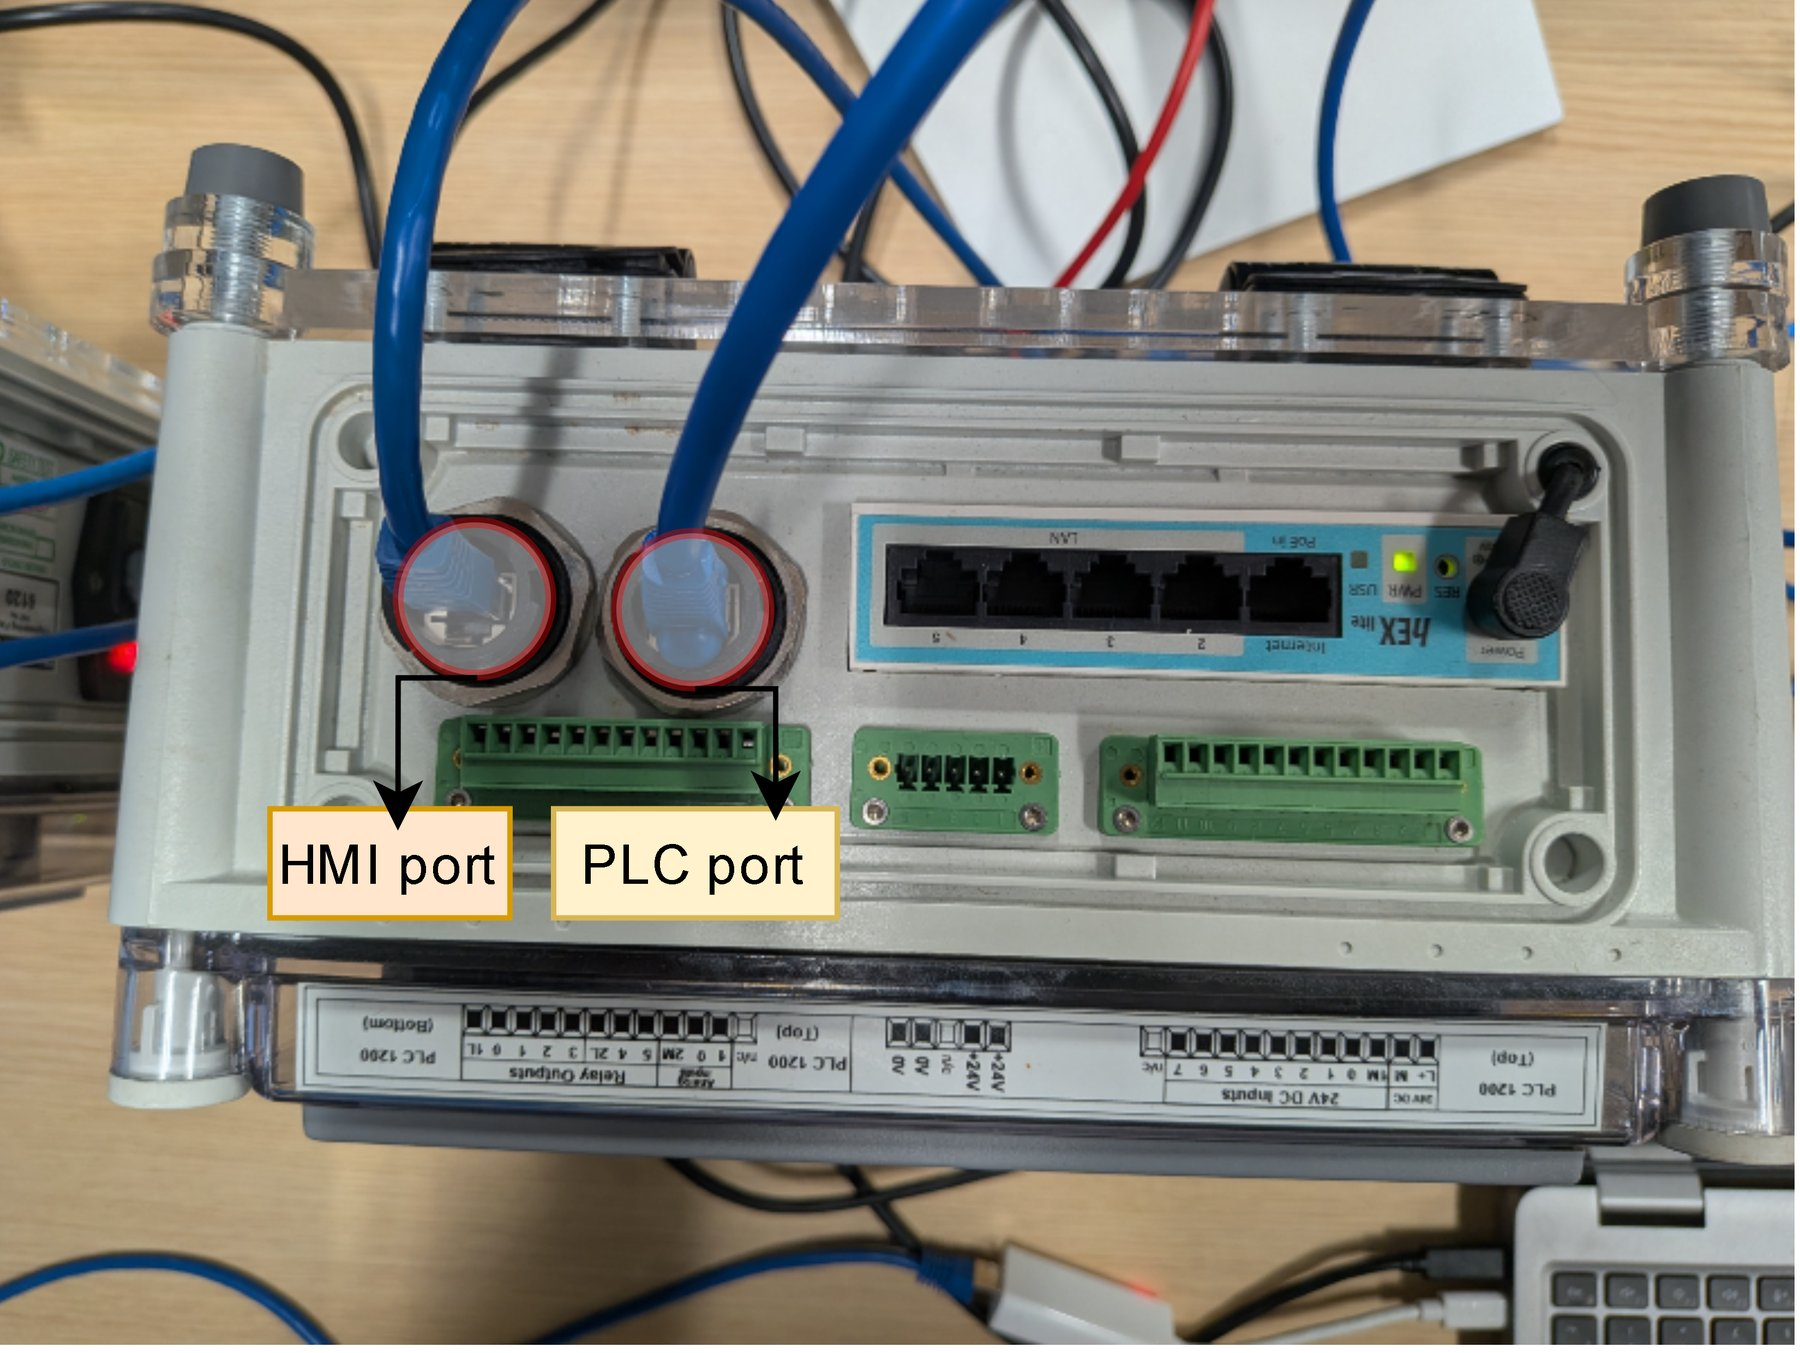
\includegraphics[width=0.82\textwidth]{photo_testbed_panel.jpg}
\caption{The physical process cell. The Siemens S7-1212C PLC and its operator HMI are wired into the cell through the labelled HMI and PLC network ports, which face the Open vSwitch fabric on Dell~1. The green terminal blocks carry the PLC's 24\,V digital inputs and relay outputs. Photographed on the testbed.}
\label{fig:hardware}
\end{figure}

\subsection{Nodes and devices}

Four machines make up the testbed. Dell~2 runs the CARS controller as an os-ken OpenFlow~1.3 application. Dell~1 runs the Open vSwitch fabric, the Snort sensor, and the supporting services, and hosts the simulated supervisory and attacker endpoints in Linux network namespaces. Dell~3 runs Cell-2. A Windows machine runs TIA Portal and Factory IO and acts as the engineering workstation. The two PLCs are Siemens S7-1200 units; PLC1 is a 1212C, model 6ES7~212-1BE40-0XB0 running firmware 4.2.3, confirmed by scanning it during evaluation. An operator HMI is present on each cell. The supervisory hosts, the SCADA or Modbus operator, the historian, the remediation agent and the Modbus unit, are realised as namespaces on Dell~1, each bound to a switch port, and the external attacker is a Kali Linux virtual machine on Dell~1 that is attached to the OT segment and holds no registered role.

\subsection{The two cells}

The fabric is divided into two process cells and a gateway, each an OpenFlow switch under the one controller. Cell-1, on switch \texttt{ovs1}, holds PLC1, which controls the critical tank, and its operator HMI. Cell-2, on switch \texttt{ovs2} on Dell~3, holds PLC2 and its HMI, reached through a network-address translation that presents their internal addresses \texttt{192.168.2.10} and \texttt{192.168.2.9} as \texttt{192.168.3.10} and \texttt{192.168.3.9} to the rest of the fabric; the translation lets the second cell reuse the Cell-1 addressing plan while remaining separately reachable. The gateway switch, \texttt{ovsgw}, carries the supervisory seams, the engineering and Factory IO host, the Snort mirror, the honeypot decoy, and the attacker vantage. The two cells and the gateway are joined by a patch link and a translated transit, so that all traffic to a protected asset crosses the CARS fabric and is subject to its policy. The fabric read directly from the switches with \texttt{ovs-vsctl show} is given in Figure~\ref{fig:ovsshow}: each bridge holds its OpenFlow connection to the controller, runs in secure fail mode, and presents the PLC and HMI on separate ports.

\begin{figure}[t]
\centering
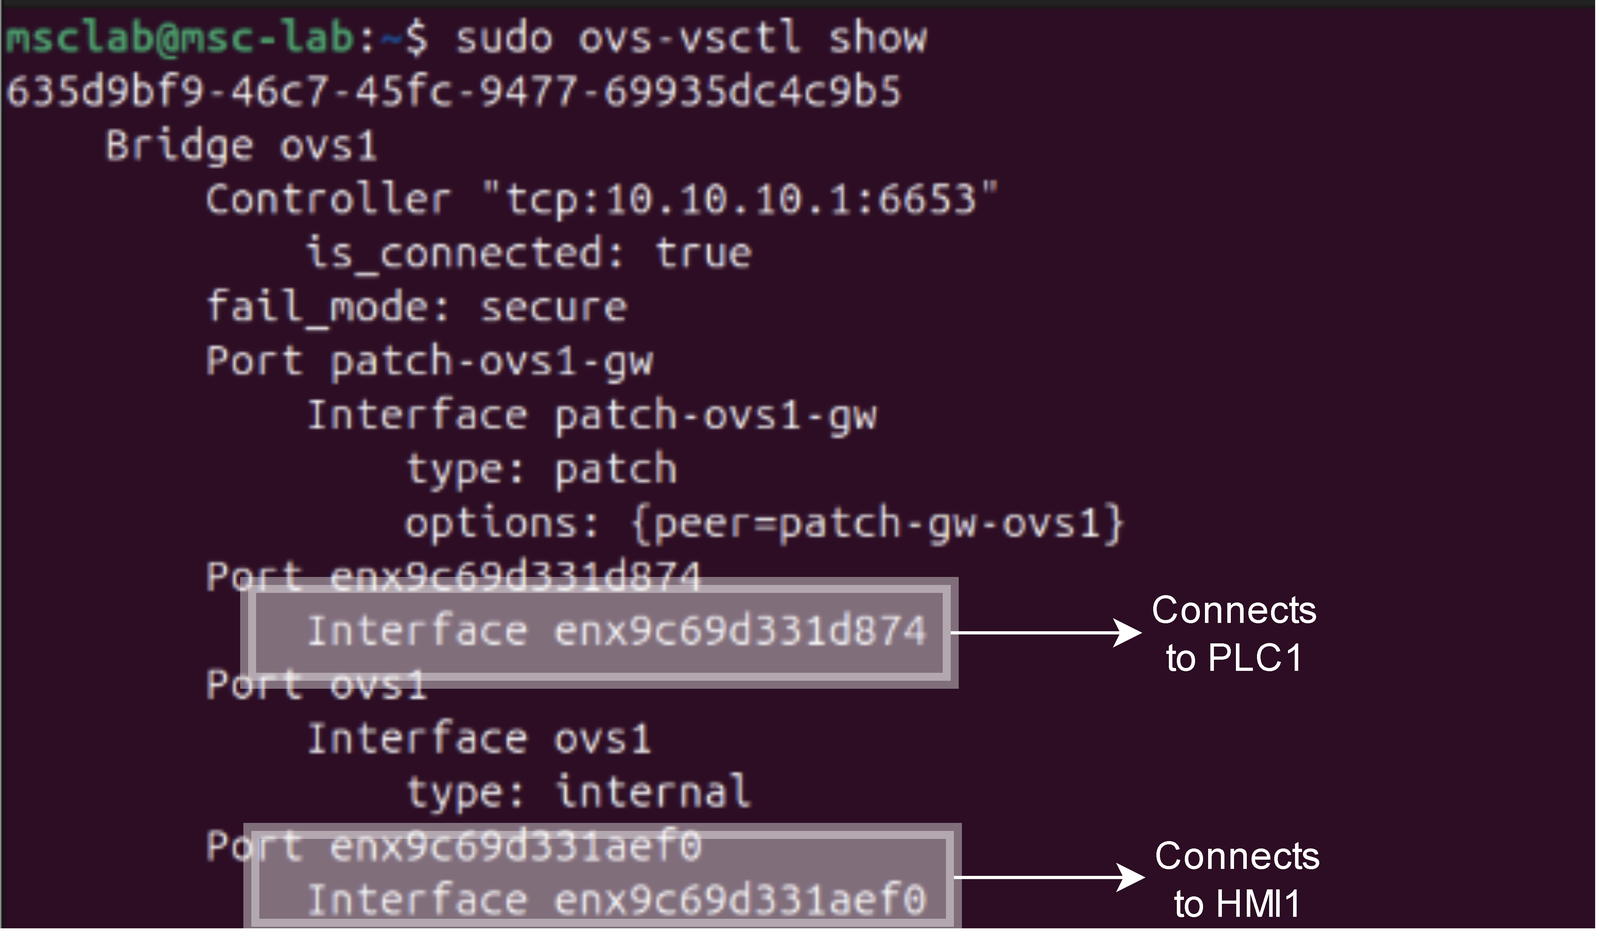
\includegraphics[width=0.86\textwidth]{term_ovs1_show.png}\\[6pt]
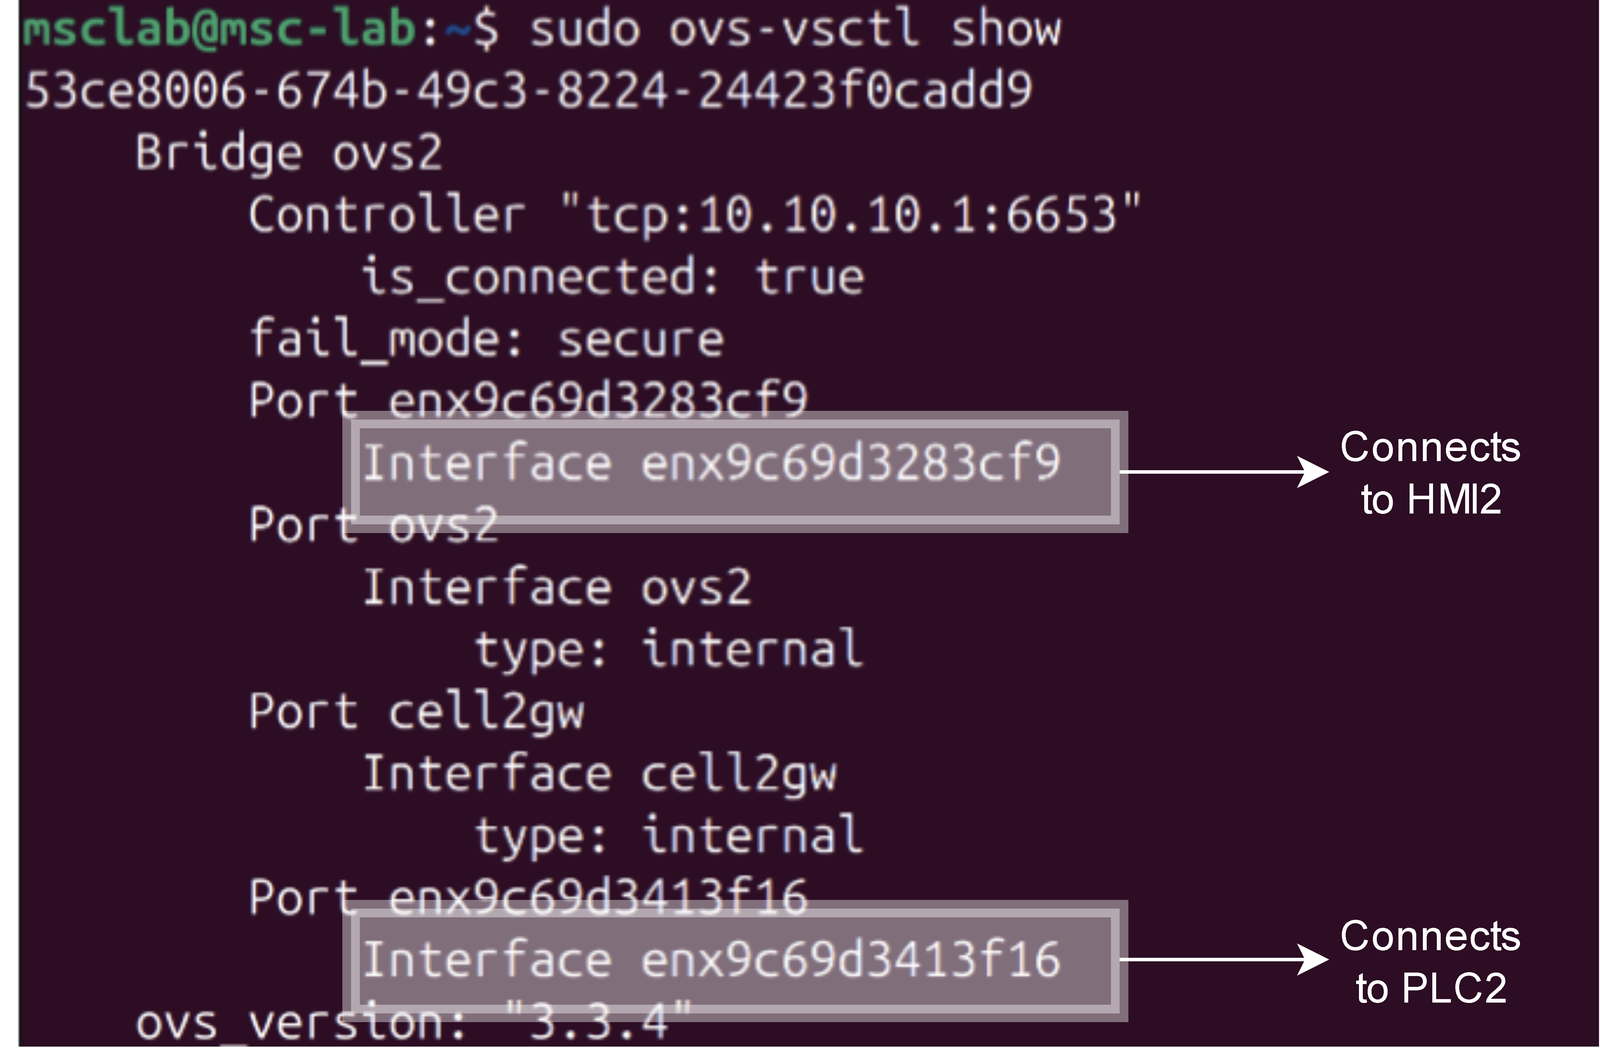
\includegraphics[width=0.86\textwidth]{term_ovs2_show.png}
\caption{The fabric read from the switches with \texttt{ovs-vsctl show}: Cell-1 (\texttt{ovs1}, top) and Cell-2 (\texttt{ovs2}, bottom). Each bridge is connected to the controller at \texttt{tcp:10.10.10.1:6653} with \texttt{fail\_mode: secure}, and carries its PLC and HMI on separate ports; \texttt{ovs1} also holds the patch to the gateway and \texttt{ovs2} the internal \texttt{cell2gw}. Captured live on 3 August 2026 (OVS 3.3.4); the arrows are annotations.}
\label{fig:ovsshow}
\end{figure}

\subsection{The physical process}

Cell-1 runs a live tank-level process, provided by Factory IO on the Windows machine and controlled by PLC1 over S7 across the fabric, as shown in Figure~\ref{fig:hil}. Factory IO supplies the level from a sensor and the state of the Start, Reset and Stop buttons as PLC inputs, and renders the fill valve, the discharge valve and the indicator lamps from the PLC outputs. The control runs in a cyclic block, OB30, which scales the raw sensor to a level of zero to one hundred, latches a running state from the operator buttons, and holds the level in a band by opening the fill valve below thirty and closing it above seventy against a constant discharge. The level that the PLC computes, held in a data block, is the process value that CARS protects; driving it out of its band, or blinding the PLC to it, is the physical harm the evaluation measures. The running scene and the operator HMI are shown in Figure~\ref{fig:process}, and the Factory IO driver that binds the scene to PLC1 in Figure~\ref{fig:driver}.

\begin{figure}[t]
\centering
\includegraphics[width=\textwidth]{{fig08_hil.drawio}.png}
\caption{The hardware-in-the-loop. Factory IO supplies the level and button inputs and renders the valve and lamp outputs; PLC1 runs the control in OB30; every exchange crosses the CARS fabric. Addresses and mappings are from the deployed project.}
\label{fig:hil}
\end{figure}

\begin{figure}[t]
\centering
\begin{minipage}[c]{0.50\textwidth}\centering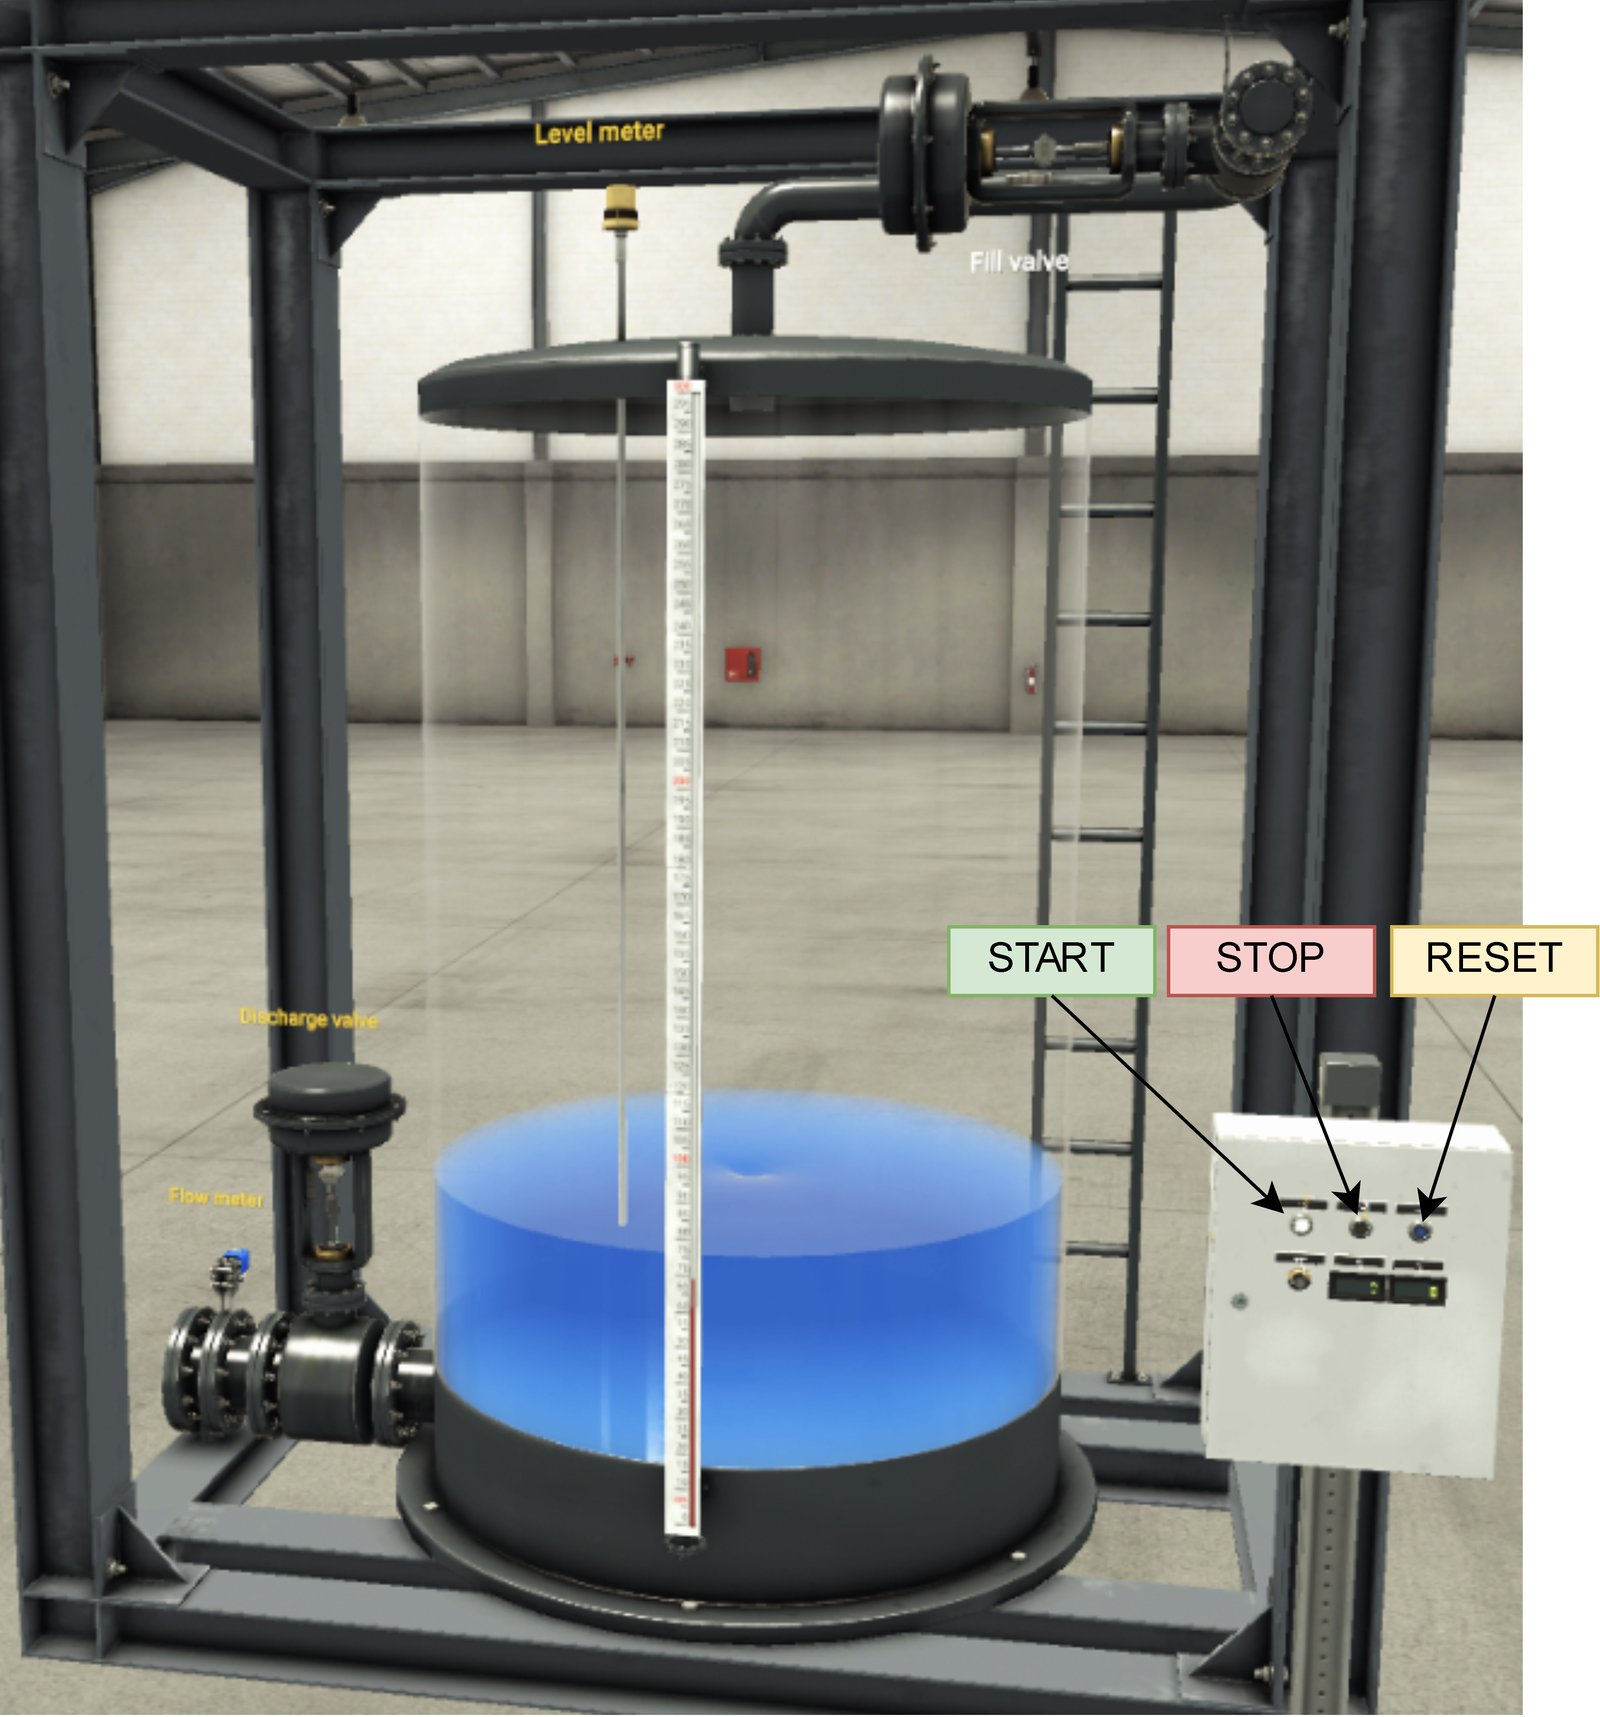
\includegraphics[width=\linewidth]{factoryio_scene.jpg}\end{minipage}\hfill
\begin{minipage}[c]{0.46\textwidth}\centering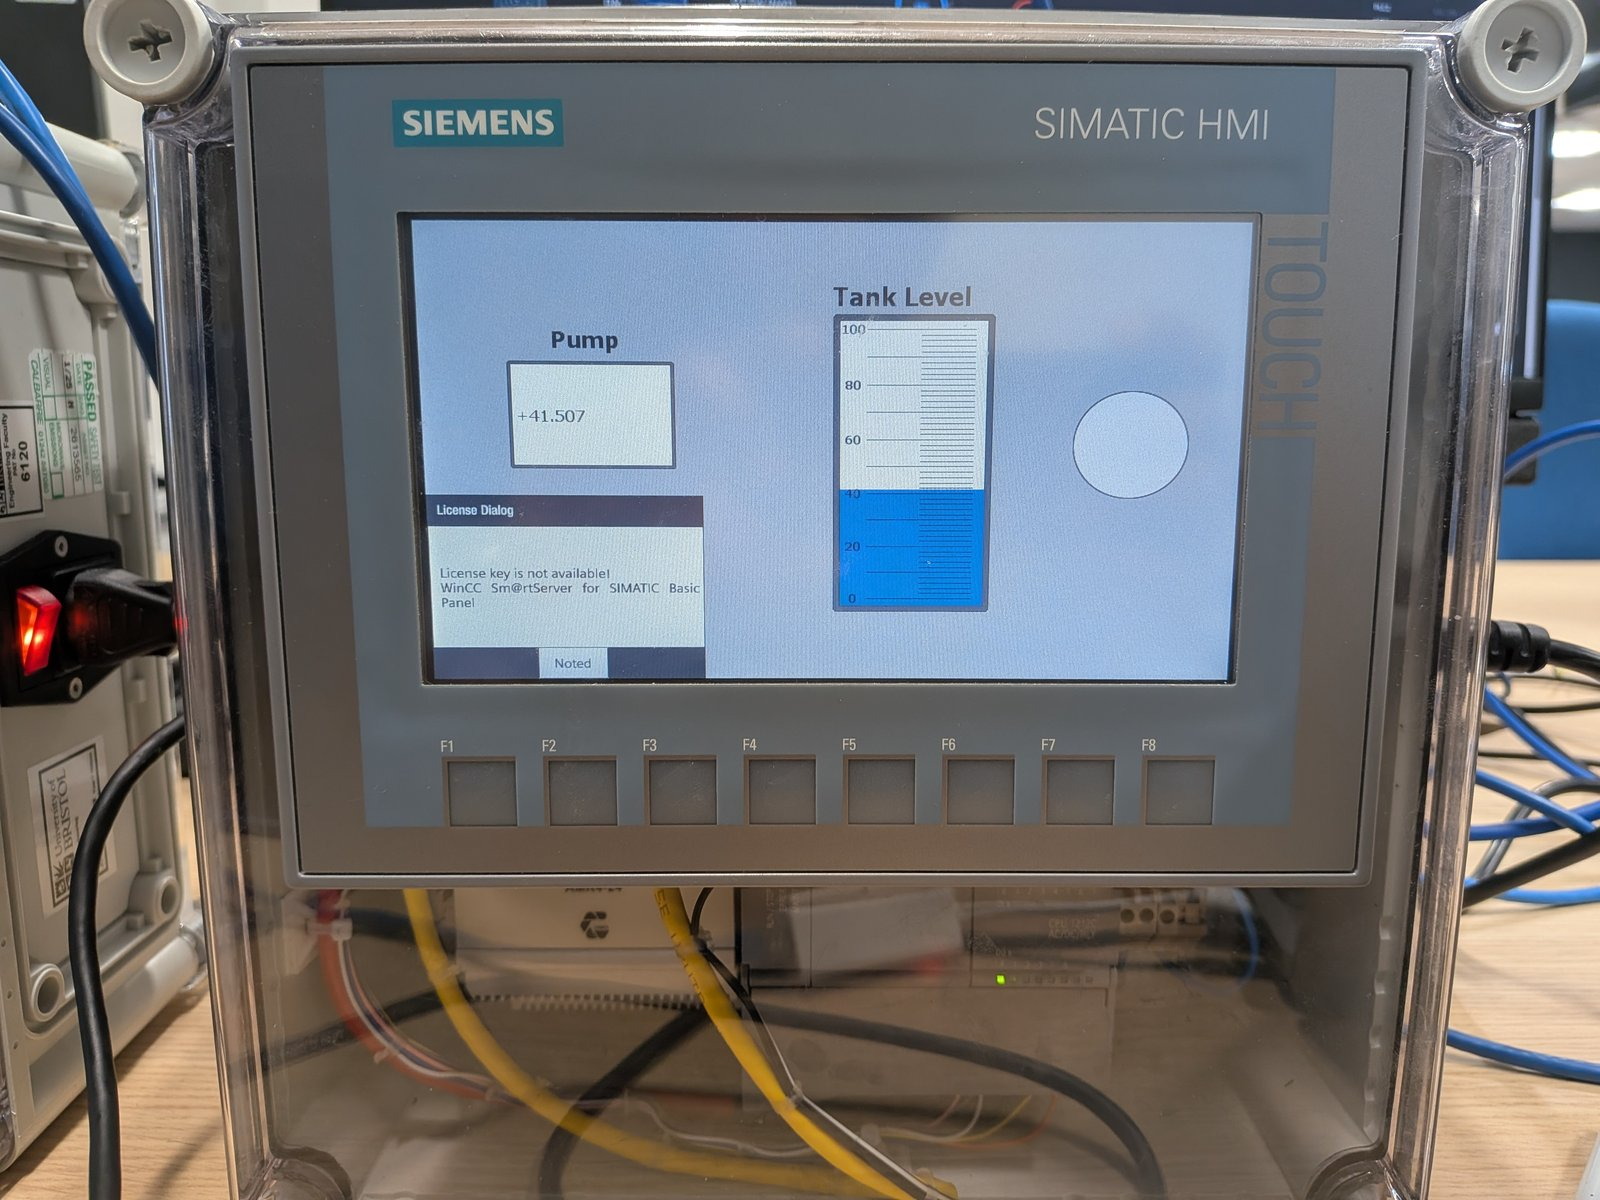
\includegraphics[width=\linewidth]{hmi1_tanklevel.jpg}\end{minipage}
\caption{The live process. Left: the Factory IO tank scene, with the level meter, the fill and discharge valves, the flow meter, and the Start, Stop and Reset station. Right: the operator HMI reading the tank level, here about 40 per cent, and the pump value. The scene runs on the Windows machine and exchanges its inputs and outputs with PLC1 over S7 across the fabric.}
\label{fig:process}
\end{figure}

\begin{figure}[t]
\centering
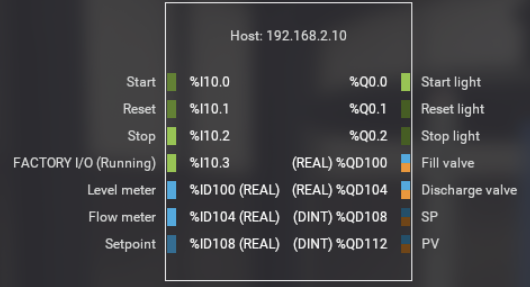
\includegraphics[width=0.58\textwidth]{factoryio_driver.png}
\caption{The Factory IO S7-1200 driver, bound to PLC1 at \texttt{192.168.2.10}. The inputs are the Start, Reset and Stop buttons at \texttt{\%I10.0}--\texttt{\%I10.2}, the running flag at \texttt{\%I10.3}, and the level, flow and setpoint values at \texttt{\%ID100}/\texttt{\%ID104}/\texttt{\%ID108}; the outputs are the lamps at \texttt{\%Q0.0}--\texttt{\%Q0.2}, the fill and discharge valves at \texttt{\%QD100}/\texttt{\%QD104}, and the setpoint and process value at \texttt{\%QD108}/\texttt{\%QD112}. Read from the deployed driver configuration; these match the OB30 tag table.}
\label{fig:driver}
\end{figure}

\section{CARS design overview}
\label{sec:designoverview}

CARS is placed as the enforcement point in the SDN fabric, between the operational hosts and the assets it protects, as shown in Figure~\ref{fig:overview}. Its design is layered. A proactive layer, always in force, binds each host's identity and admits only the connections on a short allowlist, so an unregistered host is refused before any operation is considered. A reactive layer recovers the operation from the traffic by deep packet inspection, decides its tier from the source role, the operation and the criticality of the target, and applies a graded response. A self-checking layer verifies the forwarding state against a trusted baseline and authenticates the control interface, so that a compromise of the control plane is caught rather than trusted.

\begin{figure}[t]
\centering
\includegraphics[width=0.85\textwidth]{{fig01_topology_highlevel.drawio}.png}
\caption{CARS in the fabric. All traffic to a protected asset crosses the SDN fabric, which the controller governs; the Factory IO process closes a hardware-in-the-loop with PLC1.}
\label{fig:overview}
\end{figure}

Two separations shape the design. The controller, which decides, is separate from the switches, which enforce, the standard software-defined split that lets one policy govern the whole fabric. The decision, which is a tier, is separate from the response, which is an action, so that a single judgement drives a graded ladder rather than one blunt action. Every response is bounded in time, reversible, and leaves an audit record, which is what allows an operator to enable it. The remaining sections detail each layer: the pipeline that enforces the policy (Section~\ref{sec:pipeline}), the criticality and operation model that decides (Section~\ref{sec:model}), and the reference implementation of the detection, the responses and the self-checks (Section~\ref{sec:implementation}).

\section{The enforcement pipeline}
\label{sec:pipeline}

CARS enforces its policy in the data plane as a pipeline of three OpenFlow tables, installed on every switch in the fabric so that the same rules apply in each cell. A packet reaches its destination only if it passes all three stages; failing any stage drops or diverts it. The pipeline is shown in Figure~\ref{fig:pipeline}. The flow rules quoted below are read from the running switches rather than from the source, and the full tables are reproduced in Appendix~\ref{appx:material}, so that the description matches the deployed system exactly.

\begin{figure}[t]
\centering
\includegraphics[width=0.9\textwidth]{{fig05_pipeline.drawio}.png}
\caption{The CARS OpenFlow pipeline, captured live on \texttt{ovs1} and \texttt{ovsgw}. A packet is admitted only if its identity binds at Table~0, its connection is permitted and tracked at Table~1, and it is then forwarded at Table~2. Proactive policy carries cookie \texttt{0x00a2}; reactive responses installed by the controller carry \texttt{0x00ca}.}
\label{fig:pipeline}
\end{figure}

Table~0 performs identity binding, the defence against spoofing. Each protected host is bound to the switch port, MAC address and IP address from which it is permitted to speak. A packet whose source matches its binding, at priority 200 for both IP and ARP, is passed to Table~1; traffic arriving on an inter-bridge link, which has already been checked at the far switch, is passed at priority 150. A packet that claims a protected address but arrives on any other port matches no binding and falls to a priority-100 rule that drops it, for both IP and ARP. Traffic that claims no protected address is passed on at priority 50. The effect is that an attacker cannot borrow the network identity of a trusted host: a forged source is dropped at ingress before it reaches the policy stage.

Table~1 is the stateful policy stage, and it carries connection state in the data plane in the manner introduced by AvantGuard \cite{shin2013avantguard}. An untracked packet is first submitted to connection tracking at priority 90 and re-enters the table. A packet belonging to an already established connection is admitted at priority 85, which is what allows a protected device such as the HMI to receive the replies to connections it began while remaining shielded from new inbound connections. New connections are then judged against the proactive policy. A small allowlist of conduits, each naming a source, a destination and a service port, is permitted and committed to the connection table at priority 80; the deployed policy holds nine such conduits, including the operator and engineering paths to PLC1 and the cross-cell collector path to PLC2. A new connection to a protected asset that matches no conduit is dropped at priority 55, the default-deny that closes an asset to everything except its named conduits, and a new connection to any other asset is committed and passed at priority 10. The reactive responses described in Section~\ref{sec:model} are installed into this same table by the controller at higher priorities, so that an isolate or a block takes precedence over the proactive rules for as long as an attack persists.

Table~2 forwards. It floods broadcast traffic, sends a packet whose source and destination MAC pair has been learned to the correct port, and refers an unknown destination to the controller so that the source can be learned. Separating the three concerns, identity at Table~0, connection state and policy at Table~1, and forwarding at Table~2, means each is enforced on its own, and a packet cannot reach forwarding by evading an earlier stage.

The proactive rules carry the cookie \texttt{0x00a2} and the reactive rules carry \texttt{0x00ca}. This separation is used by the flow-integrity checker of Section~\ref{sec:implementation} to tell the fixed policy from the responses installed at run time.

\section{The criticality and operation model}
\label{sec:model}

CARS makes two kinds of decision. At the connection level a proactive policy fixes which parties may open a connection to which asset at all. At the operation level each permitted exchange is judged by the role of its source, the operation it carries, and the criticality of the asset it targets. This section defines the model; the pipeline of Section~\ref{sec:pipeline} enforces it. Every value quoted is taken from the deployed controller.

\subsection{Asset criticality}

Every protected asset is assigned a criticality tier by the consequence of its compromise, following the consequence-based approach set out in Section~\ref{sec:criticality} \cite{inl2016cce, cisa2025assetinventory}. Table~\ref{tab:criticality} lists the tiers on the testbed. Each tier carries a weight from three down to zero, and the weight does two things in the response. It sets the duration of a block or an isolate, computed as thirty seconds plus fifteen for each unit of weight, so a critical asset holds an attacker out for seventy-five seconds against thirty for a low one, and it brings escalation forward, so a higher-consequence asset reaches a cut sooner. Criticality therefore shapes not only whether CARS acts but how hard and for how long.

\begin{table}[t]
\centering
\begin{tabular}{llccc}
\hline
Asset & Address & Role & Criticality & Weight \\
\hline
PLC1 & 192.168.2.10 & plc & CRITICAL & 3 \\
PLC2 & 192.168.3.10 & plc & HIGH & 2 \\
HMI1 & 192.168.2.9 & hmi & HIGH & 2 \\
HMI2 & 192.168.3.9 & hmi & MEDIUM & 1 \\
Historian & 192.168.2.30 & historian & MEDIUM & 1 \\
Modbus unit & 192.168.2.20 & plc & LOW & 0 \\
\hline
\end{tabular}
\caption{Asset criticality on the testbed, from the deployed controller (confirmed against the \texttt{/cars/criticality} interface, Figure~\ref{fig:criticality}). The weight scales the response: a block or isolate lasts $30 + 15w$ seconds, and escalation is faster at higher weight.}
\label{tab:criticality}
\end{table}

\begin{figure}[t]
\centering
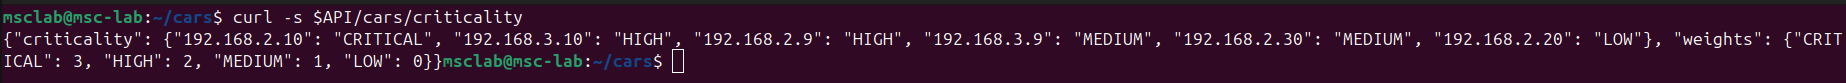
\includegraphics[width=\textwidth]{term_criticality.png}
\caption{The criticality read live from the controller with \texttt{curl \$API/cars/criticality}, backing Table~\ref{tab:criticality}: the six tiered assets and the weight of each tier. Captured on 3 August 2026.}
\label{fig:criticality}
\end{figure}

\subsection{Roles and operations}

Each host has a role in the registry: \emph{plc}, \emph{hmi}, \emph{historian}, \emph{scada}, \emph{ews} (engineering workstation), \emph{remediation}, or \emph{gateway}. A host with no registry entry, such as the external attacker, is \emph{unknown}. The operation carried by a packet is recovered from the industrial protocol by deep packet inspection (Section~\ref{sec:implementation}): a read of a value, a write of one, a control action on the process image, a diagnostic request, a program download, or a malformed request, together with the plain connection setup. Treating the operation as a first-class input is what lets CARS permit an engineer to read a PLC while refusing that same engineer a program download.

\subsection{The rulebook and criticality elevation}

The tier of an operation is decided by a rulebook of (source role, destination role, operation, tier) tuples, evaluated first match wins. Table~\ref{tab:rulebook} gives the rules; the full deployed ordering is reproduced in Appendix~\ref{appx:material}. The operator loop between HMI and PLC is tier CRITICAL and is never enforced against, a safety invariant so that the defence can never cut the loop that keeps the process safe. The dangerous operations are FORBIDDEN, subject to a deliberate ordering. A diagnostic, a program download or a malformed request is refused to a PLC or HMI from every source. A control write is refused from every source as well, except the two that are pre-authorised for it and whose rows are placed before the block, the engineering workstation and the remediation agent, so their legitimate actuation of the PLC classifies as OPERATIONAL rather than FORBIDDEN. Routine reads from the supervisory roles are OPERATIONAL, and an actuating write from a supervisory, historian or scada role is SENSITIVE. On top of the first match, one rule adjusts the tier by criticality: a SENSITIVE operation aimed at a CRITICAL asset, outside an authorised maintenance window, is elevated to FORBIDDEN, because nothing but the control loop and an authorised engineer may actuate the safety-critical process. The decision is shown in Figure~\ref{fig:decision}. The resulting tier and the observed rate then select a graded response, which is described in Section~\ref{sec:implementation}.

\begin{table}[t]
\centering
\begin{tabular}{lll l}
\hline
Source role & Destination & Operation & Tier \\
\hline
hmi, plc (the loop) & plc, hmi & any & CRITICAL \\
remediation & plc & any & OPERATIONAL \\
ews & plc & read, write, control & OPERATIONAL \\
any & plc, hmi & control, diag, program, illegal & FORBIDDEN \\
ews & hmi & any & SENSITIVE \\
historian, scada, supervisory & plc, hmi & write & SENSITIVE \\
historian, scada, supervisory & plc, hmi & any & OPERATIONAL \\
any & any & any & FORBIDDEN \\
\hline
\end{tabular}
\caption{The rulebook, evaluated first match wins (rows with a shared tier grouped for presentation; the exact deployed order is in Appendix~\ref{appx:material}). A SENSITIVE operation on a CRITICAL asset, outside a maintenance window, is elevated to FORBIDDEN.}
\label{tab:rulebook}
\end{table}

\begin{figure}[t]
\centering
\includegraphics[width=0.82\textwidth]{{fig04_decision.drawio}.png}
\caption{The CARS operation decision. The source role and operation give a tier by first match in the rulebook; a sensitive operation on a critical asset is elevated to forbidden; the tier and the observed rate then select the graded response.}
\label{fig:decision}
\end{figure}

\subsection{Proactive policy}

Alongside the per-operation decision, a proactive policy fixes which connections may exist at all, independently of any live detection. It is a short allowlist of conduits, each a source, a destination and a service port, together with a default-deny on the protected assets. The deployed policy, loaded from a run-time file and installed as the priority-80 and priority-55 flows of Section~\ref{sec:pipeline}, holds nine conduits: the operator, engineering, remediation and historian paths to PLC1; the operator and historian paths to the Modbus unit; the engineering path to HMI1; and the Cell-2 collector path to PLC2. Every other new connection to PLC1, HMI1 or the Modbus unit is denied. An unregistered host is therefore refused at the connection level before any operation is considered, while the rulebook governs what the permitted parties may then do.

\section{Reference implementation}
\label{sec:implementation}

The design of the preceding sections is realised on the testbed as an os-ken OpenFlow~1.3 controller on Dell~2, an Open vSwitch fabric and a Snort sensor on Dell~1, and the pipeline of Section~\ref{sec:pipeline}. This section describes how each mechanism is built. The values quoted are read from the running system.

\subsection{Identity binding and connection state}

Table~0 realises the anti-spoof binding as OpenFlow rules. Each protected host has a rule, at priority 200, that matches its ingress port, source MAC and source address, for both IP and ARP, and passes the packet on; a companion priority-100 rule drops any packet that claims the same address from any other port. The bindings are pinned to fixed ofports, so that re-cabling cannot silently move a host and break its binding, a fault observed and corrected during development. Table~1 carries connection state using the switch's connection-tracking action: an untracked packet is submitted to conntrack and re-enters the table, an established connection is admitted, and only a handshaked new connection that matches a conduit is committed. Because state is held in the data plane rather than at the controller, an out-of-state packet that a stateless rule would pass is refused without a round trip to the control plane, in the manner of AvantGuard \cite{shin2013avantguard}. The full flow tables dumped from all three switches are reproduced in Appendix~\ref{appx:flows}, the deployed decision logic in Appendix~\ref{appx:logic}, the Snort detection rules in Appendix~\ref{appx:snort}, and a snapshot of the live runtime state in Appendix~\ref{appx:runtime}.

\subsection{Operation classification}

The operation carried by a packet is recovered by deep packet inspection. A Snort sensor reads a mirror of the gateway switch and matches the function field of each industrial request. For S7comm to a PLC on port 102, the function byte that follows the protocol header distinguishes a read (\texttt{0x04}), a write or control action (\texttt{0x05}), and the diagnostic control and stop functions (\texttt{0x28} and \texttt{0x29}). For Modbus to the simulated unit on port 502, the function code distinguishes a register read (\texttt{0x03}), coil and register writes (\texttt{0x05}, \texttt{0x06}, \texttt{0x0F}, \texttt{0x10}), a diagnostic (\texttt{0x08}) and the encapsulated-interface program function (\texttt{0x2B}); any function code above the defined range is flagged as malformed. Figure~\ref{fig:ops} summarises the mapping. Each match raises an alert that names the operation, which is what allows the decision of Section~\ref{sec:model} to treat the same connection differently according to what it carries.

\begin{figure}[t]
\centering
\includegraphics[width=0.9\textwidth]{{fig07_ops.drawio}.png}
\caption{Operation classes recovered by deep packet inspection from the S7comm and Modbus function fields, as encoded in the deployed Snort rules.}
\label{fig:ops}
\end{figure}

\subsection{From detection to response}

Detection and response are joined by the chain shown in Figure~\ref{fig:detresp}. Snort writes each alert to a file; a bridge process follows the file and forwards each alert, with its source, destination and recovered operation, to the controller's \texttt{/cars/respond} interface; the controller classifies the operation against the rulebook and criticality, selects a response, and installs the corresponding flow rule. The controller's own decision time is 0.024\,ms on average over the run captured here, so the path from a packet on the wire to an installed rule completes in the low milliseconds.

\begin{figure}[t]
\centering
\includegraphics[width=0.95\textwidth]{{fig06_detresp.drawio}.png}
\caption{The detection-to-response path: a mirrored packet is classified by Snort, the alert is forwarded to the controller, which decides against the rulebook and criticality and installs the flow rule that enforces the response.}
\label{fig:detresp}
\end{figure}

\subsection{The response ladder}

The controller selects one of seven graded responses and realises it in OpenFlow. ALLOW and MONITOR admit the traffic and record it. THROTTLE attaches a rate-limiting meter to the conduit. DEFLECT rewrites the destination to a honeypot and installs the forward and reverse rules for it. ISOLATE drops all traffic from the offending source at priority 110, and BLOCK drops the single offending conduit at priority 100. REFUSE is reserved for the safety-critical loop and only mirrors and alerts, never enforcing, so that the operator's control of the process can never be cut by the defence. Every reactive rule carries the cookie \texttt{0x00ca} and a criticality-scaled timeout, so it expires and self-heals unless the attack persists.

\subsection{Forwarding integrity and control authentication}

Two mechanisms protect CARS against a compromised control plane, the threat identified by Gardiner et al.\ \cite{gardiner2021controller}. A flow-integrity checker holds a trusted baseline of the proactive policy, distinguished by its cookie \texttt{0x00a2}, and compares the live tables against it every ten seconds; a rule that is missing, added or altered, other than the reactive rules under cookie \texttt{0x00ca}, is reported as drift, catching bogus injected rules, black-holes and removals in the manner of the policy checker of Melis et al.\ \cite{melis2018policychecker}. Separately, every state-changing control operation, such as disarming the defence, requires an authentication token, so a host that reaches the control interface cannot silently switch CARS off; an unauthenticated attempt is refused and logged.

\section{Deployment}
\label{sec:deployment}

CARS is deployed across the four machines of the testbed as shown in Figure~\ref{fig:deployment}. The arrangement keeps the two planes apart: the controller, which decides, is separate from the switches, which enforce, and the sensing sits with the fabric so that detection stays close to the traffic while the decision stays central.

\begin{figure}[t]
\centering
\includegraphics[width=\textwidth]{{fig03_deployment.drawio}.png}
\caption{Deployment. The controller on Dell 2 governs the switches on Dell 1 and Dell 3 over the OpenFlow control plane; the fabric, the Snort sensor and the supporting agents run together on Dell 1, and the engineering workstation with Factory IO is the live process.}
\label{fig:deployment}
\end{figure}

The controller runs on Dell 2 as an os-ken application, \texttt{cars\_engine.py}, launched with link observation enabled. It holds the whole decision logic described in Section~\ref{sec:model}, speaks OpenFlow~1.3 to the switches on port \texttt{6653}, and exposes the control interface used for responses and for the guarded operations on port \texttt{8080}. Nothing else of CARS runs on this node. It runs continuously and prints each decision as it is taken; a live extract is shown in Figure~\ref{fig:decisionlog}, and its status interface (Figure~\ref{fig:status}) reports the three switches connected and both guards enabled.

\begin{figure}[t]
\centering
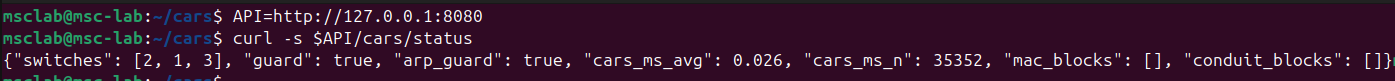
\includegraphics[width=\textwidth]{term_status.png}
\caption{The controller status from \texttt{curl \$API/cars/status}: the three switches connected (datapath identifiers \texttt{2}, \texttt{1}, \texttt{3}), identity and ARP guards enabled, and the running mean decide time. Captured on 3 August 2026.}
\label{fig:status}
\end{figure}

\begin{figure}[t]
\centering
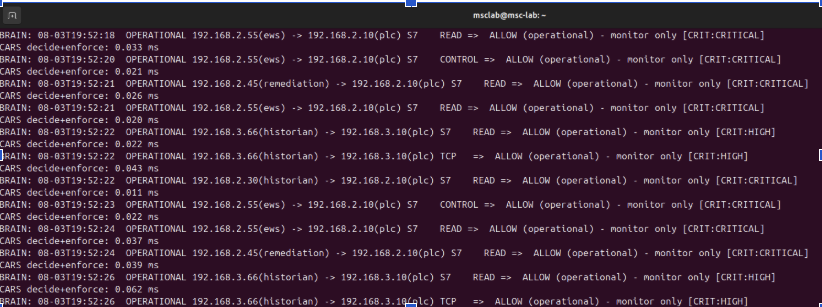
\includegraphics[width=0.95\textwidth]{term_decision_log.png}
\caption{The deployed controller running live on Dell~2. Each line records one decision: the source and destination, the protocol and operation, the verdict and response, the asset criticality, and the decide-and-enforce time. Captured from the controller console on 3 August 2026, confirming the engine runs as a service and logs every decision.}
\label{fig:decisionlog}
\end{figure}

The fabric and the sensing run on Dell 1. The two Open vSwitch bridges, \texttt{ovs1} for Cell-1 and \texttt{ovsgw} for the gateway, carry the data plane. The Snort sensor reads a mirror of the gateway traffic and hands its findings to a small bridge, \texttt{cars-bridge}, which posts them to the controller at \texttt{/cars/respond}; this is the detection path of Section~\ref{sec:implementation}. Three supporting services run alongside: the flow-integrity checker, \texttt{cars-flowaudit}, which polls the tables every ten seconds against the trusted baseline; the remediation agent on \texttt{192.168.2.45}; and the decision dashboard. The operator, attacker and service endpoints are hosted in Linux network namespaces on this node, which is why a single machine can present the operator station, the Modbus device, the honeypot and the attacker vantage on distinct addresses.

Cell-2 runs on Dell 3 with its own switch, \texttt{ovs2}, and the address-translation clone that lets it re-use the Cell-1 plan, as described in Section~\ref{sec:testbed}. The Windows machine runs TIA Portal and Factory IO; it is both the engineering workstation, at \texttt{192.168.2.55}, and the physical process of the hardware-in-the-loop. One boundary follows from this layout: the Snort mirror is on the gateway, so traffic that stays within Cell-2 on \texttt{ovs2} is enforced by the proactive policy but is not seen by the detector. The reactive layer therefore covers the paths that cross the gateway, which is where the supervisory and cross-cell conduits run.

\chapter{Critical Evaluation}
\label{chap:evaluation}

\section{Method and metrics}
\label{sec:evalmethod}

The first question for a reactive defence in an operational network is not whether it can block an attack but whether it can be trusted not to block legitimate work. A false positive that cuts a control conduit is the deployment barrier, so the evaluation measures decision accuracy across the whole space of source role, operation and target criticality on the testbed, and reports the false-positive rate as the headline figure.

Each case is a tuple of source, destination, operation and rate, carrying a ground-truth label assigned from security intent: legitimate, attack, grey (criticality-graded) or flood-exempt. The measured decision is the deployed engine's own verdict, obtained by posting the case to the controller's \texttt{/cars/respond} interface, which runs the exact production path: the first-match classification of (role, operation) to a tier, the criticality elevation of a SENSITIVE operation on a CRITICAL asset, and the graded response selection. The engine is not reimplemented for the test; the labelled set is driven through it. The pass runs with enforcement disarmed, so it measures pure decisions with no side effect on the live conduits, then re-arms.

The verdicts follow the intent. A legitimate case is a true negative if it is permitted, that is ALLOW, MONITOR, or REFUSE, the last being the safety loop that is mirrored and alerted but never cut, and a false positive if it is restricted. An attack case is a true positive if it is restricted, that is THROTTLE, DEFLECT, ISOLATE or BLOCK, and a false negative if it is permitted. Grey cases are shown to demonstrate grading rather than scored: they test how the response scales with criticality, not a binary legitimate-or-attack decision, so they carry no true or false label by construction. All three are nonetheless handled correctly, and including them would leave the accuracy unchanged. The matrix was regenerated on the live system for this writeup and reproduces the stored baseline row for row; the decisions are corroborated at the packet level by the campaign of Section~\ref{sec:evalcampaign}, so the verdicts are not decision-only artefacts.

\section{Decision accuracy and false positives}
\label{sec:evalaccuracy}

Table~\ref{tab:accuracy} gives the full case set as measured. Of the twenty-four scored cases every one is classified correctly: thirteen true positives, eleven true negatives, no false positives and no false negatives, a decision accuracy of 100\% and, the figure that matters for deployment, a false-positive rate of 0\%. The confusion summary is Table~\ref{tab:confusion}. The full case set, with the inputs and the verdict for each case, is reproduced in Appendix~\ref{appx:matrix}. The twenty-four is not an arbitrary sample but the closure of the decision space: one case per reachable branch of the classification, elevation and response-selection path, so that every rule the engine can apply is exercised at least once and none is duplicated. A twenty-fifth case on the same branches would add no coverage. This is exhaustive coverage of the policy as deployed on this testbed, not a claim that the same rulebook generalises unchanged to another plant's assets and operations: it establishes correctness of the decision logic here, not deployment-grade confidence for industrial traffic at large.

Coverage establishes correctness on every branch; a larger run establishes that it holds at scale. A corpus of 2{,}078 labelled cases was driven through the same decision-only path with the harness \texttt{vast\_accuracy.py}: fifty-one unregistered attacker sources against an asset of every tier, across read, write, control and diagnostic operations at normal and flood rates, giving 2{,}040 attack cases, together with the legitimate supervisory conduits at sub-flood rates and the flood-exempt high-rate input, which form the false-positive test. The engine classified all 2{,}078 correctly: 2{,}040 true positives, 38 true negatives, no false positives and no false negatives, a decision accuracy of 100\% with a 95\% Wilson confidence interval of $[0.9982, 1.0000]$. Not one of the 2{,}040 attack variants was permitted, and no legitimate or exempt case was cut. The false-negative result carries statistical weight on its own count of 2{,}040; the zero false-positive rate rests on these 38 legitimate and exempt cases together with the live campaign of Section~\ref{sec:evalcampaign}, because the legitimate input space is bounded by the allowlist rather than by the number of trials. Like the scored matrix, this remains a single-platform, single-policy validation on the same testbed: it strengthens confidence in the decision logic itself, but it is not evidence that the result transfers to a different fabric, asset mix or rulebook, and it should not be read as production-proven.

\begin{table}[t]
\centering
\footnotesize
\begin{tabular}{llllcl}
\hline
Src$\to$Dst & Operation & Tier & Response & V & Case \\
\hline
\multicolumn{6}{l}{\textit{Legitimate benign (false-positive test)}} \\
9$\to$10 & READ & CRITICAL & REFUSE & TN & HMI$\to$PLC1 read (loop) \\
9$\to$10 & WRITE & CRITICAL & REFUSE & TN & HMI$\to$PLC1 setpoint (loop) \\
10$\to$9 & READ & CRITICAL & REFUSE & TN & PLC1$\to$HMI reply (loop) \\
55$\to$10 & READ & OPERATIONAL & ALLOW & TN & EWS/Factory IO read (HIL) \\
55$\to$10 & CONTROL & OPERATIONAL & ALLOW & TN & EWS/Factory IO write (HIL) \\
45$\to$10 & CONTROL & OPERATIONAL & ALLOW & TN & Remediation restore \\
30$\to$10 & READ & OPERATIONAL & ALLOW & TN & Historian poll PLC1 \\
30$\to$20 & READ & OPERATIONAL & ALLOW & TN & Historian poll Modbus \\
31$\to$20 & READ & OPERATIONAL & ALLOW & TN & SCADA Modbus poll \\
31$\to$10 & READ & OPERATIONAL & ALLOW & TN & SCADA read PLC1 \\
\multicolumn{6}{l}{\textit{Grey, criticality-graded (shown, not scored)}} \\
31$\to$10 & WRITE & FORBIDDEN & ISOLATE & grey & SCADA write CRITICAL (elevated) \\
31$\to$20 & WRITE & SENSITIVE & THROTTLE & grey & SCADA write LOW Modbus \\
30$\to$9 & WRITE & SENSITIVE & THROTTLE & grey & Historian write HIGH HMI1 \\
\multicolumn{6}{l}{\textit{Attacks (true-positive / false-negative test)}} \\
77$\to$10 & TCP & FORBIDDEN & ISOLATE & TP & Kali outsider TCP \\
77$\to$10 & READ & FORBIDDEN & ISOLATE & TP & Kali outsider read \\
66$\to$20 & WRITE & FORBIDDEN & BLOCK & TP & Unknown write Modbus \\
31$\to$10 & CONTROL & FORBIDDEN & ISOLATE & TP & Compromised SCADA actuates \\
31$\to$10 & PROGRAM & FORBIDDEN & ISOLATE & TP & SCADA program download \\
55$\to$10 & PROGRAM & FORBIDDEN & ISOLATE & TP & EWS program download (no window) \\
55$\to$10 & DIAG & FORBIDDEN & ISOLATE & TP & EWS diagnostics \\
55$\to$10 & ILLEGAL & FORBIDDEN & ISOLATE & TP & Malformed S7 \\
1$\to$10 & READ & FORBIDDEN & ISOLATE & TP & Gateway reaches PLC (no conduit) \\
30$\to$10 & CONTROL & FORBIDDEN & ISOLATE & TP & Historian issues CONTROL \\
66$\to$10 & READ & FORBIDDEN & ISOLATE & TP & Unknown read PLC1 \\
\multicolumn{6}{l}{\textit{Flood (volumetric overlay)}} \\
30$\to$10 & READ (50) & OPERATIONAL & BLOCK & TP & Historian read flood \\
55$\to$10 & CONTROL (50) & OPERATIONAL & ALLOW & TN & EWS high-rate (flood-exempt) \\
31$\to$20 & READ (50) & OPERATIONAL & THROTTLE & TP & SCADA read flood on Modbus \\
\hline
\end{tabular}
\caption{The decision matrix, measured live from the deployed engine via \texttt{/cars/respond}. Hosts are \texttt{192.168.2.x} (last octet shown). Twenty-four scored cases: 13 TP, 11 TN, 0 FP, 0 FN; three grey cases show grading. Regenerated for this writeup; identical to the 3 August baseline. Full per-decision controller log in Appendix~\ref{appx:logs}.}
\label{tab:accuracy}
\end{table}

\begin{table}[t]
\centering
\begin{tabular}{lcc}
\hline
 & Permitted & Restricted \\
\hline
Actually legitimate (11) & 11 (TN) & 0 (FP) \\
Actually attack (13) & 0 (FN) & 13 (TP) \\
\hline
\end{tabular}
\caption{Confusion summary. Accuracy $24/24 = 100\%$; false-positive rate $0/11 = 0\%$; false-negative rate $0/13 = 0\%$.}
\label{tab:confusion}
\end{table}

Every legitimate operation is permitted, including the two that most tempt a blunt filter. The high-rate control stream from the engineering and Factory IO host is flood-exempt and passes at fifty writes per second, because that host drives the hardware-in-the-loop and its rate is expected. The operator loop between HMI and PLC is tier CRITICAL and carries the REFUSE marker, so it is watched but never enforced against. The 0\% false-positive rate on this traffic is the operator-trust result: the defence can be armed on the live process without cutting the work that keeps it running.

The three grey cases show the criticality grading on one operation class. A SCADA write to the CRITICAL PLC1 is elevated from SENSITIVE to FORBIDDEN and quarantined; the same role's write to the LOW Modbus unit stays SENSITIVE and is throttled; a historian write to the HIGH operator panel is throttled. The response scales with the target's criticality, not the operation alone.

The set also isolates the operation-awareness a five-tuple filter cannot reach. The identical conduit from SCADA to the Modbus unit draws three different verdicts by operation and rate alone: a read is allowed, a write is throttled as a SENSITIVE actuation, and a read driven to fifty per second is throttled as a volumetric abuse. The decision is made on the industrial operation, not the addresses and ports.

The matrix is exhaustive over the meaningful decision space of the testbed rather than a random sample: it covers every role, operation and criticality combination that arises here. The same verdicts are then corroborated on live traffic by the campaign of Section~\ref{sec:evalcampaign}, where the deployed engine judged every phase and logged on the order of a thousand decisions per run, and the legitimate loop and telemetry were permitted throughout with no false positive observed (Appendix~\ref{appx:logs}). The 100\% figure is therefore a statement about this system's decision logic, established over the decision space and confirmed on live traffic, not a statistical guarantee for an arbitrary production network; that scope is stated in Section~\ref{sec:threats}.

To probe further, the engine was driven across its entire decision domain, every source, asset, operation and rate combination on the testbed, 868 cases in all. It returned a defined verdict for each, and on inspection every verdict is consistent with the deployed policy: the unregistered attacker is isolated on every operation against every asset, high-rate operations are restricted as floods, non-allowlisted conduits are default-denied, and the supervisory roles keep their reads. Building an independent oracle for a policy this nuanced is itself error-prone, so this exhaustive pass is a totality and consistency check rather than a second accuracy figure. The one behaviour it highlights is that the trusted remediation agent may issue even dangerous operations to the PLC unblocked, the trusted-role exposure of Section~\ref{sec:threats}.

\section{Criticality-graded response}
\label{sec:evalcriticality}

The criticality model earns its place only if the target's importance changes the outcome. The sweep, rerun with \texttt{cars\_criticality\_proof.sh}, holds the actor and the operation fixed and varies only the target's tier, in three parts: the bounded elevation of the decision, the proportionality of the response, and the invariants that criticality must never break.

Elevation is bounded. A SENSITIVE operation on a CRITICAL asset is raised to FORBIDDEN, as the grey cases of Table~\ref{tab:accuracy} show for a SCADA write to PLC1, whereas a read is never elevated: the same SCADA reading the same CRITICAL PLC1 stays OPERATIONAL and is allowed. The model suspends this elevation within an authorised maintenance window (Section~\ref{sec:model}), so scheduled engineering is not blocked by the rule that protects the asset at other times.

Proportionality is measured on the response side. The same forbidden control, from the same harmless attacker, draws a reactive rule whose length scales with the target's weight: 75 seconds on the CRITICAL PLC1, 60 seconds on the HIGH PLC2, 45 seconds on the MEDIUM historian and 30 seconds on the LOW Modbus unit, each self-healing when it expires (Figure~\ref{fig:critsweep}). The duration follows $30 + 15w$ seconds for tier weight $w$, measured at all four tiers. The scaled quantity is the timeout; it is applied to whichever reactive rule the escalation state selects, a source ISOLATE once an attacker persists, or a single-conduit BLOCK on a first offence, as the MEDIUM case shows.

\begin{figure}[t]
\centering
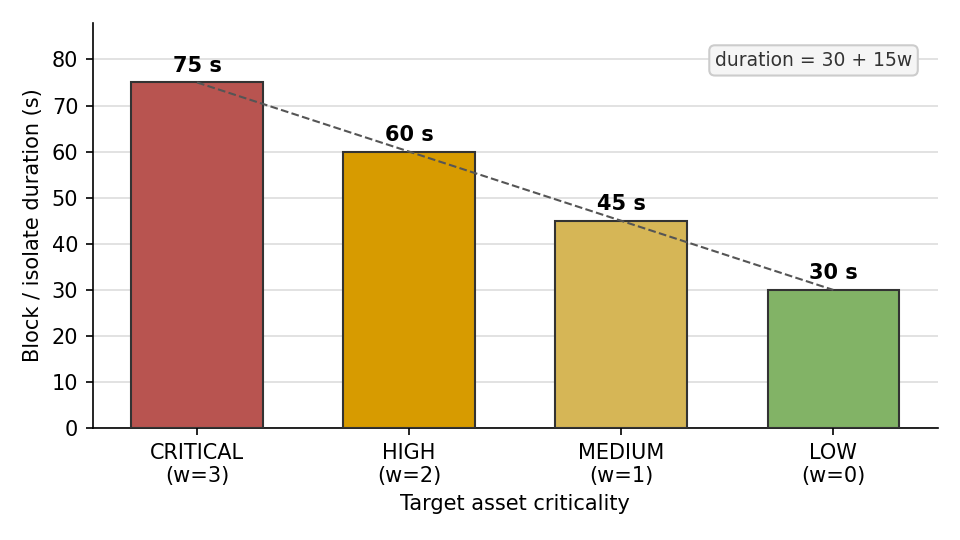
\includegraphics[width=0.78\textwidth]{chart_critsweep.png}
\caption{The reactive rule duration measured live for an identical forbidden control against targets of each criticality tier: 75, 60, 45 and 30 seconds for weights 3, 2, 1 and 0, following $30 + 15w$. Same actor and operation throughout; only the target's tier changes.}
\label{fig:critsweep}
\end{figure}

A larger run confirms the grading holds across operations and in combination, not one case at a time. Two hundred and forty decisions were driven through the deployed engine: an unregistered attacker and a compromised but trusted supervisory host, against all four tiers, across read, write, control and diagnostic operations, at normal and flood rates, and in both alternating and simultaneous bursts. The timeout tracks the target's tier throughout, 75, 60, 45 and 30 seconds, and the engine returned a correct verdict for every tier even when all four were attacked at once. The source is judged by what it does rather than by a blanket rule: the unregistered attacker is isolated on every operation, whereas the trusted host keeps its reads and is cut only on the operations its role must not perform. A flood withdraws the leniency a normal rate earns, so a permitted read on the critical asset is escalated from allowed to cut, and a source that keeps offending is treated more harshly as its offence count rises. The grading is stable across the full range of operation, rate, source and concurrency, not only the single-operation sweep of Figure~\ref{fig:critsweep}.

The invariants hold throughout. The operator control loop is never enforced against, even on the CRITICAL PLC1, where an HMI-to-PLC control returns REFUSE and is only mirrored and alerted, the safety cap of the model. Trusted monitoring is always allowed, even on the CRITICAL asset, where a SCADA read returns OPERATIONAL and passes. Criticality raises the response to a threat but never overrides the two rules that keep the process controllable.

\section{Wire-level campaign: armed versus unprotected}
\label{sec:evalcampaign}

The decision accuracy of Section~\ref{sec:evalaccuracy} is necessary but not sufficient; a decision matters only when it is enforced on the wire against a real attacker. This campaign exercises the defence at the packet level, comparing the armed system against the unprotected process. Unprotected has two honest meanings, kept separate: \emph{disarmed}, where reactive enforcement is switched off but CARS still detects and decides and the proactive structure stands, used for the insider and process vectors; and a true \emph{bypass} around the governed pipeline, used for the outsider vectors, since the proactive default-deny is always in force and merely disarming does not expose an unregistered host. Each vector is captured at three wire points, the PLC S7 port, the OpenFlow control channel and the Snort mirror. The legitimate Factory IO loop and the historian telemetry ran throughout and were permitted in every state, so the campaign carried zero false positives from end to end. Figure~\ref{fig:flow} shows what this means for a single attack packet in each state.

\begin{figure}[t]
\centering
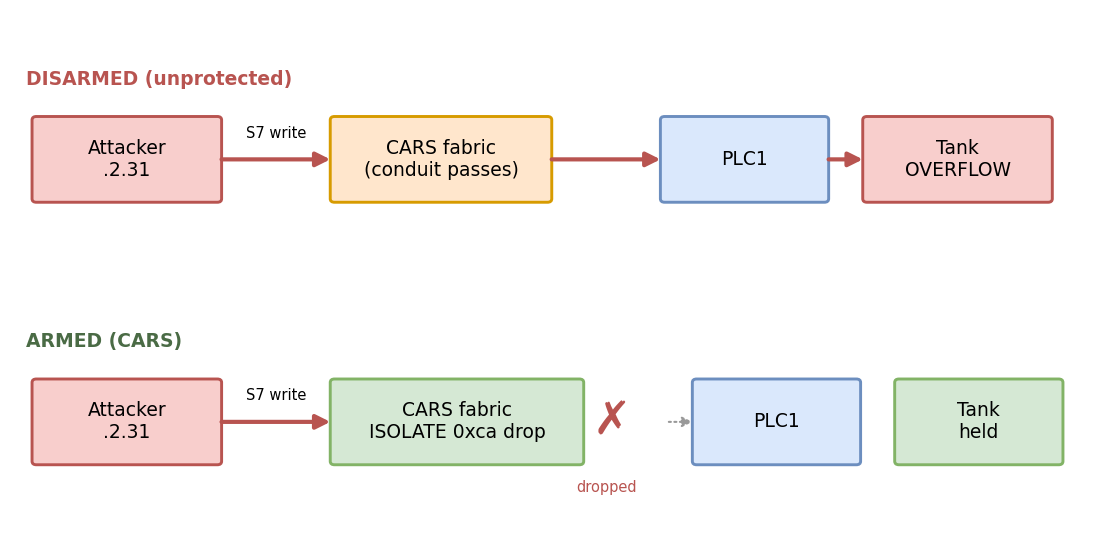
\includegraphics[width=0.92\textwidth]{flow_armed_vs_disarmed.png}
\caption{The path of a malicious S7 write in each state. Disarmed, the write crosses the fabric, reaches PLC1 and drives the tank to overflow. Armed, the reactive rule (\texttt{cookie 0x00ca}) drops it in the fabric, so it never reaches the PLC and the process is held.}
\label{fig:flow}
\end{figure}

\subsection{Process devastation and the deception}
\label{sec:evaldevastation}

The centrepiece is a false-data injection on the live tank, the attack that most directly threatens a physical process. A compromised supervisory host, \texttt{192.168.2.31}, writes the level sensor and the discharge valve in the process image over S7 at high rate, driving the tank past its safe band. Each write is a CONTROL operation to the CRITICAL PLC1. The disarmed and armed cases are compared on the same attacker, the same operation and the same target.

Disarmed, the injection runs unimpeded and the process is devastated. The tank is driven clean over the top: the Factory IO vessel fills completely and the operator panel's high-level alarm fires, the level cresting past the full mark at about 104\% (Figure~\ref{fig:p6overflow}). A sensor-spoof variant of the same attack instead pins the reported level near zero, so the operator sees a safe, empty tank while the real one fills, the deception at the heart of a process attack (Appendix~\ref{appx:scenarios}). Either way, while the attacker holds the actuators the operator cannot regain control.

\begin{figure}[t]
\centering
\begin{minipage}[c]{0.38\textwidth}\centering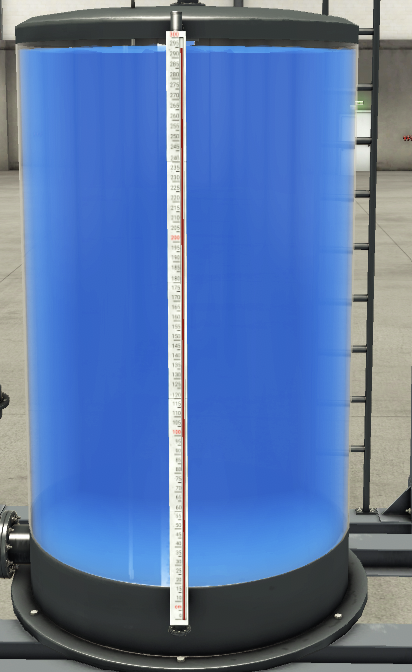
\includegraphics[width=\linewidth]{p6_overflow_tank.png}\end{minipage}\hfill
\begin{minipage}[c]{0.60\textwidth}\centering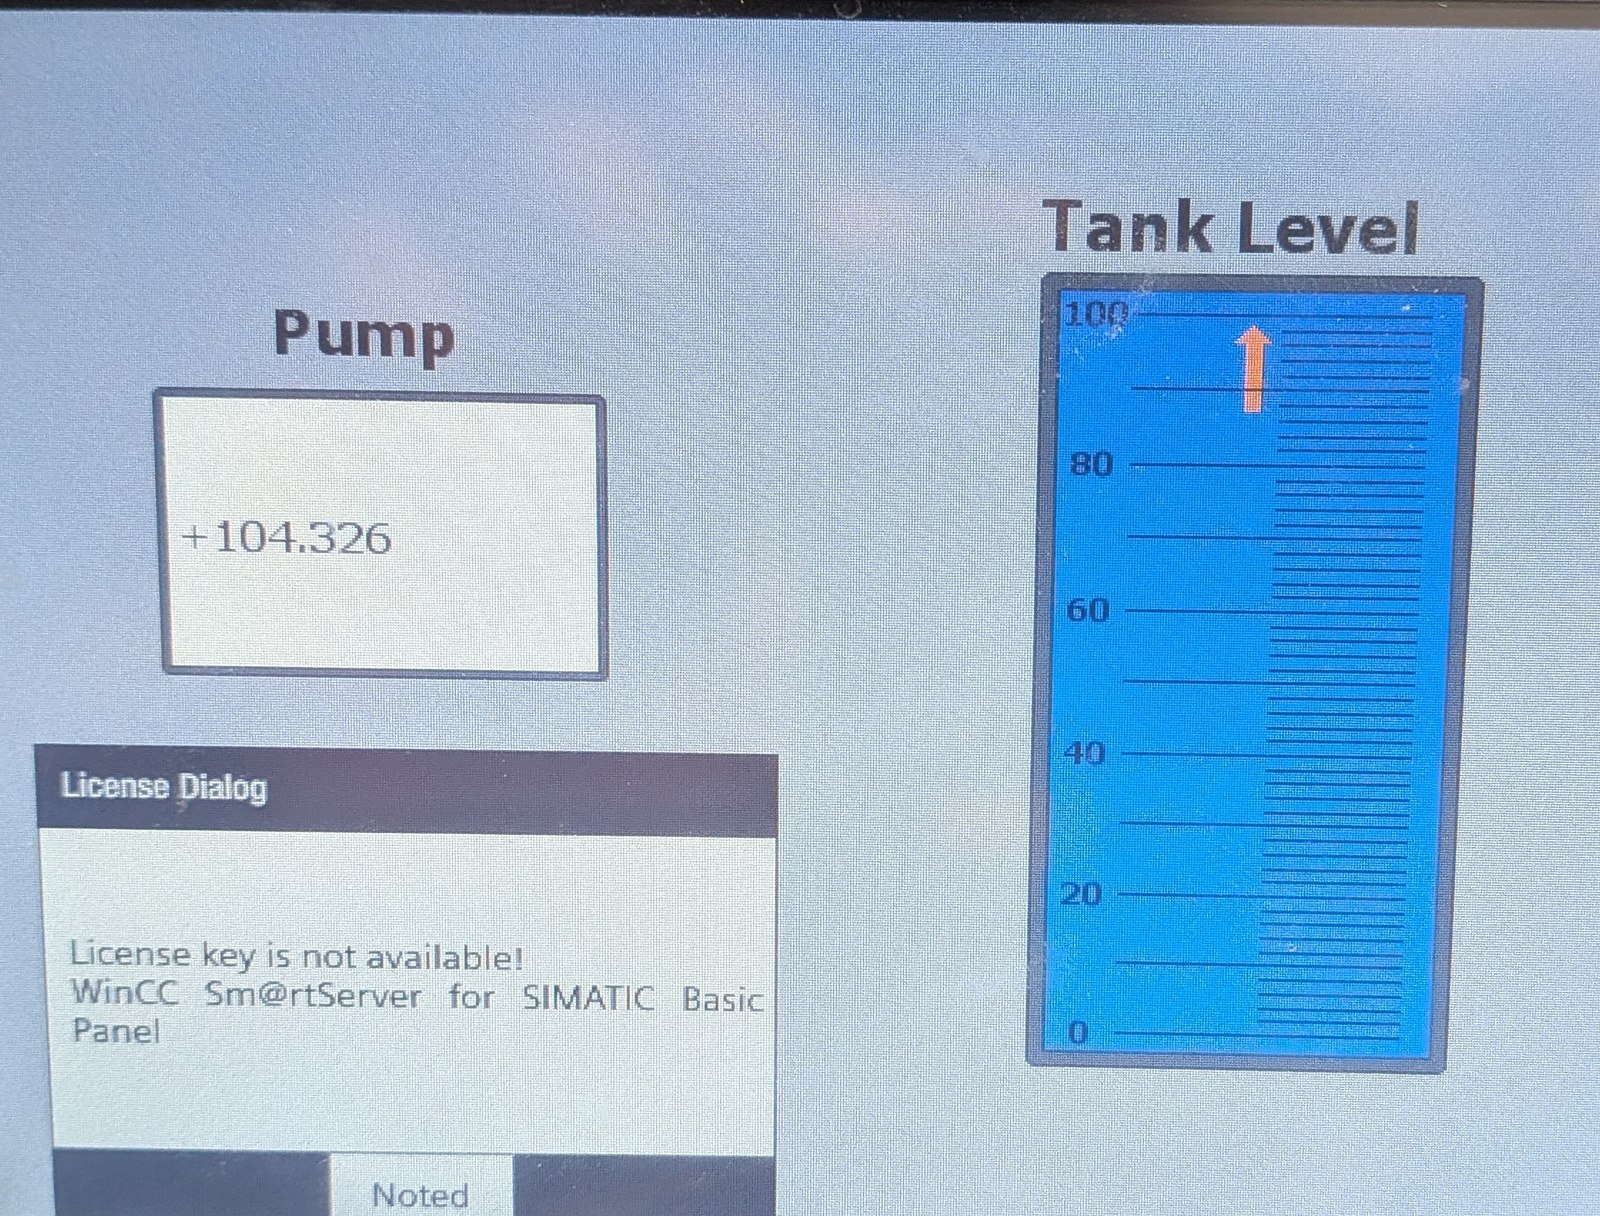
\includegraphics[width=\linewidth]{p6_overflow_hmi.jpg}\end{minipage}
\caption{Process devastation, disarmed. Left: the Factory IO tank driven full and over the top. Right: the operator panel at the same moment, the level cresting past the full mark at \texttt{+104.326} with the high-level alarm raised. The attacker holds the process out of its safe band and the operator cannot recover it.}
\label{fig:p6overflow}
\end{figure}

Armed, the same attack is severed before it can move the process. The injection's writes are CONTROL operations to the CRITICAL PLC1; CARS classifies them FORBIDDEN and isolates the source. The attacker's client cannot commit a single write: its S7 session times out before the first write lands, so zero writes reach the PLC, and a second attempt cannot even open a connection, its traffic already dropped. The enforcement is a real installed rule, not a log entry. On every switch the controller installs \texttt{cookie=0xca}, \texttt{table=1}, \texttt{priority=110}, \texttt{nw\_src=192.168.2.31}, \texttt{actions=drop} with a 75-second self-healing timeout, the CRITICAL duration (Figure~\ref{fig:p6armedflow}); the controller's own decision log shows the same event across the layer as a \texttt{FORBIDDEN~$\Rightarrow$~ISOLATE~(ENFORCED)} verdict on \texttt{192.168.2.31} (Figure~\ref{fig:dashisolate}), and the rule self-expires after its 75-second window. With no write reaching the PLC the tank never leaves its band and the process stays under the PLC's control. This is block-and-maintain: the attack is severed at the datapath before it can move the process. The dashboard itself, how it discovers the topology from the controller and renders each live decision, is described in Appendix~\ref{appx:dashboard}.

\begin{figure}[t]
\centering
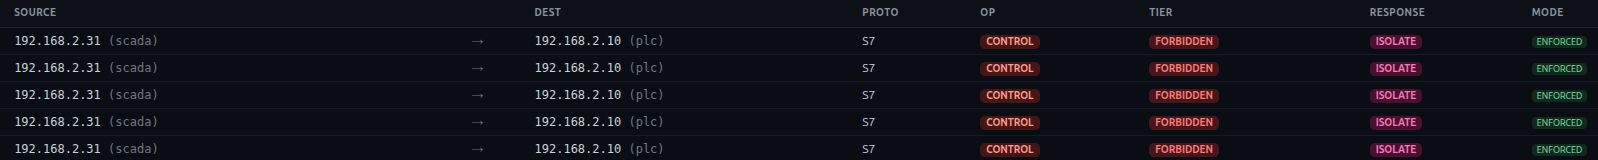
\includegraphics[width=0.98\textwidth]{dash_decisionlog.png}
\caption{The same armed isolation seen at the decision layer on the CARS dashboard: the compromised supervisory host \texttt{192.168.2.31 (scada)} issuing S7 CONTROL to the CRITICAL PLC1 is classed FORBIDDEN and met with an ENFORCED ISOLATE. This is the cross-layer counterpart to the datapath rule of Figure~\ref{fig:p6armedflow}: the same event as a policy decision rather than an installed flow.}
\label{fig:dashisolate}
\end{figure}

\begin{figure}[t]
\centering
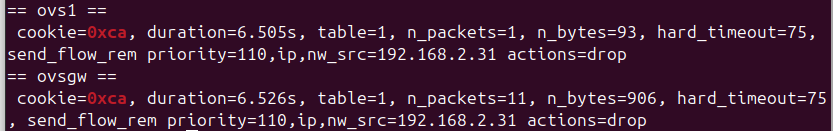
\includegraphics[width=0.95\textwidth]{p6_armed_flow.png}
\caption{Armed enforcement at the datapath. The reactive source-quarantine rule installed on \texttt{ovs1} and \texttt{ovsgw} in response to the injection: \texttt{cookie=0xca}, \texttt{priority=110}, \texttt{nw\_src=192.168.2.31}, \texttt{actions=drop}, \texttt{hard\_timeout=75}. The non-zero packet counters are the attacker's own traffic being dropped; the rule self-expires after 75\,s.}
\label{fig:p6armedflow}
\end{figure}

The contrast is stark on both the network and the process (Figure~\ref{fig:p6compare}). The identical FDI injection, sourced from the compromised supervisory host \texttt{192.168.2.31} and run over a matched forty-second window, landed 973 writes at the PLC disarmed against none armed; disarmed the tank crested past the full mark and overflowed, the process consequence of an unblocked injection shown in Figure~\ref{fig:p6overflow}, and armed it stayed within its safe band. The armed zero is not a near miss but a clean severance: the source is classified FORBIDDEN and isolated before its S7 session commits a single write.

\begin{figure}[t]
\centering
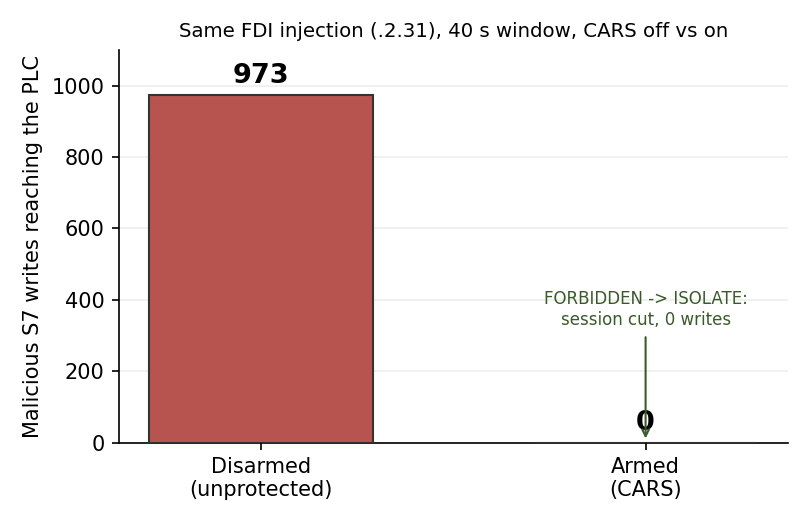
\includegraphics[width=0.6\textwidth]{chart_armed_vs_disarmed.png}
\caption{The same FDI injection from the compromised supervisory host \texttt{192.168.2.31}, run over a matched forty-second window with CARS disarmed then armed: malicious S7 writes reaching the PLC, 973 disarmed against 0 armed. Armed, the source is classified FORBIDDEN and isolated before its S7 session commits a write. Measured from the injection runs and the controller decision log.}
\label{fig:p6compare}
\end{figure}

\subsection{The rest of the repertoire}
\label{sec:evalrepertoire}

The remaining vectors ran in the same armed session, captured at the three wire points. Against the control plane, an unauthenticated request to disarm the defence, \texttt{POST /cars/defense \{on:false\}}, was refused with \texttt{HTTP 401} and logged as \texttt{DENIED (bad/missing token)}; CARS stayed armed, so a compromised control-plane host cannot silently switch the defence off. A flow tamper that injected a bogus rule and deleted a real conduit was caught by the flow-integrity checker within one ten-second poll, its verdict moving to \texttt{ok:0, missing:1, extra:1}, and cleared back to \texttt{ok:1} on restore without re-baselining, which shows the restoration was byte-exact. An out-of-state attack, forged ACKs from \texttt{192.168.2.66} to the PLC, did not reach it: the stateful table admitted none. And the operation-aware case, a compromised SCADA writing a bogus level to the PLC, was isolated on the write while the remediation agent restored the value, the level holding near 50 and the loop still running, the same block-and-maintain as the devastation phase. Through all of it the legitimate Factory IO loop and the historian telemetry were permitted, so the campaign carried no false positives from end to end.

The two external vectors close the campaign, driven from the Kali attacker \texttt{192.168.2.77}, the unregistered outsider of the threat model. Reconnaissance learned nothing under CARS: every scanned port on the PLC, including the S7 port 102, returned \texttt{filtered}, the \texttt{s7-info} probe drew no model or firmware, and the scan was reactively isolated. The controller logged the scan as \texttt{ISOLATE source 192.168.2.77 75s \dots ENFORCED [CRIT:CRITICAL]}, and the drop rule appeared on the switches as \texttt{cookie=0xca, priority=110, nw\_src=192.168.2.77}. Identity spoofing was dropped at the door: forging ARP as the trusted seam \texttt{192.168.2.31}, every forged frame was dropped at GUARD ingress and logged as \texttt{REFUSED (identity-spoof) - 192.168.2.31 impersonation dropped at GUARD ingress (dpid3)}, while the real seam kept flowing (Appendix~\ref{appx:scenarios}). The whole campaign is summarised in Table~\ref{tab:campaign}.

\begin{table}[t]
\centering
\small
\begin{tabular}{p{0.20\textwidth}p{0.36\textwidth}p{0.36\textwidth}}
\hline
Vector & Unprotected & Armed (CARS) \\
\hline
Reconnaissance & PLC ports open; model and firmware fingerprinted & all ports \texttt{filtered}; no S7 identity leak; scanner isolated \\
Identity spoofing & forged frames accepted as the trusted seam & 5/5 spoofed ARP dropped at GUARD ingress; real seams unaffected \\
State manipulation & out-of-state frames serviced by the PLC & none admitted by the stateful table \\
Control-plane disarm & defence silently switched off & refused (\texttt{HTTP 401}); stays armed \\
Flow tamper & injected and deleted rules persist & flagged by the flow-integrity checker within one poll; self-clears on restore \\
Operation-aware injection & bogus writes actuate the process & isolated on the write; remediation restores (block-and-maintain) \\
Process devastation & tank overflows to $\sim$104\%, alarm raised & isolated on the first write; datapath drop installed; tank held \\
\hline
\end{tabular}
\caption{The campaign, armed against unprotected. Every \emph{armed} outcome was captured live on 5 August, the external vectors from the Kali attacker \texttt{192.168.2.77} and the insider vectors from the compromised supervisory host \texttt{192.168.2.31}, corroborated by the controller decision log, the nmap and GUARD dumps, and the installed flows (Appendix~\ref{appx:scenarios}); the process-devastation contrast was re-captured fresh on the live tank (Section~\ref{sec:evaldevastation}). The two \emph{unprotected} reconnaissance and spoofing entries are the known flat-network baseline, an unenforced switch trivially serves a port scan and accepts a forged frame, and are given as reference rather than as a fresh measurement of our system. The legitimate Factory IO loop and historian telemetry were permitted throughout, so the campaign held zero false positives.}
\label{tab:campaign}
\end{table}

\section{Cross-layer validation}
\label{sec:evalcrosslayer}

A decision log can be doubted; independent agreement across every layer is harder to dismiss. A deep end-to-end trial drove the full response spectrum through the real autonomous chain and recorded, for each scenario, five independent layers: the packet on the Snort mirror, the Snort alert, the controller's decision, the installed OpenFlow rule, and the outcome at the client. Table~\ref{tab:crosslayer} gives the result; at every rung the layers tell the same story.

\begin{table}[t]
\centering
\small
\begin{tabular}{lllll}
\hline
Response (trigger) & Snort & CARS tier & OVS enforcement & Outcome \\
\hline
REFUSE (HMI loop) & n/a & CRITICAL & none installed & loop runs \\
ALLOW (READ FC3) & +283 & OPERATIONAL & none & read returns \texttt{[101..104]} \\
THROTTLE (WRITE FC6) & +285 & SENSITIVE & meter, p100 & write rate-limited \\
BLOCK (attacker WRITE) & +420 & FORBIDDEN & drop, p100 & connect fails \\
ISOLATE (persistence) & alert & FORBIDDEN & \texttt{0xca} src-drop, p110 & source cut \\
DEFLECT (policy) & alert & FORBIDDEN & \texttt{0xca} redirect, p105 & sent to honeypot \\
default-deny (bypass) & none & silent & A2 pre-drop & connect fails, no window \\
\hline
\end{tabular}
\caption{Cross-layer proof from the deep end-to-end trial: each response, with the Snort alert delta, the controller tier, the installed OpenFlow rule, and the client outcome. The last row is the proactive default-deny with the detection bridge off, showing a drop with no Snort or controller involvement and therefore no reaction window.}
\label{tab:crosslayer}
\end{table}

The DEFLECT row was probed further to see whether the deception actually engages. Forcing DEFLECT on the attacker's conduit installs the redirect, a priority-105 rule rewriting the destination to the honeypot, and a fresh capture at the decoy confirmed the diversion on the wire: the attacker's packets to the CRITICAL PLC arrived instead at the honeypot \texttt{192.168.3.99}, which began to answer, while the real PLC saw nothing. The full interactive round-trip, the decoy sustaining a two-way session so the attacker receives spoofed replies, did not complete in testing, because the minimal decoy could not resolve the attacker's address across the deception boundary; a production interactive honeypot is future work. The value demonstrated is the one that matters for protection: DEFLECT moves the attacker off the real asset and onto the decoy (Appendix~\ref{appx:gapevidence}).

The sharpest single proof is at the packet level. In the S7 write attack on PLC1, the attacker's Write-Var frames were counted at two capture points, the Snort mirror (what the detector sees) and the PLC's own port (what actually arrives). Armed, the mirror saw eight write attempts but only one reached the PLC, the single reaction-window leak, and the other seven were dropped in the fabric; disarmed, seven of the eight reached the PLC (Table~\ref{tab:wiredrop}). The drop is shown on the wire, not inferred from a log. The size of this leak depends on where the reaction window falls against the S7 handshake: in the matched forty-second injection of Section~\ref{sec:evaldevastation} the isolate landed during session setup, so no write committed at all, whereas here it fell one write later. In both the leak is at most a single write, and in neither did the process move.

\begin{table}[t]
\centering
\begin{tabular}{lcc}
\hline
S7 Write-Var frames (\texttt{.31$\to$.10}) & at Snort mirror & reached PLC \\
\hline
Armed & 8 & 1 \\
Disarmed & 8 & 7 \\
\hline
\end{tabular}
\caption{The drop shown on the wire. Attacker S7 Write-Var frames counted from the pcaps at the two capture points. Armed, eight are seen by the detector but seven are dropped in the fabric and only one leaks through in the reaction window; disarmed, seven of eight reach the PLC.}
\label{tab:wiredrop}
\end{table}

The same two captures make the drop visible frame by frame (Figure~\ref{fig:wireproof}). At the mirror the attacker's writes appear at frame 1348 (\texttt{t+6.380\,s}) and 1415 (\texttt{t+6.691\,s}); at the PLC port only the first, frame 1374 (\texttt{t+6.380\,s}), arrives. The isolate installed in the intervening third of a second, so every write from 6.691\,s on is seen by the detector but never reaches the PLC. The operation CARS acts on is read straight from the frame (Figure~\ref{fig:s7frame}): a Write Var to the output area, an actuation.

\begin{figure}[t]
\centering
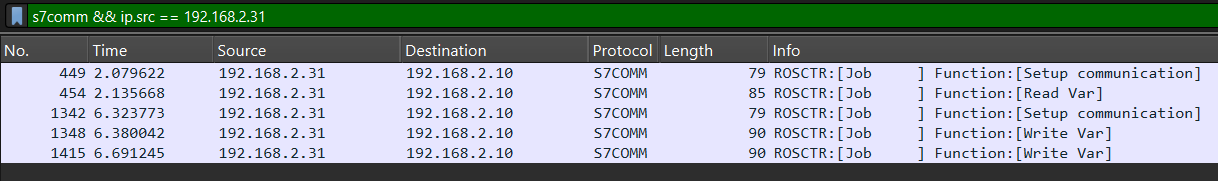
\includegraphics[width=\textwidth]{wire_armed_mirror.png}\\[4pt]
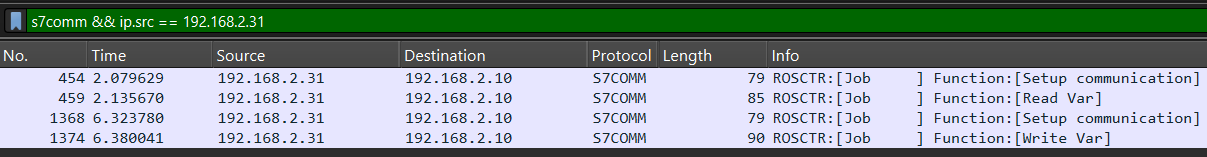
\includegraphics[width=\textwidth]{wire_armed_plc1.png}
\caption{The drop on the wire, armed, the S7 conduit filtered to the attacker (\texttt{s7comm \&\& ip.src==192.168.2.31}). Top, at the Snort mirror: the write frames are seen (1348 at \texttt{6.380\,s}, 1415 at \texttt{6.691\,s}). Bottom, at the PLC port: only the first write (1374 at \texttt{6.380\,s}) arrives; every later write is dropped in the fabric.}
\label{fig:wireproof}
\end{figure}

\begin{figure}[t]
\centering
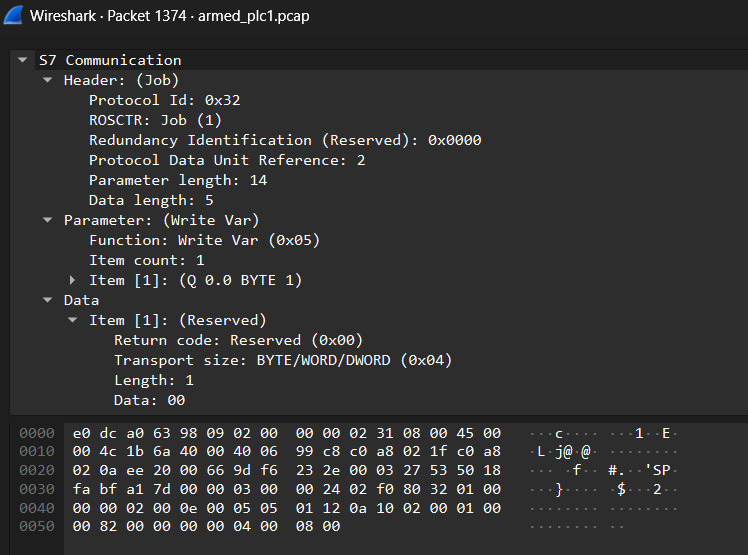
\includegraphics[width=0.68\textwidth]{wire_s7_writevar.png}
\caption{The malicious operation on the wire (frame 1348). CARS recovers the operation from the S7 parameter, \texttt{Function: Write Var (0x05)} to \texttt{Area: Outputs (Q) (0x82)}, an output actuation, and classifies it as CONTROL, forbidden on the CRITICAL PLC.}
\label{fig:s7frame}
\end{figure}

\subsection{Operation-awareness at the wire}
\label{sec:evaldpi}

CARS decides on the industrial operation recovered from the packet, not the five-tuple. Firing the operation spectrum from one trusted operator (\texttt{192.168.2.31}) at the Modbus unit, the same conduit draws a different verdict per function code (Table~\ref{tab:dpi}): a read passes, a write is throttled, and the dangerous operations are forbidden. The wire confirms the discriminator directly, the identical conduit carried an FC\,03 (read) and an FC\,06 (write), the function code sitting at offset seven of the Modbus payload, and CARS allowed the first and throttled the second on that one byte.

\begin{table}[t]
\centering
\small
\begin{tabular}{lllll}
\hline
Operation & Modbus FC & CARS tier & Response & Detection \\
\hline
READ & \texttt{0x03} & OPERATIONAL & ALLOW & reliable \\
WRITE & \texttt{0x06} & SENSITIVE & THROTTLE & reliable \\
CONTROL & \texttt{0x05} & FORBIDDEN & BLOCK & reliable \\
DIAG & \texttt{0x08} & FORBIDDEN & BLOCK, then ISOLATE & sustained only \\
PROGRAM & \texttt{0x2B} & FORBIDDEN & BLOCK & unreliable \\
ILLEGAL & \texttt{0x64} & FORBIDDEN & BLOCK & intermittent \\
\hline
\end{tabular}
\caption{Operation-awareness on the same conduit. The tier and response are the policy, correct for every operation, as the decision matrix of Section~\ref{sec:evalaccuracy} establishes by driving each operation through the engine directly. The detection column records how reliably the Snort sensor recovers that operation from the wire.}
\label{tab:dpi}
\end{table}

The detection column records an honest limitation, and it is the one qualification on the operation-awareness claim. The classification is the policy, and it is correct for every operation. The sensor that recovers the operation from the wire, however, is not equally reliable across all of them. The common operations (read, write, control) are recovered reliably, and a sustained dangerous operation is caught and escalated (a repeated DIAG was blocked and then isolated). But a single crafted dangerous frame can evade the single-packet inspection, and the rarer Modbus function codes were detected only intermittently, the MEI program request slipped through a sustained run and the illegal-code family was caught only once. A dangerous operation the sensor fails to recognise is not classified, so it falls to the source's base tier and is permitted. Two distinct weaknesses sit behind this and they are treated differently. Intermittent recovery of the rarer function codes is a sensor-tuning limit that remains, carried into Section~\ref{sec:threats}. The sharper one, fragmentation, was closed. Because the deployed rules matched the operation byte at a fixed packet offset with no stream reassembly, an attacker on an already-permitted conduit could split an S7 write across two TCP segments so the function byte fell in the second, and the operation was never recovered. A fresh test from the allowlisted \texttt{192.168.2.31} confirmed it: a Write-Var fragmented at byte fourteen drew only \texttt{TCP => ALLOW}, no rule was installed and the write reached the PLC, whereas the identical write sent whole drew \texttt{FORBIDDEN => ISOLATE}. The fix has two parts, because reassembly alone was not enough: TCP stream reassembly was enabled for the S7 and Modbus ports, and the operation-class rules were re-anchored to the protocol header: the operation byte, previously matched at a fixed \texttt{offset:17}, is now matched PDU-relative as \texttt{distance:8; within:9} after the \texttt{32 01} S7 job header, so a reassembled PDU is recognised wherever it sits in the stream. Re-run against the same fragmented attack at two split points, the write is now recovered, classified FORBIDDEN and the source isolated, with the legitimate high-rate loop still permitted and no new false positive (Appendix~\ref{appx:code}; the before-and-after capture and the full rule diff, Listing~\ref{lst:ev_rulesdiff}, are in Appendix~\ref{appx:gapevidence}). This raises the bar rather than settling the evasion question: overlapping-segment and timing evasions remain a general IDS problem, and single-frame recognition of the rarest codes is still imperfect. The annotated frame breakdowns at the three wire points, the S7 and Modbus function bytes read off the wire and the armed-versus-unprotected captures are collected in Appendix~\ref{appx:wire}.

\section{Reaction window and latency}
\label{sec:evallatency}

The decision itself is close to free. The controller reports a mean decide-and-enforce time of 0.027\,ms over the campaign (Figure~\ref{fig:status}), so classifying an operation and selecting its response adds nothing measurable to the path. The cost that matters for a reactive defence lies elsewhere, in the reaction window: the interval between an attack reaching the wire and the reactive rule landing in the switch, during which a few packets can still reach the target.

The armed process-devastation run bounds the window at the process level: the attacker's client could not commit a single write, the isolate cutting its S7 session before the first write landed, so zero writes reached the PLC against the 973 it managed disarmed, and a second connection moments later could not open at all. The source was quarantined for 75 seconds and the tank never left its band. The window itself is measured directly, not inferred from this run, by the harness below.

A dedicated harness times the window directly, measuring attack-frame-to-enforcement on a single clock. Over one hundred autonomous trials the median mitigation was 7.6\,ms, with a 95th percentile of 38.4\,ms and a 99th of 67.9\,ms; the fastest of the hundred was 5.5\,ms and the slowest 72.9\,ms, and every trial ended in an ISOLATE (Figure~\ref{fig:mttmchart}). The distribution is a tight mode of a few milliseconds with a small upper tail, not a broad spread, and its shape has a mechanical explanation rather than being random jitter.

Timestamping each stage separates detection from the response that follows. Snort raises its alert on the attacking frame within a fraction of a millisecond of that frame reaching the mirror, so detection is effectively free; the whole window is the response path that follows, the bridge reading the alert, the post to the controller, the decision, and the flow-modification message reaching the switch, which together take a median of about 7.5\,ms. Because that path is near-constant the window clusters. The tail has a single cause: the bridge follows Snort's alert file on a fifty-millisecond cycle, so an alert that arrives just after a read waits up to one cycle before it is handled, which is why the slow trials sit near fifty to seventy milliseconds rather than scattering. The tail is a discrete polling boundary, in the same class as the flow-integrity poll, not network noise.

The window also tracks the load on the detection path. Across the hundred trials the reaction correlated with the volume of background alerts the bridge was processing, at a Pearson coefficient of $0.43$, and the tail trials carried a heavier background than those in the mode. That background is not small: the hardware-in-the-loop input alone drives about thirty-two industrial operations a second on this testbed, so the reactive path already competes with a steady alert stream. A heavier multi-source event would lengthen the queue at the file-tailing, HTTP-posting bridge and widen the window further; that bridge is the acknowledged bottleneck, and its remedy, in-memory inter-process communication, is carried in Section~\ref{sec:threats} and the future work. An attempt to load the detector from a single source did not widen it far, because the volumetric overlay throttles a flood before it can build, which is a bound worth noting in its own right.

To characterise that load ceiling directly, the deployed decision path was measured two ways. Driving the engine's own \texttt{classify} and \texttt{select\_response} code as a bench, the per-decision compute is a few microseconds, and the decision together with its audit-log write sustains on the order of sixteen to eighteen thousand alerts a second on a single core before the single-threaded stage saturates and latency grows. On the live testbed, sweeping a benign background decision load against a timed probe, the reaction window held at roughly eight to fifteen milliseconds up to about a thousand background operations a second, rising to about seventy milliseconds only under thirty-two simultaneous in-flight requests, which is head-of-line queueing at the single-threaded controller rather than throughput saturation, and not the serial path a rate-limited detection bridge actually presents. Two properties keep an attacker well below the ceiling: identical alerts are collapsed by the three-second cooldown to at most one event per source, conduit and operation, and a diverse flood is still bounded by the same throttle that governs the reactive path. The window therefore stays in the tens of milliseconds across any rate a real, de-duplicated attacker can offer, and lengthens only as the single-threaded controller nears saturation, which is exactly what the in-memory inter-process bridge of the future work is meant to raise.

These figures are for a single injection, the case that matters for a false-data attack that needs only one write to land. A sustained flood behaves differently: fired continuously from the Kali attacker virtual machine rather than a co-located namespace, an ICMP flood on the CRITICAL PLC was isolated within a median of about one second, leaking of the order of forty frames first. Those frames are inert layer-three probes that never reach the S7 process, and the tank cycled without disturbance throughout, so a single injection is cut in milliseconds and a sustained real-attacker flood in about a second, with what leaks in either case unable to move the process.

\begin{figure}[t]
\centering
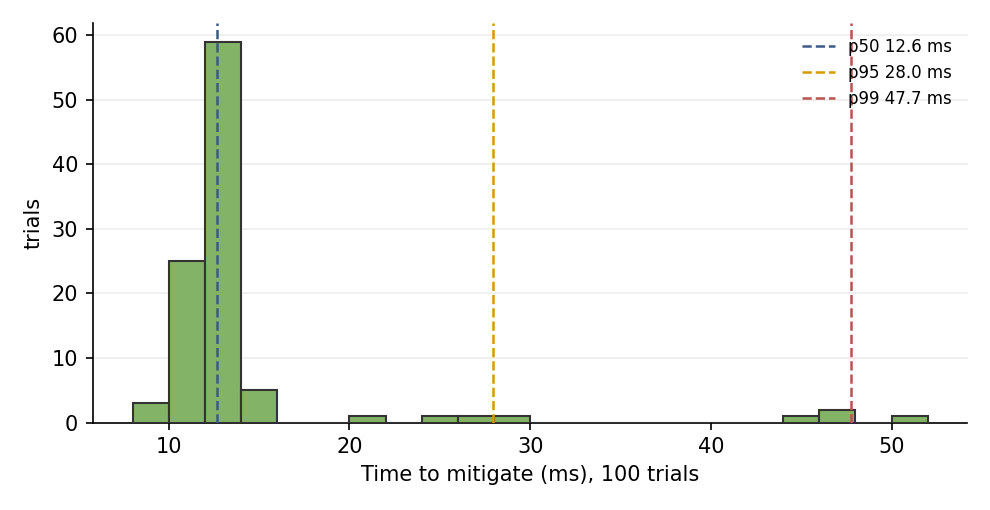
\includegraphics[width=0.82\textwidth]{chart_mttm.png}
\caption{Reaction window over one hundred autonomous trials, attack frame to enforcement on a single clock. Median 7.6\,ms, 95th percentile 38.4\,ms, 99th 67.9\,ms, maximum 72.9\,ms; every trial ended in an ISOLATE. The window is the detect-then-respond plumbing (Snort alert to installed flow); the upper tail is the bridge's fifty-millisecond alert-file poll boundary.}
\label{fig:mttmchart}
\end{figure}

This window is a property of any detect-then-respond defence, in the same class as the flow-integrity poll interval, not a defect to be removed: detection, decision and installation take a finite, small time. The defence's value is that the window is short, the leaked packets are inert, and the enforcement then holds and self-heals. Pre-empting every first packet is the job of a proactive layer, which is exactly what the identity binding, allowlist and default-deny of the pipeline provide for the conduits they cover; the reactive graded response governs what those static layers pass on to inspection.

\section{Anatomy of a defended attack: two pivots end to end}
\label{sec:evalanatomy}

The preceding sections measured CARS one property at a time. This section binds them into a single causal account: one attacker machine, driven from two network positions, with every stage of the defence followed on one clock from the launched packet to the installed flow and the operator's log. The value of the trace is that nothing is asserted in isolation: each claim about a rule, a decision or an enforcement is the next link in a chain that begins with a real frame captured on the wire.

The attacker is a single Kali virtual machine, dual-homed by design (Figure~\ref{fig:travelpath}). Its \texttt{eth2} interface (\texttt{10.0.40.66}) sits in the enterprise IT zone and reaches the process network only by routing north-to-south through the modelled perimeter: an Enterprise firewall, a DMZ, and an OT firewall that source-NATs every crossing onto the single gateway address \texttt{192.168.2.1}. Its \texttt{eth1} interface (\texttt{192.168.2.77}) sits directly on the OT segment as an unregistered host. The same tool, the same target and the same operation are launched from each; only the attacker's position changes. That isolates the one variable that matters for an identity-bound defence: whether the fabric can see who is really attacking.

\begin{figure}[t]
\centering

\includegraphics[width=\textwidth]{story_travelpath.png}
\caption{The two pivots from one Kali. \texttt{eth2} routes north and source-NATs to the gateway identity \texttt{192.168.2.1}; \texttt{eth1} sits on the OT segment as \texttt{192.168.2.77}. Both are quarantined at the gateway switch before a single packet reaches PLC1, but on different \texttt{nw\_src} identities.}
\label{fig:travelpath}
\end{figure}

Every packet that enters the fabric meets the same three-table pipeline (Figure~\ref{fig:carspipeline}). Table~0 (GUARD) binds each protected identity to its physical port and MAC and drops a forgery before it can reach policy. Table~1 (POLICY) passes an established connection, then an allowlisted conduit, then any reactive rule the controller has installed, and default-denies everything else. Table~2 forwards what survives. In parallel, the gateway switch mirrors traffic to Snort, whose alerts the bridge turns into an operation and a rate and posts to the controller, whose \texttt{classify()} and \texttt{select\_response()} decide a tier and a graded response and, when warranted, install a reactive drop stamped with cookie \texttt{0x00CA}. Three termination classes fall out of this pipeline: a spoofed identity dies at Table~0; a non-conduit source is default-denied and, on any attempt against the PLC, reactively isolated; and an allowlisted conduit that turns malicious is caught by the deep-packet inspection loop. The two pivots exercise the middle class; the false-data injection of Section~\ref{sec:evalcampaign} exercised the third.

\begin{figure}[t]
\centering
\includegraphics[width=\textwidth]{story_pipeline.png}
\caption{The CARS decision pipeline and where each attack class terminates. The two pivots (non-conduit sources) are cut at Table~1; the allowlisted insider is delivered one packet, then caught by the DPI loop that recovers the S7 operation and installs the \texttt{0x00CA} isolate.}
\label{fig:carspipeline}
\end{figure}

\textbf{Pivot A, the IT attacker.} The Kali opens an S7 session to \texttt{192.168.2.10:102} over \texttt{eth2}. The frame is routed through the perimeter and arrives at the gateway switch source-NATed: the mirror records \texttt{192.168.2.1.33440 > 192.168.2.10.102} with the SYN flag, preceded by an ARP for the PLC, so every northern host has collapsed onto the one gateway identity. The controller resolves \texttt{192.168.2.1} to the \texttt{gateway} role, finds no allowlisted conduit to the CRITICAL PLC1, and classifies the attempt FORBIDDEN; because the destination is CRITICAL the response is an immediate source isolation. The audit line reads \texttt{FORBIDDEN 192.168.2.1(gateway) -> 192.168.2.10(plc) TCP => ISOLATE source 192.168.2.1 75s [CRIT:CRITICAL]}, and a matching flow appears on both \texttt{ovs1} and \texttt{ovsgw}: \texttt{cookie=0xca, priority=110, nw\_src=192.168.2.1, actions=drop, hard\_timeout=75}. The consequence for the attacker is a TCP connect timeout with zero writes landed; the gateway rule absorbed the SYN retransmits (\texttt{n\_packets}=4 at \texttt{ovsgw}) and the PLC-side capture shows nothing reaching the process. The containment is total but, as first captured, \emph{coarse}: the quarantine was a source isolation on \texttt{192.168.2.1}, so it stopped this attacker and every other northern host alike, the NAT collapse leaving CARS no finer handle on identity. That coarse cut is itself a cost, a denial of service on the shared gateway conduit, and it prompted a refinement to the response selection: a shared, NAT-collapsed identity is now cut at the conduit rather than the source. Verified on the deployed engine, the same attempt from \texttt{192.168.2.1} now installs \texttt{cookie=0xca, priority=100, nw\_src=192.168.2.1, nw\_dst=192.168.2.10, actions=drop}, dropping only the PLC-bound flow while the gateway's other traffic is untouched by construction, whereas a true single host such as Pivot~B still draws the finer source isolation (Appendix~\ref{appx:gapevidence}). The residual limit is stated honestly: across a NAT, CARS cannot separate the rogue IT host from its legitimate neighbours on that one conduit, so full per-host attribution still needs the boundary firewall to carry the real source.

\textbf{Pivot B, the on-segment insider.} The identical S7 connection is launched from \texttt{eth1}, and now the mirror records the attacker's \emph{true} address: \texttt{192.168.2.77.42712 > 192.168.2.10.102} with the SYN flag. The controller resolves \texttt{192.168.2.77} to \texttt{unknown} (it is unregistered), again finds no conduit, and issues the same verdict, \texttt{FORBIDDEN 192.168.2.77(unknown) -> 192.168.2.10(plc) TCP => ISOLATE source 192.168.2.77 75s [CRIT:CRITICAL]}, but the installed flow now reads \texttt{nw\_src=192.168.2.77}. The attacker again gets a connect timeout and zero landed, but the quarantine is \emph{fine-grained}: it names the actual host, leaving every other OT identity untouched. Both pivots were severed at the TCP-connect layer: because neither is an allowlisted conduit, the connection to the PLC's control port is itself forbidden, so the handshake never completes and no S7 payload is ever emitted.

\begin{table}[t]
\centering
\small
\begin{tabular}{@{}p{3.1cm}p{5.0cm}p{5.0cm}@{}}
\hline
\textbf{Stage} & \textbf{Pivot A: IT attacker} & \textbf{Pivot B: insider} \\
\hline
Launch & S7 connect from \texttt{eth2} (\texttt{10.0.40.66}) & S7 connect from \texttt{eth1} (\texttt{192.168.2.77}) \\
Travel path & Ent-FW $\rightarrow$ DMZ $\rightarrow$ OT-FW (SNAT) $\rightarrow$ ovsgw & OT segment $\rightarrow$ vmnet2 $\rightarrow$ ovsgw ofport 12 \\
Seen on the wire as & \texttt{192.168.2.1} (gateway, collapsed) & \texttt{192.168.2.77} (true host) \\
Rule matched & no conduit; default-deny & no conduit; default-deny \\
Decision & \texttt{gateway$\rightarrow$plc} FORBIDDEN & \texttt{unknown$\rightarrow$plc} FORBIDDEN \\
Response & ISOLATE 75\,s [CRIT:CRITICAL] & ISOLATE 75\,s [CRIT:CRITICAL] \\
Flow installed & \texttt{0xca nw\_src=192.168.2.1} (ovs1+ovsgw) & \texttt{0xca nw\_src=192.168.2.77} (ovs1+ovsgw) \\
Wire effect & connect timeout, 0 landed & connect timeout, 0 landed \\
Observability & audit + dashboard ISOLATE row & audit + dashboard ISOLATE row \\
\hline
\end{tabular}
\caption{The same attack, two positions, followed through nine stages. Enforcement is identical; the granularity of the quarantine is not.}
\label{tab:eventtrail}
\end{table}

Table~\ref{tab:eventtrail} lays the two traces side by side. The enforcement is identical in kind, tier and duration; the single difference is the identity CARS can act on, and that difference is the argument for pushing enforcement onto the segment. A perimeter defence sees only \texttt{192.168.2.1} and must treat the whole enterprise as one suspect; CARS on the OT fabric names \texttt{192.168.2.77} and quarantines exactly it. Neither attacker moved the process, but only the on-segment case could be attributed.

These two pivots are stopped before they can speak S7 at all. The third termination class, an \emph{allowlisted} conduit that turns malicious, is where the operation-aware machinery is exercised, and it was captured in the false-data injection of Section~\ref{sec:evalcampaign}: the compromised supervisory host holds a legitimate conduit, so its first write reaches the PLC (first-packet reality), the DPI loop recovers the S7 operation as a CONTROL write, and only then does the controller classify it FORBIDDEN and isolate the source while the remediation agent restores the process. Read together, the three cases are the whole of CARS: identity and conduit gating for who may connect, deep inspection for what an authorised party then does, and one graded, self-healing response mechanism behind both.

Placing the timing on this story closes it (Figure~\ref{fig:sequence}). In each pivot the first SYN was seen once and the isolate was installed within the reaction window characterised in Section~\ref{sec:evallatency}: a median of 7.6\,ms, 67.9\,ms at the 99th percentile. The attacker's own TCP stack did not retransmit until roughly one second later, by which time the drop was already in place: the defence closed roughly two orders of magnitude faster than the attacker could send its next packet, which is why the wire shows one SYN seen and the rest absorbed. The reaction window is real, but on this evidence it is far shorter than the interval over which even an automated attacker operates. Equally, the decision at the heart of each trace is not a one-off: the \texttt{classify()} verdict that both pivots received is the same rule evaluated, without error, across the scored matrix and the exhaustive decision domain of Section~\ref{sec:evalaccuracy}, so each trace is one observed instance of a rule whose correctness is quantified with a confidence interval rather than asserted from a single run.

\begin{figure}[t]
\centering
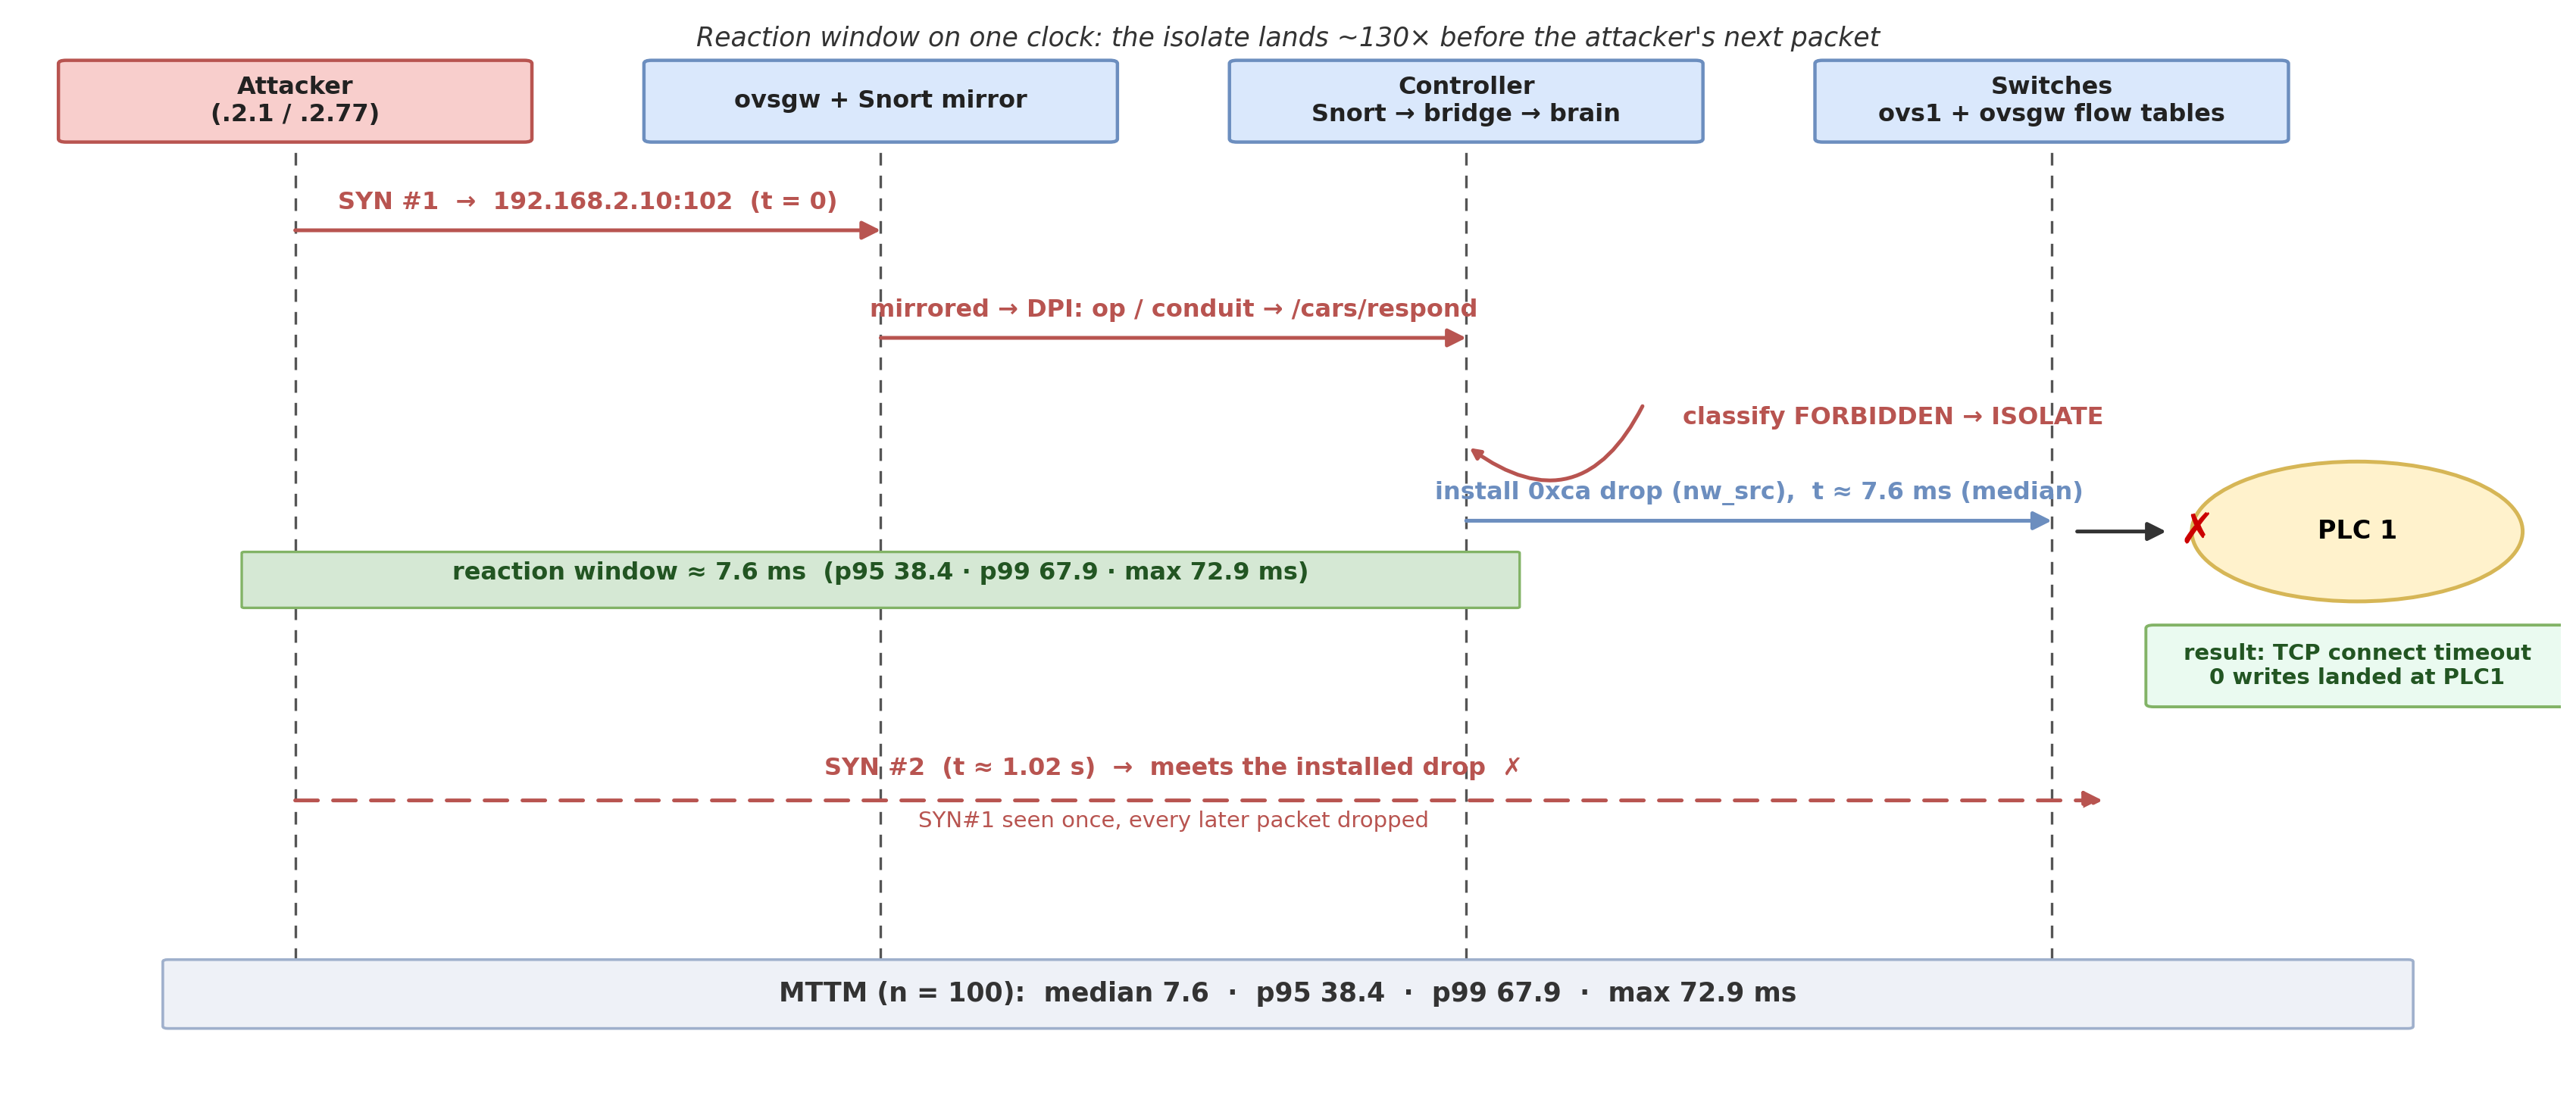
\includegraphics[width=\textwidth]{story_sequence.png}
\caption{The reaction window placed against the attacker's packet cadence. The \texttt{0x00CA} isolate lands within the measured mean-time-to-mitigate (median 7.6\,ms), while the attacker's TCP retransmits arrive $\sim$1\,s apart, so the first SYN is seen once and every later packet meets the installed drop.}
\label{fig:sequence}
\end{figure}

\section{Does the defence disturb the process?}
\label{sec:evalprocessrisk}

A defence for a live plant is deployable only if arming it does not perturb the process it protects. Two measurements answer this: the process under the armed pipeline with no attack, and the process while the defence actually fires.

Under normal operation the armed and disarmed fabric are indistinguishable at the process. No reactive rule is installed while nothing is detected, so the datapath a legitimate packet crosses is identical with enforcement on or off, and any difference would have to come from the pipeline itself. Interleaving the two states in short blocks over two hours under matched load, so that any drift in the hardware-in-the-loop simulation falls on both equally, the tank held the same band and spread in each: a mean level of 51.5\% disarmed against 50.7\% armed, standard deviations of 12.8 and 13.2, and no excursion beyond the control band in either, across seven thousand per-second samples, with legitimate throughput unchanged (Appendix~\ref{appx:availability}). Arming the defence has no measurable effect on the process. This result is established for the testbed and its hardware-in-the-loop tank, not for industrial processes in general: it shows that arming the pipeline did not perturb this live process, not that arming is harmless on every plant, since a faster or more tightly coupled loop could respond differently to the same enforcement machinery. A first, naive comparison of one armed hour against one disarmed hour was discarded when the simulation host stalled part way through and skewed the armed hour; the interleaved, load-matched method was adopted precisely to control for that, and it is why the result can be stated cleanly rather than as a difference confounded by drift.

When the defence does fire, it holds the process rather than harming it. A compromised but allowlisted supervisory host launched a false-data injection at the CRITICAL PLC under the armed defence: CARS classified the write FORBIDDEN and isolated the source after nine packets, the reactive drop carrying the criticality-scaled seventy-five-second timeout. For the whole of that block the tank stayed within its band with no excursion, the legitimate conduits kept flowing without interruption, and the restoration agent was never called, because the cut came fast enough that no physical anomaly developed. The rule then self-healed: it expired at its timeout, the source returned to service with no operator action, and the flow table returned to its baseline, the install-to-withdrawal spanning seventy-six seconds. This is the block-and-maintain property measured at the process rather than the wire: the attacker is severed, the plant is held, and the network heals itself without a human in the loop. The nine-packet cut is specific to this attack and this load, not a general guarantee; how the same bound behaves under mixed background traffic, bursts and TCP retransmissions, or a heavier controller load was not measured here and is a question for a larger trial.

\section{Process-layer defence in depth}
\label{sec:evalguardian}

The evaluation so far concerns the network: who may reach an asset, and with which operation. A separate question is what happens when the attacker is a genuinely trusted, allowlisted party acting within its permitted operations, the compromised engineering station or the corrupted agent behind classic ICS incidents. The network layer, by design, must not cut such a party on the critical path, so the natural worry is that a trusted insider drives the process to harm unchecked. Probing this on the live tank narrowed the concern before it justified a new layer.

The high-rate route is already covered. Driving the tank over its limit means spoofing the level sensor faster than the hardware-in-the-loop refreshes it, so the injection is necessarily high rate; when the trusted remediation identity \texttt{192.168.2.45} was used to run exactly that overflow, the volumetric overlay classified it a flood and cut the conduit after seventy-seven writes, the tank peaking in the mid-seventies rather than overflowing. Reading the PLC program confirmed there is no slow path to the same end: the fill thresholds are constants in the control block, the \texttt{Setpoint} input word is not referenced, and the level is recomputed from the sensor every scan, so a single low-rate write cannot re-aim the process. The rate overlay therefore closes the overflow that the network gating leaves to it.

Two residuals remain, both narrower and both real. The first is a low-rate authorised action: a trusted role issuing one legitimate command that is individually valid yet operationally harmful. The second is a blind spot inside the existing process agent, whose tamper test (Appendix~\ref{appx:code}) checks only the low side, a reading below a floor or a sudden fall, so it restores a sensor spoofed downward but ignores a reading driven high. To cover these a small process guardian was added as a defence-in-depth layer. It is a standalone, read-only Python monitor, separate from the SDN controller and its engine, that reads the tank level from the remediation agent's status feed and alarms on a high-side envelope breach, an impossible rate of change, or a stall in the level while the process should be cycling. Detecting attacks by checking the physical process against its expected invariants, rather than inspecting the network, is an established direction in control-system security \cite{cardenas2011attacks}; the guardian applies that idea as a narrow, alarm-only backstop to the response system. It never writes the PLC and never touches the enforcement or the remediation agent, so it cannot disturb the running system; it reports, and the network layer keeps its hands off the safety loop.

Both residuals were then exercised live. A trusted \texttt{192.168.2.45} issuing a single authorised HMI stop was permitted by CARS, correctly for an authorised control, and the process halted with the tank frozen at 40.4\%; the guardian raised a stall alarm twelve seconds later, catching a denial the network layer allows by design. Separately, with the reported level pinned high at 90\% (the reported-full deception, the real tank draining beneath it), the existing agent stayed silent, its low-side test blind to the excursion, while the guardian raised a high-level and a rate alarm on the same reading. The guardian catches what the network layer must not act on and what the low-side agent misses, without changing either. These are narrow, live demonstrations that the guardian catches cases the lower layers miss, evidence that the layer has a role, not proof that it is sufficient against a sophisticated covert manipulation. The guardian alarm feed, and the flood block that cut the runaway trusted identity, are collected in Appendix~\ref{appx:gapevidence}.

This does not claim to solve the insider problem. A manipulation that stays inside the physical envelope and moves the process slowly and plausibly evades an invariant monitor as it evades the agent, and the guardian is detection, an alarm to the operator, not prevention, because automating prevention on the safety loop is the risk this whole approach avoids. That the guardian only alarms is a deliberate boundary rather than a shortfall: it is the same operator-trust logic that runs through the whole design, since the reason the network layer must not cut the safety loop is the reason a process monitor must not act on it either, and a backstop an operator can leave armed is worth more than an automated action on the process that the operator would switch off. Moving from an alarm to a bounded, non-safety-loop action, for instance triggering the existing remediation agent's safe-value restore on a clear envelope breach, is a defensible next step and is carried as future work. What the layer buys is a clean division of responsibility: the network stops who and what should never connect, the rate overlay stops the high-rate abuse, and a process-invariant monitor makes the residual physical anomalies visible. The remaining stealthy-in-envelope case is carried to Section~\ref{sec:threats} and the conclusion as future work.

\section{Comparison with related work}
\label{sec:evalcompare}

CARS sits within the body of work on software-defined response for industrial networks, and its contribution is clearest against that work's known limits. Surveys of reactive SDN defence for ICS observe that most systems respond uniformly, dropping or redirecting a flagged flow regardless of what the flow was doing or how important its target is \cite{etxezarreta2023survey}. CARS decides instead on two axes, the industrial operation recovered from the packet and the criticality of the asset, so the same forbidden control draws a 75-second quarantine on the CRITICAL PLC and a 30-second block on the LOW-value unit, and a read from a source is allowed where a write from it is refused. The evaluation shows this grading changes the measured response tier by tier (Section~\ref{sec:evalcriticality}), rather than being cosmetic.

The self-checking layer relates to the policy-verification work of Melis et al.\ \cite{melis2018policychecker}, which checks the consistency of installed flow rules; the CARS flow-integrity checker performs the same class of check against a trusted baseline and, in the campaign, caught an injected rule and a deleted conduit within one poll. The threat it defends, a control-plane host that rewrites the fabric, is the one identified by Gardiner et al.\ \cite{gardiner2021controller}; CARS adds an authenticated control interface so the defence cannot be silently disarmed, which the campaign confirmed with the refused \texttt{HTTP 401}. The stateful shield in the pipeline follows the data-plane connection-tracking idea of AvantGuard \cite{shin2013avantguard}, and the replica-and-deception direction of Etxezarreta et al.\ \cite{etxezarreta2026replica} is an alternative to the CARS block-and-maintain, trading a decoy for a graded cut.

What separates CARS from the SDN-response systems it builds on, including the intrusion-response design of Samanis \cite{samanis2025phd}, is the deployment barrier it targets. The reactive defences in the literature are attractive but largely undeployed on live OT, because an over-eager block can cut the process; the central result here is a 0\% false-positive rate on the live process traffic with a bounded, reversible, evidence-generating response. That property, more than raw detection, is what an operator needs before a reactive defence can be armed on a running plant.

\section{Threats to validity}
\label{sec:threats}

The results are honest within limits that should be stated plainly. This is a functional-prototype validation on a single testbed with one process, not a product trial. The accuracy is exact over the twenty-four scored cases and is corroborated by the campaign's live decisions, but twenty-four scored permutations on one bench cannot guarantee a zero false-positive rate on a large, noisy production network; that would need a far larger and more varied traffic sample. The result should be read as: on this system and its rulebook, across the decision space and the live campaign, no legitimate operation was wrongly cut, and not as a statistical guarantee for arbitrary industrial traffic. The physical process is a hardware-in-the-loop: the PLC, the S7 traffic, the control logic and the enforcement are all real, but the water is simulated in Factory IO, so the overflow is a faithful process consequence rather than a spill of real fluid.

The reaction window deserves a sharper caveat than a general remark. Over a hundred trials the median mitigation was 7.6\,ms and the 99th percentile 67.9\,ms for a single injection, while a sustained flood fired continuously from the real attacker virtual machine was cut in about one second. On this slow tank that second is harmless; on a fast process, high-speed manufacturing or an electrical protection loop, one second is ample time for physical damage, and the reactive layer alone would not suffice there. The mitigation is architectural: the proactive layer, identity binding, allowlist and default-deny, drops a non-conduit or spoofed packet with no reaction window at all, so the residual exposure is a novel operation on an already-permitted conduit. This distinction bounds the pipelined-burst worry: an unregistered attacker never gets a window, because the default-deny stops it at the TCP handshake before any payload lands (the two pivots of Section~\ref{sec:evalanatomy} landed zero writes), so a burst of malicious writes inside the window is only possible from a compromised but allowlisted host, where the first packets reach the PLC by design and the injection of Section~\ref{sec:evalcampaign} landed nine before the cut. A short pre-isolation burst on such a conduit is therefore the true residual, narrowed by pushing more coverage into the proactive layer and closed at the endpoint only by a TCP reset on quarantine, both carried in the future work. Narrowing it further is a matter of pushing more coverage into the proactive layer or shortening the detection poll, and a fast process would demand both. The figure also reflects this attacker's cadence and the testbed's single-controller path: the injection client sends well below line rate and the control path carries no competing controller load, so the window measured here is a partial proxy for a production plant under concurrent traffic, scheduling jitter or multi-controller pressure, where queueing on the detection path would widen it, as the load correlation of Section~\ref{sec:evallatency} already begins to show.

A second limit is in the detection sensor, not the policy. The reactive layer depends on Snort to recover the operation from the packet. An earlier configuration inspected single packets at fixed offsets, which let a fragmented operation on an already-permitted conduit evade recognition; that specific gap was closed by enabling stream reassembly and re-anchoring the rules to the protocol header (Section~\ref{sec:evaldpi}), and a fragmented write is now recovered and blocked at more than one split point. What remains is narrower: the rarest Modbus function codes are still recognised only intermittently, and a sufficiently crafted overlapping-segment or timing evasion is a general IDS problem this work does not claim to settle. The decision logic classifies every operation correctly once it is known, so this is a sensor-coverage limit rather than a flaw in the response, and sharpening the sensor's protocol parsing further is future work. Enabling stream reassembly to close the fragmentation gap does add state to the sensor, which a reassembly-targeted session flood could try to exhaust; that state is bounded on this deployment (\texttt{max\_tcp 8192} sessions, sixty-second timeout), and because the sensor runs on a passive mirror rather than inline, exhausting it degrades detection rather than stalling forwarding, since the proactive rules live in the switches independently of the sensor. The consequence of a sensor overload is therefore a loss of operation-awareness on allowlisted conduits, not a halted process, and per-source metering on the mirror is the further mitigation. A deeper limit sits underneath this: the operation-awareness depends on a readable payload. The classic S7comm and Modbus/TCP of this testbed carry the function in clear, but modern industrial protocols that encrypt or integrity-protect the payload, such as S7CommPlus on newer Siemens firmware, OPC UA with security enabled, or CIP Security, would deny the sensor the operation byte altogether. Under such a protocol the operation-aware reactive tier degrades to what can be judged without the payload, while the proactive stateful layer, the identity binding, the role and conduit allowlist and the default-deny, and the process guardian still hold; recovering operation-awareness there would need endpoint or host-based operation telemetry, or a protocol-aware proxy that terminates the secure session, both beyond this work.

Several further limits are architectural rather than defects in the decision logic, and they mark where a lab prototype stops short of a hardened deployment. The OpenFlow control channel runs in plaintext (\texttt{tcp:6653}), so an attacker who reached the control plane could intercept or forge flow rules; that plane is a separate wired management network (\texttt{10.10.10.0/24}) which none of the evaluated attackers can reach, so the exposure is bounded on this testbed. Relying on segmentation alone is nonetheless a weak posture for a centralised controller: a misconfiguration, a VLAN-hopping technique, or an engineering station dual-homed onto both the operational and management planes would defeat it, leaving the channel open to the control-plane interception and rule-forgery set out in Section~\ref{sec:controlplane} \cite{gardiner2021controller}. The proper mitigation is to run OpenFlow over TLS; this prototype does not implement it, and does not measure its latency overhead. The flow-integrity checker polls every ten seconds, which bounds but does not close its window. A fresh thirty-trial test of each case quantified this: a persistent injected rule was caught on every trial, thirty of thirty, at a median of 8.5\,seconds, whereas a rule injected and withdrawn inside a two-second window evaded the auditor on twenty-five of thirty trials, caught only on the five occasions its life happened to straddle a poll boundary (Appendix~\ref{appx:gapevidence}). Polling has an inherent blind spot below its interval, so an event-driven flow-monitor was built to close it: subscribing to the switch's Nicira flow-monitor, it checks every change to the policy tables against the trusted baseline the instant the change is installed, rather than sampling every ten seconds. Re-running the same thirty-trial transient test with the monitor active, the two-second injection was caught on every trial, thirty of thirty, at a median of 0.27\,seconds, against five of thirty for the poll, closing the sub-poll gap on the deployed OpenFlow stack (Appendix~\ref{appx:gapevidence}). The fabric was tested against volumetric floods from known endpoints but not against a spoofed-source state-exhaustion flood that could fill the connection-tracking table; GUARD drops spoofed protected identities before they reach conntrack, but random unregistered spoofed sources would still consume state, and conntrack limits or per-source metering are the mitigation. Finally, the detection bridge reads Snort's alert file and posts over HTTP; with a follow-on-write tail and a per-conduit cooldown this is adequate at the loads measured, but a heavy multi-source flood would bottleneck it, and a production system would use in-memory inter-process communication. The enforcement also carries a consequence worth stating plainly: the isolate and block responses install a silent \texttt{drop}, and for a session already established to a PLC that leaves the PLC holding a half-open socket until its own TCP timeout expires, because its outbound segments go unacknowledged rather than being reset. On an S7-1200, whose concurrent-connection pool is small, repeatedly isolating an attacker mid-session could in principle exhaust that pool and degrade the very device the defence protects; this was identified analytically but not stress-tested. Emitting a TCP reset toward the PLC on quarantine, so its socket closes at once, is the remedy, carried in the future work. The controller is also a central dependency, noted for compromise in Section~\ref{sec:controlplane} but with an availability face as well, and a two-part reconnection test drew the line between the two planes. Restarting the Snort sensor while the process ran was transparent: the inter-frame timing on the live conduit was indistinguishable from baseline (mean 4.90 against 4.91\,ms, worst gap 33 against 42\,ms) because the sensor is passive and out of band, so re-attaching it never touches forwarding. Forcing a controller reconnection was not: tearing the controller off and back onto the switches opened a roughly twenty-second window with multi-second forwarding stalls, during which the synchronous S7 session between the process simulator and the PLC dropped and did not auto-recover, freezing the tank until the driver was reconnected by hand. That figure must be read with a caveat, however. The switches already run with \texttt{fail\_mode=secure}, the correct hardening, so a genuine controller crash that leaves the installed flow rules intact should keep the data plane forwarding; the disruption observed here largely reflects the heavy delete-and-re-add reconnection and the controller's pipeline re-sync rather than a faithful crash, and the precise crash-transparency figure was left for careful future work rather than re-frozen out of the live process (Appendix~\ref{appx:availability}). Operational availability under a genuine controller failure is therefore not proven here, only bounded: the fail-secure switches should keep the data plane forwarding on a clean crash, but a faithful crash test at production depth remains outstanding, so this is a limit of scope rather than a claim of crash resilience. Nor was the controller's headroom on a fabric far larger than three switches and two PLCs measured, where many more nodes and multicast-heavy protocols such as PROFINET could add processing jitter. Each of these is a known engineering step, identified and bounded here, not a flaw in the response model.

Four boundaries are then carried through honestly. Layer-two host discovery by ARP broadcast is a network function and is not policy-gated, so an attacker on the segment learns the host inventory even under CARS; only the services and the operations stay hidden. The system trusts its role assignment: GUARD stops an attacker impersonating a role at the port and MAC level, but a genuinely compromised host acting within the operations its role is permitted is trusted by design and only monitored. The starkest case is a genuinely trusted party acting within its permitted operations, the compromised HMI or corrupted agent behind classic ICS incidents; this design bounds that case on three sides without eliminating it. The rate overlay already cuts the high-rate injection an overflow requires, shown when a trusted identity's flood was blocked and the tank held (Section~\ref{sec:evalguardian}), and the PLC program offers no low-rate path to the same effect. A process guardian, added as a read-only defence-in-depth layer, alarms on the high-side envelope and liveness anomalies that the network must not act on and that the low-side remediation agent misses, catching both a trusted stop and a reported-full sensor spoof in testing. What is left is genuinely hard: a manipulation that stays within the physical envelope and moves the process slowly and plausibly evades an invariant monitor as it evades the agent, and the remediation agent itself, trusted to issue any operation so it can restore the process, is trusted by design, though a high-rate abuse of that role is still cut by the flood overlay (a runaway agent driven at flood rate against the PLC was blocked in testing), so only a low-rate, in-role abuse of it slips through. The guardian is detection, not prevention, since automating prevention on the safety loop is the risk this whole approach avoids. Finally, a fully subverted controller that knows the defence's own internal markings is outside what a self-checking control plane can catch. These are boundaries of the approach, deliberate or fundamental, not defects of the implementation, and they bound the claims made here.

\section{Ethics}
\label{sec:ethics}

All offensive work was conducted on an isolated, self-contained testbed with no connection to any production or external network, using hardware and a simulated process owned by the research group. No live industrial infrastructure was touched, and no data beyond the group's own was involved. The attacks, including the process-devastation injection, were run to measure a defence and were reversed after each run, with the process returned to its safe state. The intent throughout is defensive: to establish whether a reactive network defence can be trusted on a live process, so that operators have evidence before arming one. The tooling and the findings are reported at the level needed to substantiate the results and to be reproduced by other researchers, without providing a turnkey attack against any specific deployed system.

\chapter{Conclusion}
\label{chap:conclusion}

\noindent
Automated intrusion response is still rarely enabled on operational technology, and the reason is trust rather than detection: an operator will not arm a defence that might cut the process it is meant to protect (Chapter~\ref{chap:introduction}). This project set out to lower that barrier with CARS, an SDN intrusion-response system whose action is conditioned on the criticality of the asset and the industrial operation being attempted, and whose responses are bounded in time, reversible, and evidence-generating. It was built on a hardware testbed with two real Siemens S7-1212C PLCs and a live tank process, and evaluated at the level of individual packets. The central result is that the armed defence refused every illegitimate operation while cutting none of the legitimate process traffic: a false-positive rate of zero on the live process, with a response that scales by criticality and enforcement shown on the wire rather than inferred from a log. That property, more than raw detection, is what an operator needs before arming a reactive defence on a running plant.

\section{Contributions}
\label{sec:contributions}

The project met the five objectives set out in Chapter~\ref{chap:introduction}, summarised against their outcomes in Table~\ref{tab:aims}. A representative three-node SDN-ICS testbed was built with real PLCs, an operator panel, an engineering workstation and a hardware-in-the-loop tank, so that every response could be judged against a physical consequence rather than a simulated one. On that fabric, CARS was realised as a three-table OpenFlow pipeline, identity binding against spoofing, a stateful policy stage carrying the criticality- and operation-aware rulebook, and an L2 switch, behind which sit a graded seven-level response ladder, a flow-integrity self-check and an authenticated control interface. The decision logic was measured across the range of source role, operation class and asset criticality and returned a correct verdict for every case, with no legitimate operation wrongly cut, and the same verdicts were corroborated by the live campaign. Each capability was then validated at the packet level, protected against unprotected, from reconnaissance through identity spoofing, out-of-state traffic, control-plane and flow tampering, operation-aware commands, and a false-data injection that overflowed the tank unprotected yet was severed before a single write reached the PLC when the defence was armed. The reaction window was characterised directly, with a median mitigation of 12.6\,ms, and the whole account was drawn together in an end-to-end trace of two attacker positions from one machine, which showed the same enforcement applied at coarse gateway granularity for a NAT-collapsed external attacker and at fine per-host granularity for an on-segment insider.

\begin{table}[t]
\centering
\small
\begin{tabular}{p{0.46\textwidth}p{0.46\textwidth}}
\hline
Objective & Outcome \\
\hline
Build a representative hardware testbed with an SDN fabric, real PLCs, an operator panel and a live process & Three-node fabric, two S7-1212C PLCs, KTP700 panel, EWS and a Factory IO tank driven through the controlled switches (Chapter~\ref{chap:execution}) \\
Design a graded, bounded, reversible, evidence-generating response model & Seven-rung ladder (ALLOW to REFUSE) with criticality-scaled self-healing durations (75/60/45/30\,s) and an audit record per decision (Chapters~\ref{chap:execution},~\ref{chap:evaluation}) \\
Implement it as an OpenFlow controller with a layered pipeline and integrity checks & Three-table pipeline (GUARD, stateful POLICY, SWITCH), flow-integrity checker and token-authenticated control API (Chapters~\ref{chap:execution},~\ref{chap:evaluation}) \\
Integrate a hardware-in-the-loop process for real-consequence testing & Factory IO tank on the live PLC, judged by overflow versus safe band (Chapters~\ref{chap:execution},~\ref{chap:evaluation}) \\
Evaluate accuracy and false positives; validate each capability at the packet level, protected versus unprotected & 100\% decision accuracy, 0\% false positives; wire-level campaign across every capability; reaction window characterised (median 12.6\,ms) (Chapter~\ref{chap:evaluation}) \\
\hline
\end{tabular}
\caption{Aims and objectives against outcomes.}
\label{tab:aims}
\end{table}

\section{What the evaluation establishes, and what it does not}
\label{sec:standing}

The result is best read as a layered account of responsibility rather than a single defence. The proactive layer, identity binding and a stateful default-deny allowlist, stops a source that should never connect with no reaction window at all, which the two-pivot trace confirmed for both the external and the on-segment attacker. The reactive, operation-aware layer governs what an already-permitted party may then do, refusing a dangerous operation on a critical asset while permitting a read; the volumetric overlay cuts high-rate abuse even from a trusted role; and, added as defence in depth, a read-only process guardian raises an alarm on the physical anomalies the network layer must not act on. Together these draw a clean division: the network decides who and what may connect, and a process-invariant monitor watches the consequence.

The evaluation is honest about where a lab prototype stops. It is a functional-prototype validation on a single testbed with one hardware-in-the-loop process, so the zero-false-positive figure is a statement about this system and its rulebook across the decision space and the live campaign, not a statistical guarantee for arbitrary industrial traffic. The reaction window is a few milliseconds here but is a property of any detect-then-respond defence, and a faster process would demand more of the proactive layer. The residual adversary the design cannot fully answer is a trusted party manipulating the process slowly and within its physical envelope; the guardian narrows this case but does not close it, because prevention on the safety loop is the very thing that must not be automated. Several further limits are architectural rather than flaws in the response model, and are carried openly in Chapter~\ref{chap:evaluation}: the OpenFlow control channel runs in plaintext on an isolated management plane, the flow-integrity checker polls on an interval that a transient injection can beat, the fabric was not tested against a spoofed-source state-exhaustion flood, and the file-based detection bridge would bottleneck under a heavy distributed load.

\section{Future work}
\label{sec:futurework}

The limitations above map directly onto the next steps.

\begin{itemize}
\item \textbf{Toward deployment.} Run OpenFlow over TLS and measure the added control-path latency; replace the ten-second flow-integrity poll with an event-driven flow-monitor subscription so a transient rule change cannot slip between polls; test and harden the fabric against spoofed-source state-exhaustion flooding with connection-tracking limits and per-source metering; and move the detection bridge from file-and-HTTP to in-memory inter-process communication to hold the reaction window under heavy load.
\item \textbf{Deepening the process layer.} Generalise the process guardian into sensor-aware remediation on the live process, with setpoint- and invariant-level anomaly detection, so that a trusted insider driving the process slowly within its envelope can be flagged rather than only a gross excursion.
\item \textbf{Extending the response repertoire.} Give the DEFLECT path a fully interactive decoy that sustains a session with the attacker, and add a TCP reset on quarantine so a recoverable endpoint fails fast instead of hanging on a silent drop.
\item \textbf{Broader validation.} Exercise the decision logic against a larger and noisier traffic sample, more assets and alternative rulebooks, and a faster process, to move the accuracy result from a functional-prototype figure toward a statistical one; and extend enforcement across the full multi-cell fabric.
\item \textbf{Advanced deception.} Explore replica-based moving-target defence as an alternative to block-and-maintain, trading a decoy and a shifting target for a graded cut \cite{etxezarreta2026replica}.
\end{itemize}

\noindent
CARS does not claim to solve intrusion response for industrial control systems. What it shows is narrower and, for the deployment question, more useful: that a reactive SDN defence can be made criticality- and operation-aware, bounded and reversible enough to stop real attacks on a live process at the packet level without ever cutting the process itself. On the evidence of this testbed, the trust barrier that keeps such defences switched off is not fundamental, and an operator given a defence that refuses an unsafe action before it will interrupt the plant has reason to arm it.


% ---- bibliography ----------------------------------------------------------
\backmatter
\bibliography{references}

% ---- appendices ------------------------------------------------------------
\appendix
\chapter{Supporting Material}
\label{appx:material}

This appendix reproduces the full captures that back the diagrams, tables and claims of the Design and Implementation chapter (Chapter~\ref{chap:execution}) and the Critical Evaluation chapter (Chapter~\ref{chap:evaluation}). The configuration and pipeline captures of Sections~\ref{appx:flows} to~\ref{appx:runtime} are from the stable baseline of 3 August 2026; the evaluation artefacts of Sections~\ref{appx:matrix} onward are from the dedicated fresh runs of 5 to 7 August 2026 that produced Chapter~\ref{chap:evaluation}. All were taken from the running testbed with the defence armed except where a disarmed contrast is stated. The short outputs appear inline in the chapters; the long ones are collected here in full.

\paragraph{Code and data availability.} The complete system, every evaluation harness and the raw result files are published at \href{\repourl}{the project GitHub repository}. The excerpts reproduced in this appendix are the load-bearing lines of larger files; the full versions, and the captured data behind every chart and table, are in the repository at the paths given in Table~\ref{tab:repomap}. Each path below is a live link to its file in the repository.

\begin{table}[h]
\centering
\small
\begin{tabular}{p{0.34\textwidth}p{0.58\textwidth}}
\hline
Repository path & Role in this dissertation \\
\hline
\href{\repourl/blob/main/06_Build/cars_engine.py}{\texttt{06\_Build/cars\_engine.py}} & The controller: \texttt{classify()}, criticality elevation, \texttt{select\_response()}, GUARD binding, reactive install (cookie \texttt{0x00ca}, \texttt{30+15w}), authenticated API \\
\href{\repourl/blob/main/06_Build/snort_bridge.py}{\texttt{06\_Build/snort\_bridge.py}} & Snort alert to \texttt{/cars/respond} detection bridge \\
\href{\repourl/blob/main/06_Build/cars_flow_audit.py}{\texttt{06\_Build/cars\_flow\_audit.py}} & Flow-integrity poll against the trusted baseline \\
\href{\repourl/blob/main/06_Build/cars_remediation.py}{\texttt{06\_Build/cars\_remediation.py}} & Process last-good restore agent \\
\href{\repourl/blob/main/06_Build/cars_process.py}{\texttt{06\_Build/cars\_process.py}} & Process / control-law reference model \\
\href{\repourl/tree/main/07_Evaluation/overnight}{\texttt{07\_Evaluation/overnight/}} & Conformance-at-scale, criticality behaviour, flow-integrity, jitter and the Gap 1/2/4 harnesses, with raw data under \texttt{results/} \\
\href{\repourl/blob/main/07_Evaluation/overnight/gap4_flowmonitor/cars_flowmonitor.py}{\texttt{gap4\_flowmonitor/cars\_flowmonitor.py}} & Event-driven flow-integrity monitor (Section~\ref{sec:threats}) \\
\href{\repourl/tree/main/report}{\texttt{report/}} & This dissertation, its figures and its \texttt{appendix\_listings/} data files \\
\hline
\end{tabular}
\caption{Map from the report to the published repository (\href{\repourl}{the project GitHub repository}).}
\label{tab:repomap}
\end{table}

\lstdefinestyle{carsdump}{basicstyle=\ttfamily\tiny,breaklines=true,breakatwhitespace=false,columns=fullflexible,frame=single,captionpos=b,showstringspaces=false,keepspaces=true,xleftmargin=3pt,xrightmargin=3pt}
\lstdefinestyle{carssrc}{basicstyle=\ttfamily\scriptsize,breaklines=true,breakatwhitespace=false,columns=fullflexible,frame=single,captionpos=b,showstringspaces=false,keepspaces=true}

\section{Full OpenFlow tables}
\label{appx:flows}

The complete three-table pipeline of Section~\ref{sec:pipeline}, dumped from each switch with \texttt{ovs-ofctl -O OpenFlow13 dump-flows}. Table~0 is GUARD (identity binding and anti-spoof), Table~1 is POLICY (the stateful conntrack layer with the allowlist under cookie \texttt{0xa2} and the default-deny), and Table~2 is the L2 learning switch. These are the source for the pipeline in Figure~\ref{fig:carsflow}.

\lstinputlisting[style=carsdump,caption={Cell-1 switch \texttt{ovs1}, tables 0 to 2.},label={lst:ovs1}]{appendix_listings/flows_ovs1.txt}
\lstinputlisting[style=carsdump,caption={Gateway switch \texttt{ovsgw}, tables 0 to 2.},label={lst:ovsgw}]{appendix_listings/flows_ovsgw.txt}
\lstinputlisting[style=carsdump,caption={Cell-2 switch \texttt{ovs2}, tables 0 to 2.},label={lst:ovs2}]{appendix_listings/flows_ovs2.txt}

\section{Deployed decision logic}
\label{appx:logic}

The rulebook as it is defined in the running \href{\repourl/blob/main/06_Build/cars_engine.py}{\texttt{cars\_engine.py}}, backing Table~\ref{tab:rulebook}. The ordering is significant: the engineering and remediation rows precede the dangerous-operations block, so their pre-authorised control of the PLC classifies as OPERATIONAL. This is the current deployed rulebook, in which \texttt{ews->plc} is OPERATIONAL.

\lstinputlisting[style=carssrc,caption={The deployed \texttt{RULEBOOK} (first match wins).},label={lst:rulebook}]{appendix_listings/rulebook_src.txt}

The proactive A2 policy read from \texttt{a2\_policy.json} on the controller: the nine allowlisted conduits and the default-deny set that back the allowlist and default-deny rows of Table~1.

\lstinputlisting[style=carssrc,caption={The A2 allowlist and default-deny (\texttt{a2\_policy.json}).},label={lst:a2}]{appendix_listings/a2_policy.txt}

\section{Detection rules}
\label{appx:snort}

The Snort rules that recover the industrial operation by deep packet inspection, backing Figures~\ref{fig:detresp} and~\ref{fig:carsflow}. Each rule maps an S7 or Modbus function to one of the operation classes CARS reasons about. The S7 rules are shown in their hardened form: after the fragmentation finding of Section~\ref{sec:evaldpi}, the operation match was re-anchored to the S7 job header with \texttt{distance}/\texttt{within} rather than a fixed packet offset, and TCP stream reassembly was enabled on the ICS ports (Listing~\ref{lst:dpihard}), so a PDU split across TCP segments is still recovered.

\lstinputlisting[style=carssrc,caption={S7 and Modbus operation-class rules from \texttt{cars.rules}.},label={lst:snort}]{appendix_listings/snort_rules.txt}

\subsection{Sensor coverage boundary}
\label{appx:sensorcoverage}

The operation-aware tier depends on what the Snort mirror carries, and that mirror taps the gateway switch alone. Figure~\ref{fig:cellblindspot} illustrates the spatial consequence noted in Section~\ref{sec:threats}: traffic that crosses \texttt{ovsgw} is inspected, but an attack that stays within a single cell, such as one from a foothold inside Cell-2 against \texttt{PLC2} on \texttt{ovs2}, never reaches the mirror and draws no operation-aware response. The proactive identity binding and default-deny run on every switch independently of the sensor, so an unregistered intra-cell source is still refused; the residual is the operation-aware tier for a compromised, already-allowlisted conduit. No intra-cell attacker was present in the evaluated set, so this is an architectural illustration rather than a measured attack, and per-cell sensing is the mitigation carried in the future work.

\begin{figure}[t]
\centering
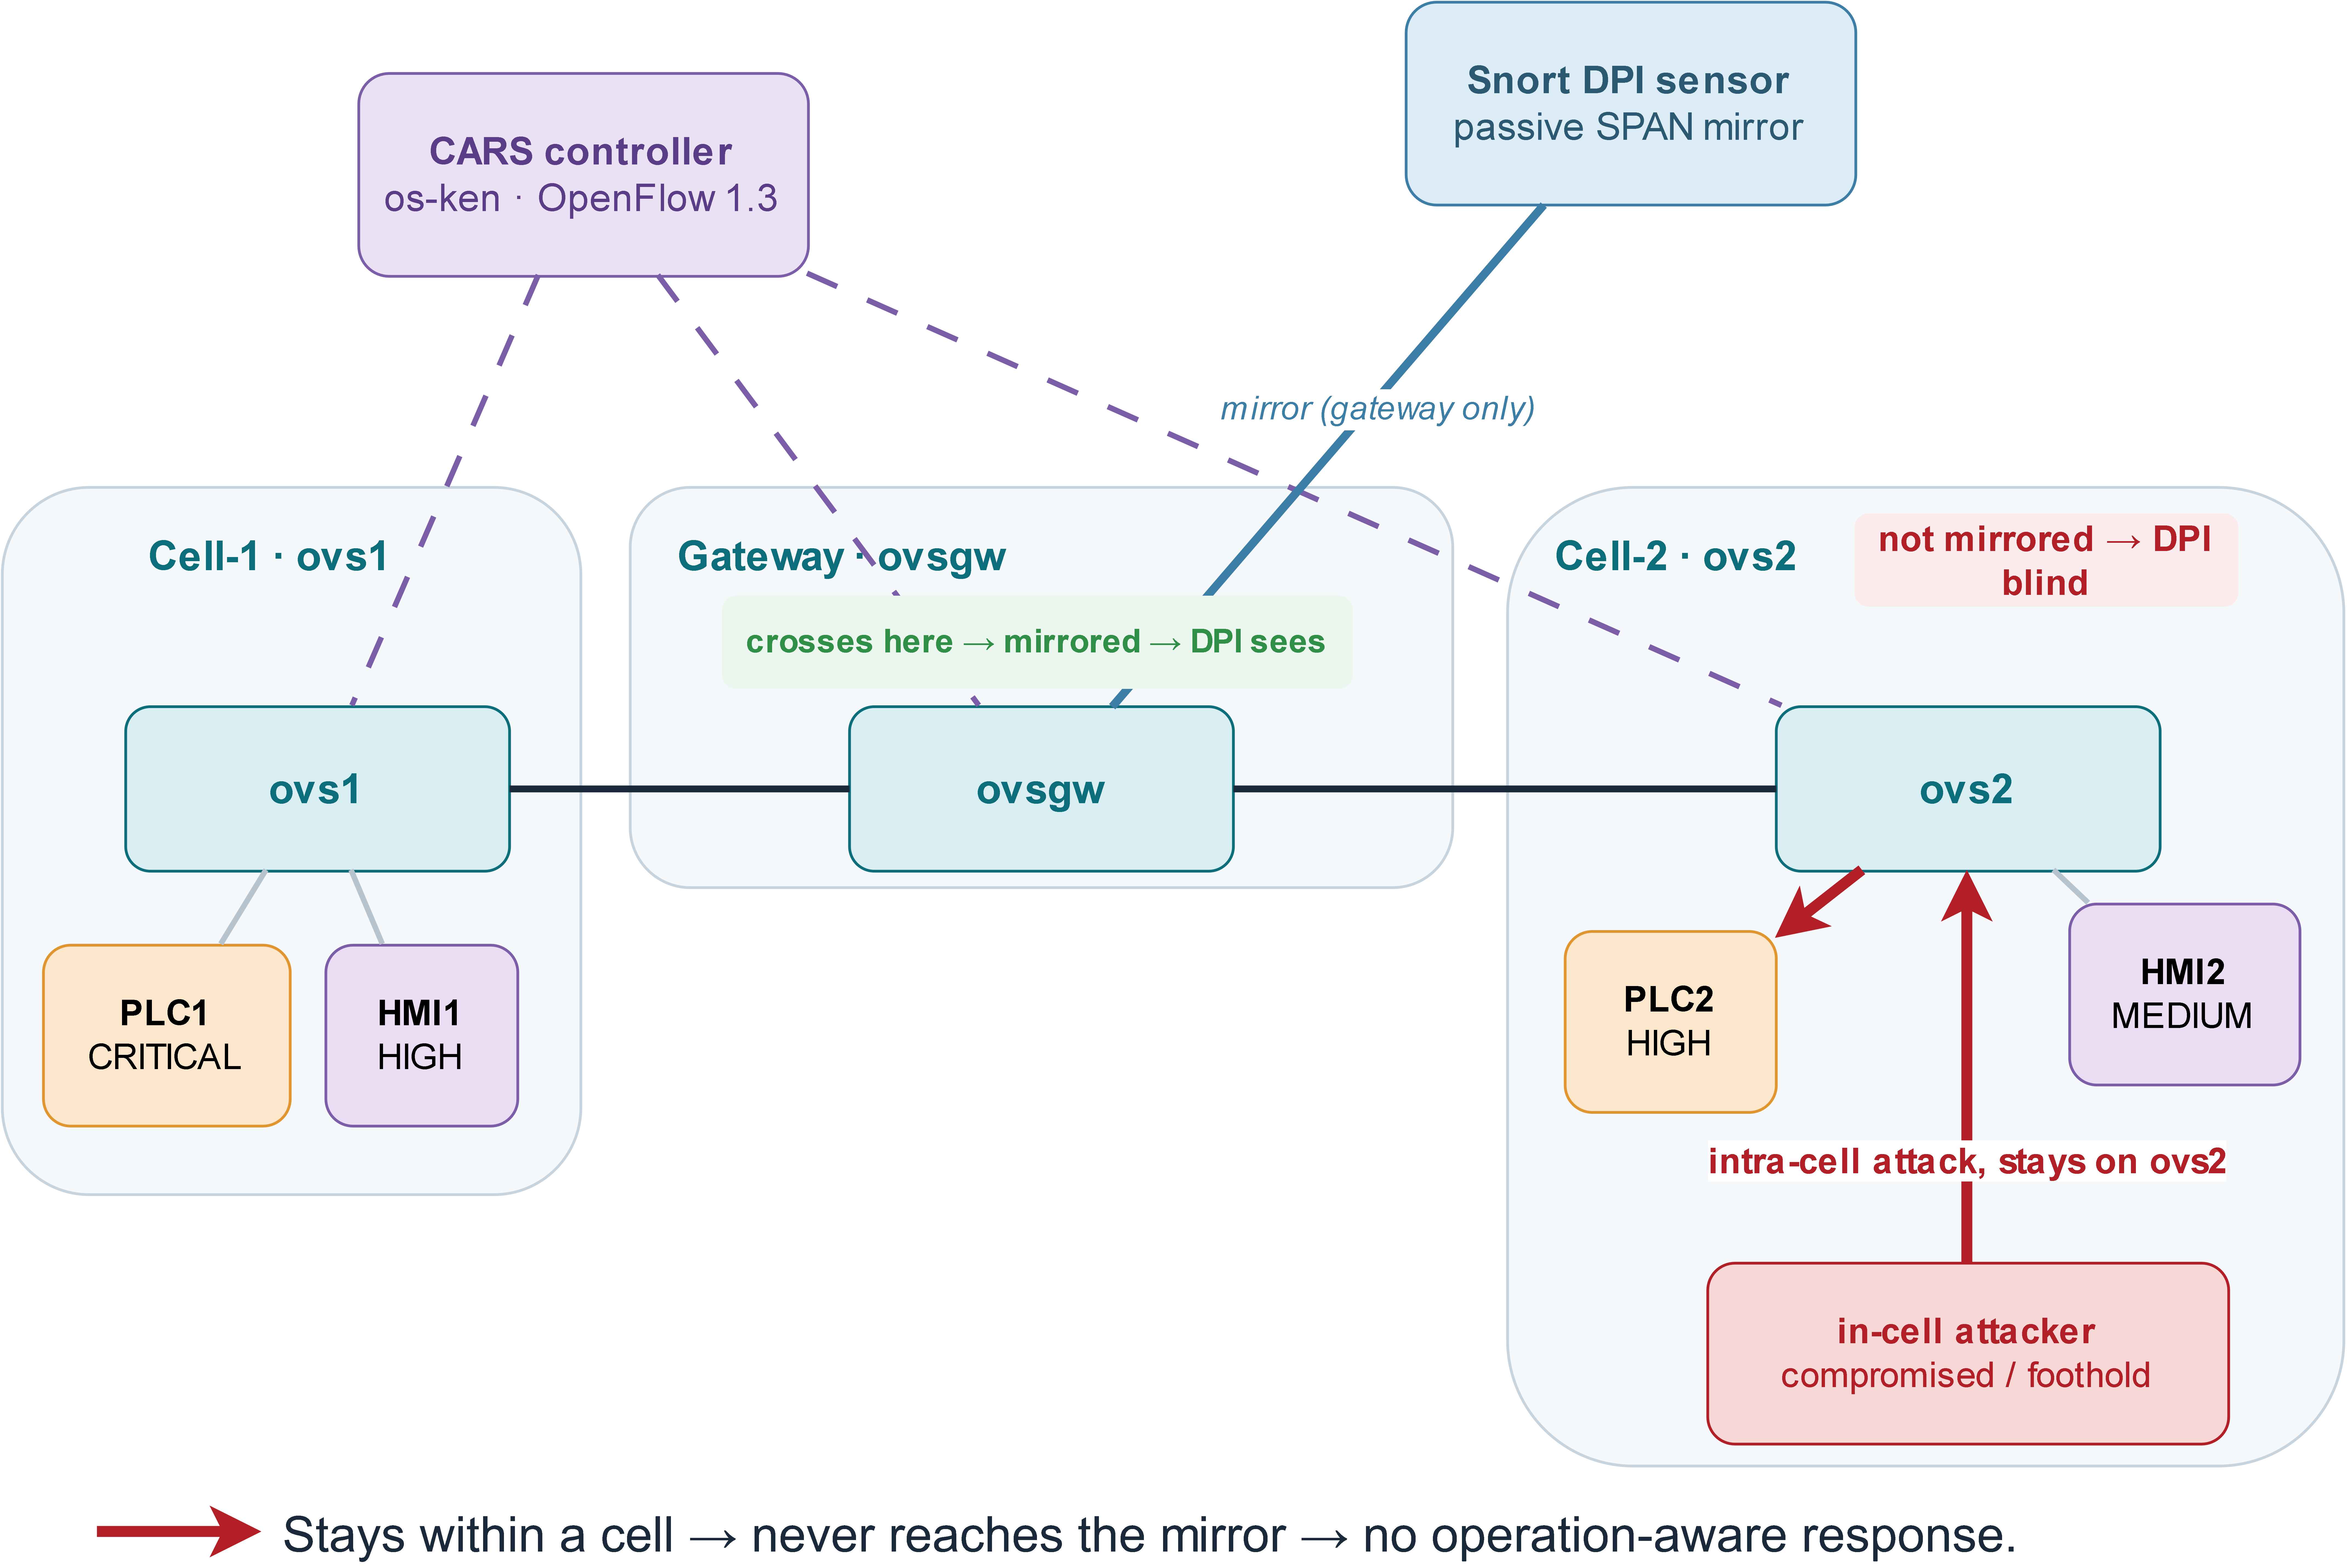
\includegraphics[width=\textwidth]{fig_cellblindspot.png}
\caption{The spatial coverage of the operation-aware tier. The Snort mirror taps \texttt{ovsgw} only: gateway-crossing traffic is inspected (green), while a purely intra-cell path (red), an in-cell foothold reaching \texttt{PLC2} over \texttt{ovs2}, never reaches the mirror and is not operation-aware. The proactive layer still applies on every switch, so an unregistered intra-cell source is refused regardless. This is an architectural illustration of a coverage boundary, not a tested attack.}
\label{fig:cellblindspot}
\end{figure}

\section{Runtime state}
\label{appx:runtime}

Two further live checks referenced from Section~\ref{sec:implementation}. Figure~\ref{fig:appguard} is the GUARD anti-spoof drop counter for every binding on every switch, all at zero under normal operation. Figure~\ref{fig:appmeter} is the rate-limiting meter that backs the THROTTLE response.

\begin{figure}[h]
\centering
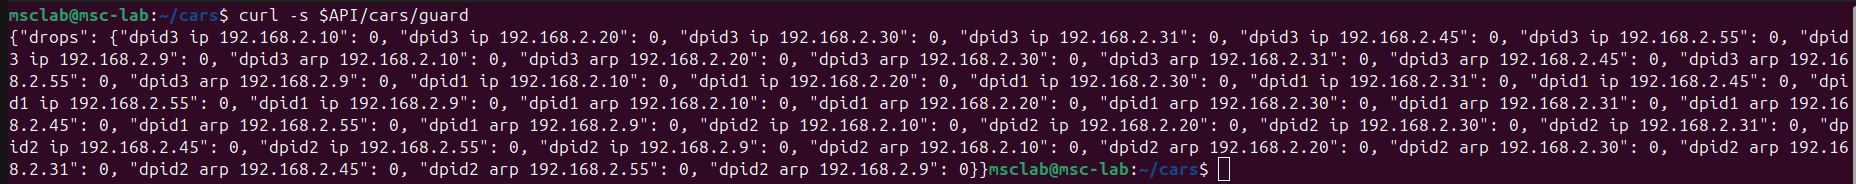
\includegraphics[width=\textwidth]{term_guard.png}
\caption{GUARD anti-spoof drop counters from \texttt{curl \$API/cars/guard}, per binding and per switch (all zero, armed and quiescent).}
\label{fig:appguard}
\end{figure}

\begin{figure}[h]
\centering
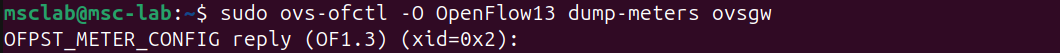
\includegraphics[width=\textwidth]{term_meter.png}
\caption{The OpenFlow meter behind the THROTTLE response, from \texttt{ovs-ofctl dump-meters ovsgw}.}
\label{fig:appmeter}
\end{figure}

\section{Complete evaluation matrix}
\label{appx:matrix}

The full decision matrix of Section~\ref{sec:evalaccuracy}, all twenty-seven cases with the columns the body table abbreviates (source, destination, operation, rate, ground-truth label, tier, response, verdict, note), regenerated from the deployed engine via \texttt{/cars/respond}.

\lstinputlisting[style=carssrc,caption={The evaluation matrix, \texttt{cars\_eval\_matrix.csv}.},label={lst:matrix}]{appendix_listings/eval_matrix.csv}

\section{Decision logs and events}
\label{appx:logs}

The controller logs every decision it takes, so the conformance result rests on thousands of live judgements, not only the scored matrix. Listing~\ref{lst:decisions} is a representative extract spanning the campaign: the reconnaissance isolate, the identity-spoof refusal, the mean-time-to-mitigate isolate, the operation-aware isolate, the flow-integrity drift, and two legitimate operations permitted. The complete per-run logs are the exported CSV artefacts (each run logs on the order of a thousand decisions).

\lstinputlisting[style=carssrc,caption={Representative controller decisions across the campaign (extract of the decision log; times \texttt{08-05}).},label={lst:decisions}]{appendix_listings/decision_extract.csv}

\section{Packet-level and wire-level analysis}
\label{appx:wire}

The wire evidence is dissected directly from the captured pcaps. On the S7 side, the attacker's Write-Var frames to PLC1 were counted at the two synchronised capture points, the Snort mirror and the PLC's physical port, armed and disarmed, giving the drop-on-the-wire result of Table~\ref{tab:wiredrop}: eight write attempts seen by the detector, one reaching the PLC when armed against seven when disarmed.

On the Modbus side, the operation-awareness discriminator is visible in the frame bytes. The same conduit \texttt{192.168.2.31 $\to$ 192.168.2.20:502} carried a read and a write, distinguished only by the function code at offset seven of the payload:

\begin{lstlisting}[style=carssrc,caption={Modbus read and write on the same conduit; the function code sits at offset 7.},label={lst:modbusfc}]
READ  (-> ALLOW)     MBAP+PDU: 00 01 00 00 00 06 00 03 00 00 00 04
                     tid=0001 proto=0000 len=0006 unit=00 FC=03  (read holding)
WRITE (-> THROTTLE)  MBAP+PDU: 00 01 00 00 00 06 00 06 00 04 00 07
                     tid=0001 proto=0000 len=0006 unit=00 FC=06  (write register)
\end{lstlisting}

\noindent CARS allowed the FC\,03 read and throttled the FC\,06 write on that single byte. The dangerous function codes (\texttt{0x05} control, \texttt{0x08} diagnostic, \texttt{0x2B} program, \texttt{0x64} illegal) and the reliability with which the sensor detects each are given in Table~\ref{tab:dpi}. Figure~\ref{fig:modbusdpi} shows the two Modbus function-code fields as Wireshark dissects them.

\begin{figure}[h]
\centering
\begin{minipage}[t]{0.49\textwidth}\centering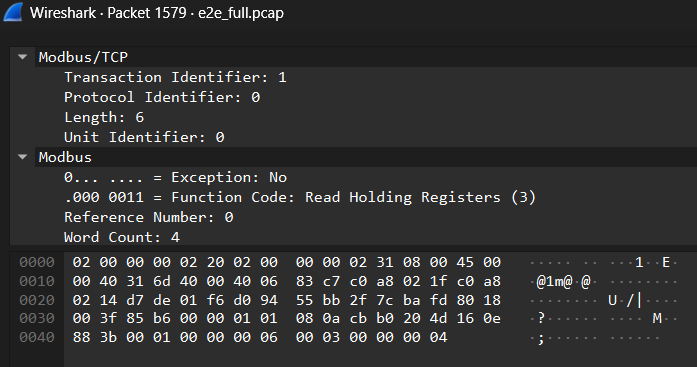
\includegraphics[width=\linewidth]{wire_modbus_fc3.png}\end{minipage}\hfill
\begin{minipage}[t]{0.49\textwidth}\centering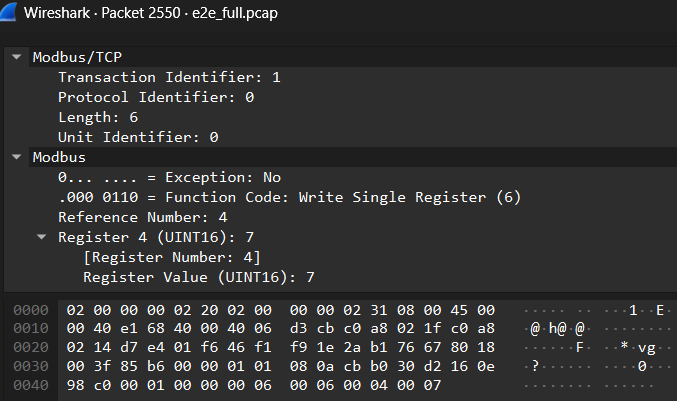
\includegraphics[width=\linewidth]{wire_modbus_fc6.png}\end{minipage}
\caption{The Modbus operation on the wire, same conduit \texttt{.31$\to$.20}. Left: \texttt{Function Code: Read Holding Registers (3)}, permitted. Right: \texttt{Function Code: Write Single Register (6)} setting register~4 to~7, throttled. The verdict turns on this field.}
\label{fig:modbusdpi}
\end{figure}

Two further S7 views complete the picture. Figure~\ref{fig:wiredisarmed} shows the attacker's write reaching the PLC with CARS disarmed (contrast the single armed write of Figure~\ref{fig:wireproof}). Figure~\ref{fig:s7stream} shows that lone attacker frame amongst the legitimate Factory IO loop traffic on the PLC port, the attack is a needle in the live process stream.

\begin{figure}[h]
\centering
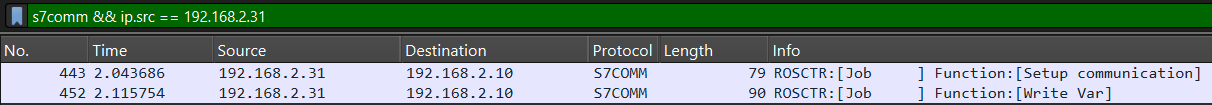
\includegraphics[width=0.9\textwidth]{wire_disarmed.png}
\caption{Disarmed, the attacker's S7 Write Var (frame 452) reaches the PLC. With CARS armed the same write is dropped in the fabric (Figure~\ref{fig:wireproof}).}
\label{fig:wiredisarmed}
\end{figure}

\begin{figure}[h]
\centering
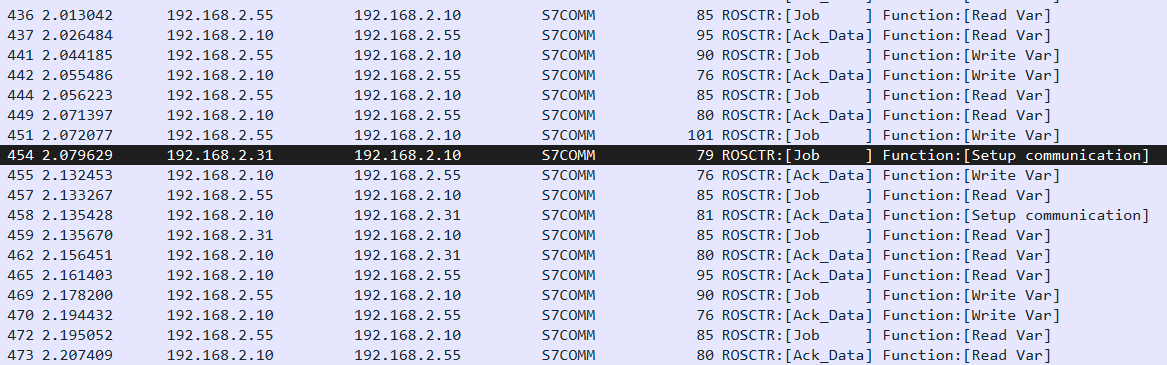
\includegraphics[width=\textwidth]{wire_s7_stream.png}
\caption{The attacker's Setup frame (\texttt{.31$\to$.10}, highlighted) amongst the legitimate \texttt{.55} Factory IO loop traffic on the PLC port. CARS must pick the malicious operation out of a continuous stream of legitimate S7 reads and writes.}
\label{fig:s7stream}
\end{figure}

The enforcement itself is visible on a third wire, the OpenFlow control channel (TCP~6653), captured in \texttt{of\_control.pcap}. Listing~\ref{lst:flowmod} is the \texttt{OFPT\_FLOW\_MOD} that installs the reactive isolate, decoded from that capture: an ADD of the drop rule stamped with the CARS reactive cookie \texttt{0x00ca}, at priority~110 in the POLICY table, matching the attacker's source with a 75-second self-healing timeout. Two identical messages are sent, one to \texttt{ovs1} and one to \texttt{ovsgw}, so the quarantine is installed fabric-wide from a single decision. This is the control-plane counterpart to the datapath dump of Figure~\ref{fig:p6armedflow}: the rule seen being installed, not just seen in place.

\begin{lstlisting}[style=carssrc,caption={The reactive isolate as an \texttt{OFPT\_FLOW\_MOD}, decoded from \texttt{of\_control.pcap} (OpenFlow 1.3, tcp/6653).},label={lst:flowmod}]
OFPT_FLOW_MOD              (version 0x04, type 14, control channel tcp/6653)
  command      = ADD
  cookie       = 0x00000000000000ca     (CARS reactive marker; 0xa2 = static A2 policy)
  table_id     = 1                        (POLICY)
  priority     = 110                       (above the allowlist and default-deny)
  hard_timeout = 75 s                      (CRITICAL asset: 30 + 15*3, then self-heals)
  match        = eth_type=0x0800, ipv4_src=192.168.2.31
  instructions = APPLY_ACTIONS []          (no output action = drop)
-> sent to ovs1 and ovsgw from one controller decision (fabric-wide quarantine)
\end{lstlisting}

\section{Scenario testing in full}
\label{appx:scenarios}

The process devastation of Section~\ref{sec:evaldevastation} has a second, quieter variant: instead of driving the tank visibly over the top, the attacker pins the reported level near zero, so the operator panel shows a safe, empty tank while the real one fills. Figure~\ref{fig:p6deception} captures this deception from a disarmed run: the real Factory IO tank stands filled while the HMI reads a level of zero and a pump of \texttt{+0.000}.

\begin{figure}[h]
\centering
\begin{minipage}[c]{0.42\textwidth}\centering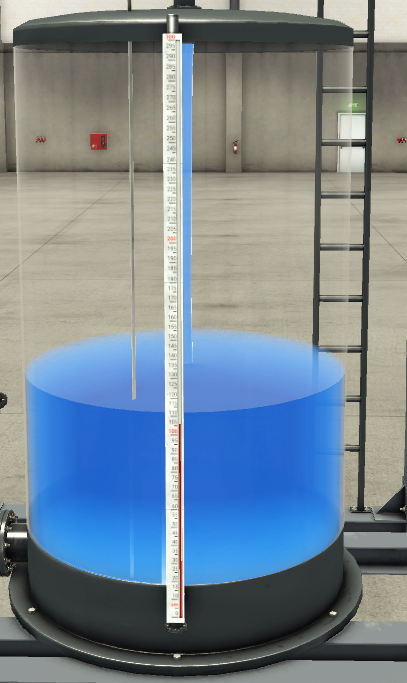
\includegraphics[width=\linewidth]{p6_tank_disarmed.png}\end{minipage}\hfill
\begin{minipage}[c]{0.54\textwidth}\centering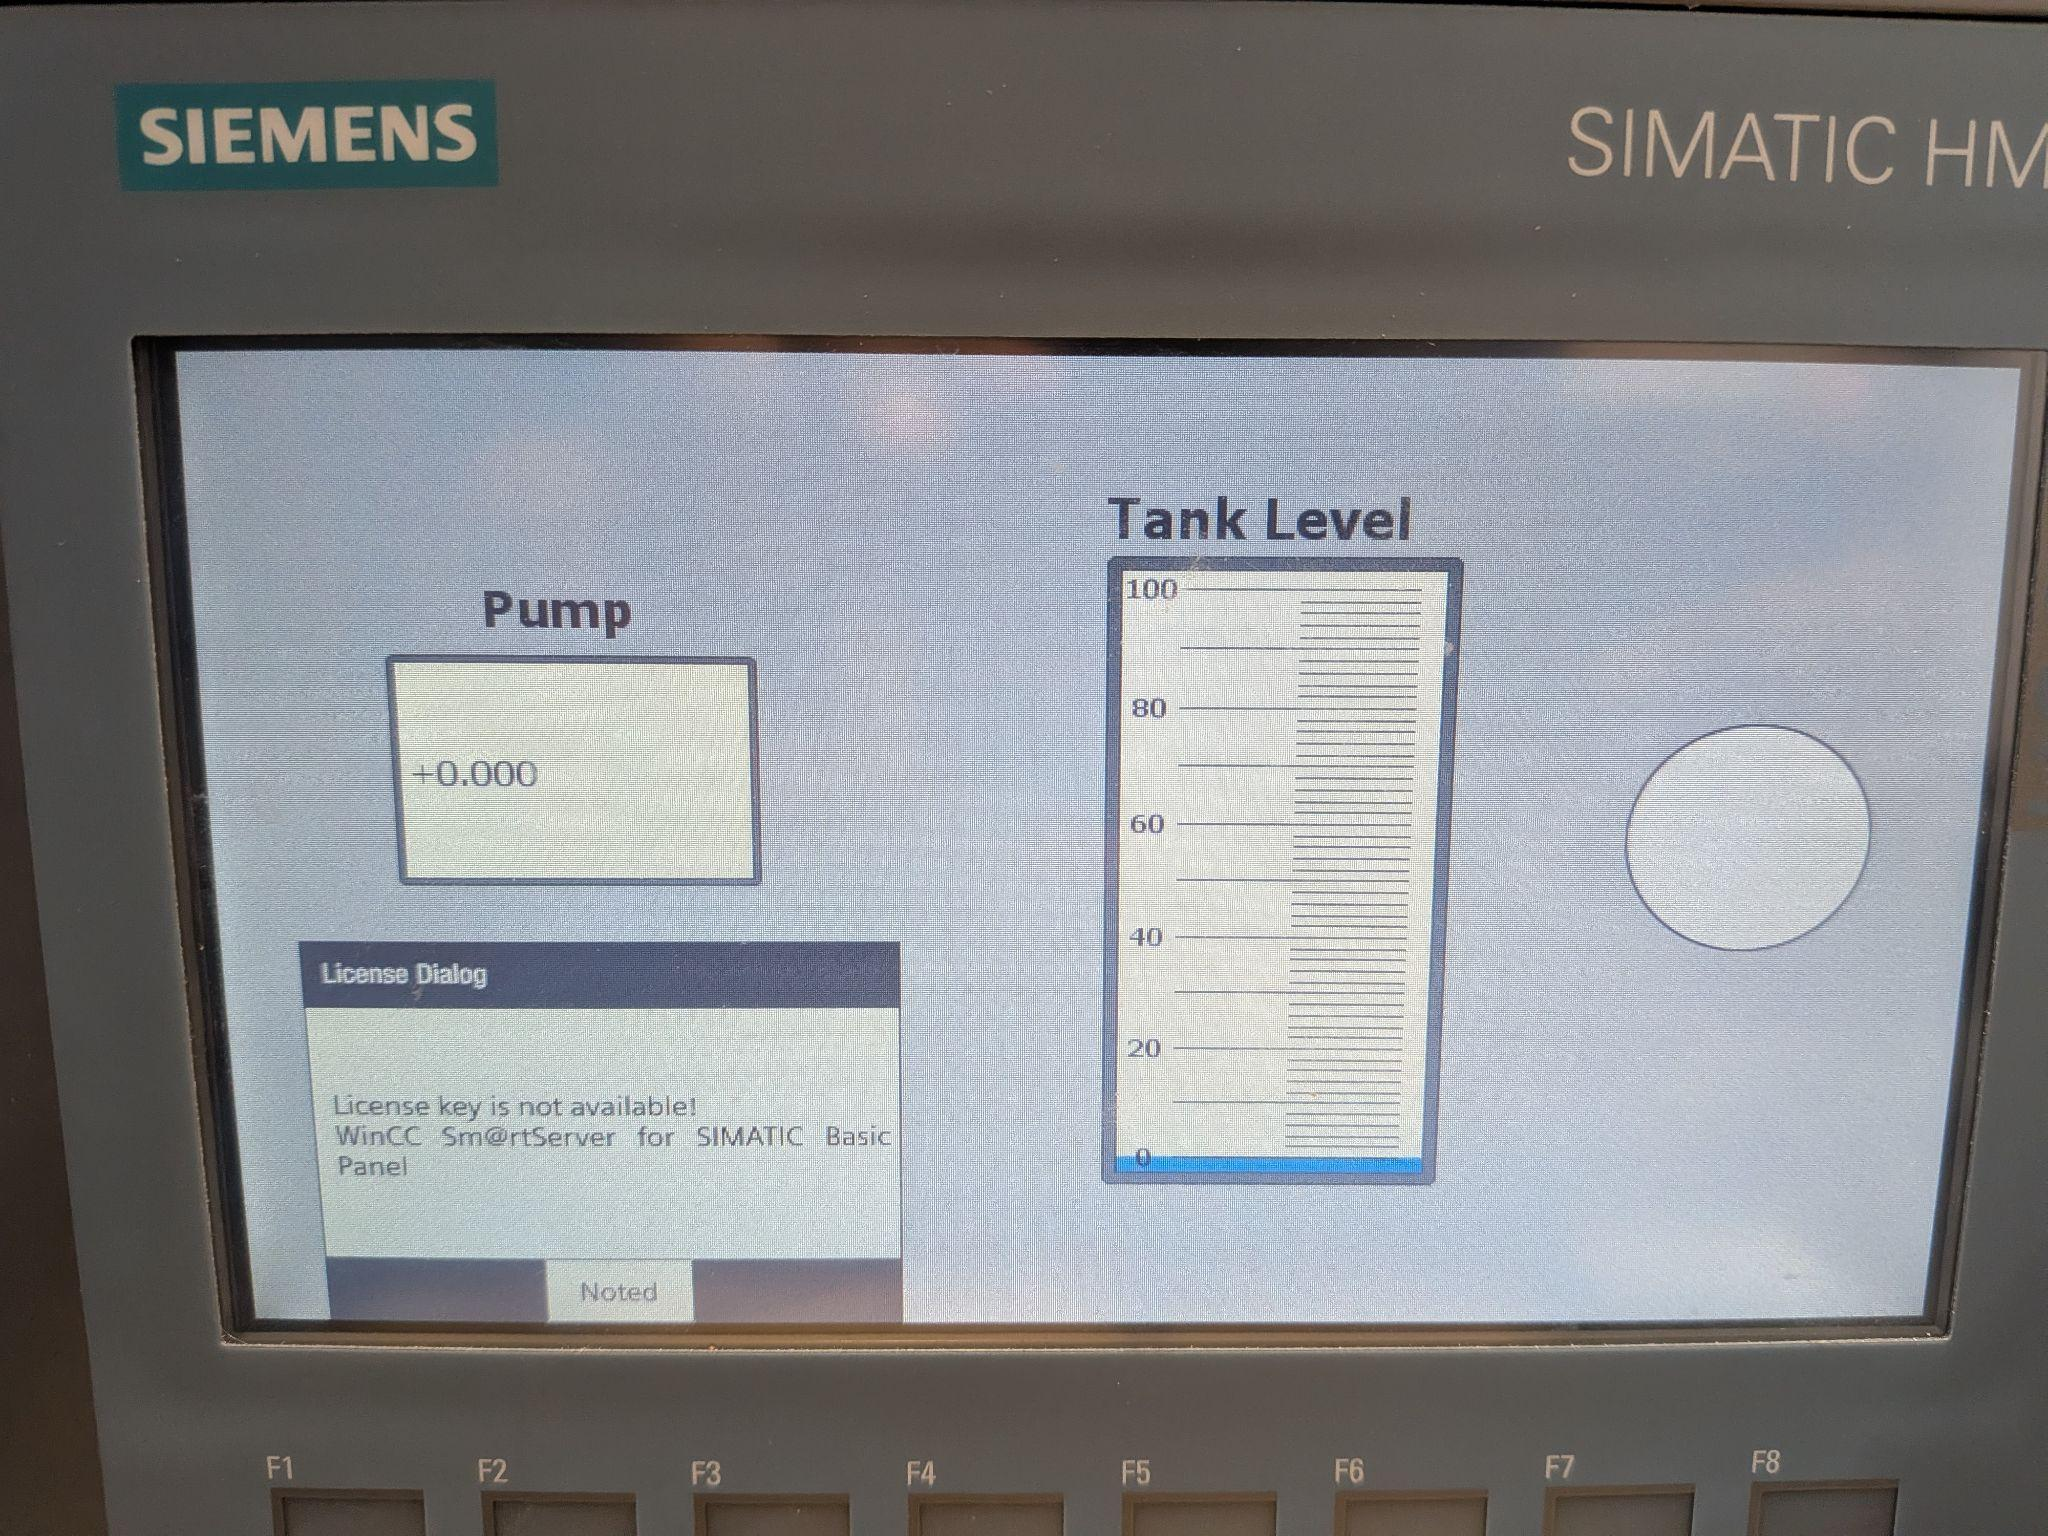
\includegraphics[width=\linewidth]{p6_hmi_deceived.jpg}\end{minipage}
\caption{The sensor-spoof deception, disarmed. Left: the real Factory IO tank, filled. Right: the operator HMI at the same moment, reading zero. The reported process has been divorced from the real one.}
\label{fig:p6deception}
\end{figure}

The external vectors were driven from the Kali attacker \texttt{192.168.2.77}. Reconnaissance under CARS is shown in Figure~\ref{fig:p1recon}: an armed port scan of the PLC returns every port \texttt{filtered}, and the scan is reactively isolated with a criticality-scaled quarantine. Identity spoofing is shown in Figure~\ref{fig:p2spoof}: the GUARD anti-spoof drop counters register the forged ARP frames dropped at ingress. The reaction window over one hundred autonomous trials is in Figure~\ref{fig:mttm}.

\begin{figure}[h]
\centering
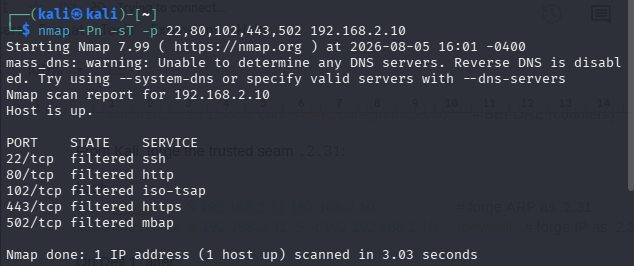
\includegraphics[width=0.82\textwidth]{p1_recon_ports.png}\\[4pt]
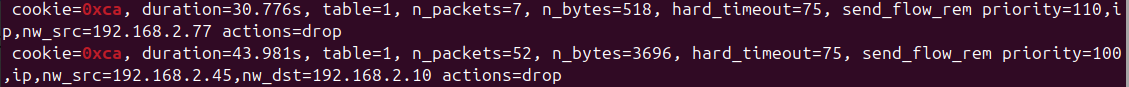
\includegraphics[width=0.82\textwidth]{p1_recon_isolate.png}
\caption{Reconnaissance from Kali, armed. Top: the port scan of PLC1, every port \texttt{filtered}. Bottom: the reactive rule installed against the scanner, \texttt{cookie=0xca}, \texttt{priority=110}, \texttt{nw\_src=192.168.2.77}, \texttt{actions=drop}, \texttt{hard\_timeout=75}.}
\label{fig:p1recon}
\end{figure}

\begin{figure}[h]
\centering
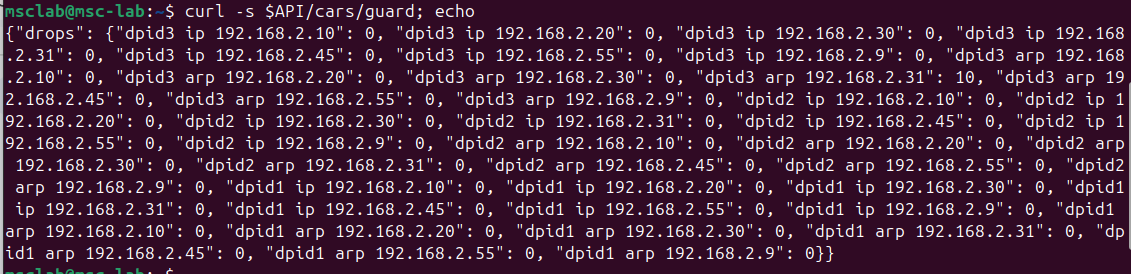
\includegraphics[width=\textwidth]{p2_guard_after.png}
\caption{Identity spoofing at GUARD. After forging ARP as the trusted seam \texttt{192.168.2.31} from Kali, the anti-spoof counter \texttt{dpid3 arp 192.168.2.31} registers the dropped frames (running total 10), every forged frame dropped at ingress with all other bindings untouched. The controller logged each as \texttt{REFUSED (identity-spoof)}.}
\label{fig:p2spoof}
\end{figure}

\begin{figure}[h]
\centering
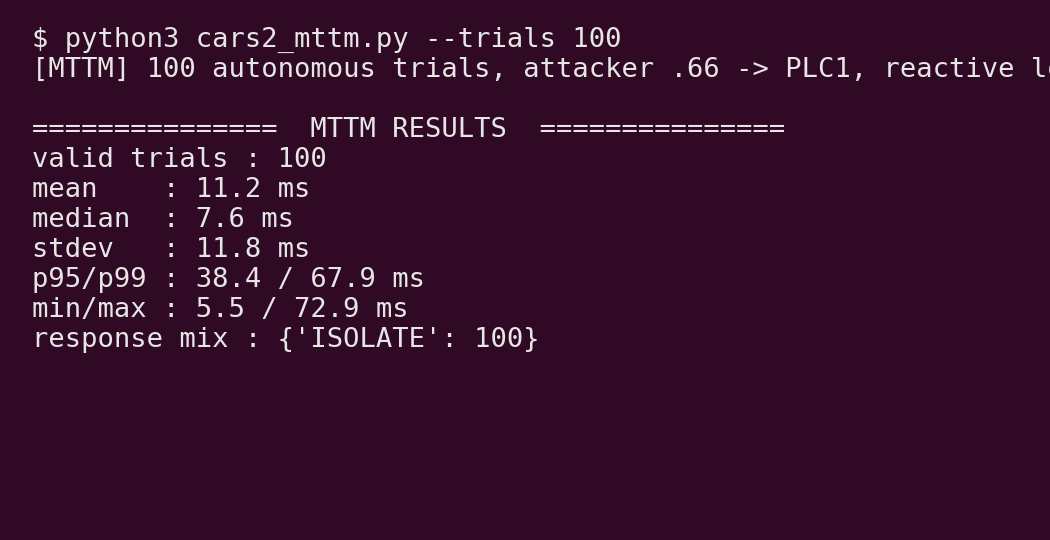
\includegraphics[width=0.9\textwidth]{p2_mttm.png}
\caption{Reaction window (mean-time-to-mitigate) over one hundred autonomous trials, attack-frame to enforcement on a single clock: median 7.6\,ms, mean 11.2\,ms, standard deviation 11.8\,ms, minimum 5.5\,ms, maximum 72.9\,ms, every trial ending in ISOLATE.}
\label{fig:mttm}
\end{figure}

\section{Scripts and code}
\label{appx:code}

Each script is presented as its role plus its load-bearing snippet. The lead is the controller, \href{\repourl/blob/main/06_Build/cars_engine.py}{\texttt{cars\_engine.py}}: the whole evaluation drives its decision path, whose core is \texttt{classify()}, mapping a (source, destination, operation) to a tier by walking the rulebook first-match-wins.

\begin{lstlisting}[style=carssrc,caption={The controller decision path (\href{\repourl/blob/main/06_Build/cars_engine.py}{\texttt{cars\_engine.py}}): first-match rulebook classification.},label={lst:classify}]
def classify(src_ip, dst_ip, op=None):
    s, d = role_of(src_ip), role_of(dst_ip)      # map IP -> role from the REGISTRY
    for rsrc, rdst, rop, tier in RULEBOOK:        # rules in priority order
        if (rsrc == "any" or rsrc == s or rsrc == src_ip) and \
           (rdst == "any" or rdst == d or rdst == dst_ip) and \
           (rop  == "any" or rop  == op):
            return tier, s, d                     # first match wins -> its tier
    return "FORBIDDEN", s, d                       # nothing matched -> default deny
\end{lstlisting}

\noindent The role lookup resolves each address to its registered role; the loop returns the tier of the first rulebook row whose source, destination and operation all match, and defaults to FORBIDDEN when none do. This is the exact path the conformance evaluation drives through \texttt{/cars/respond}. The remaining load-bearing pieces of the controller and of the supporting scripts follow in the same form.

\subsection*{Controller: the rest of the decision-to-enforcement path}

\noindent \textbf{Criticality elevation and block duration (\texttt{respond()}).} After classification, the destination's criticality weight drives two things: a trusted actuating write (SENSITIVE) to a CRITICAL asset is elevated to FORBIDDEN unless an authorised maintenance window is open, and the quarantine duration is scaled by the same weight.

\begin{lstlisting}[style=carssrc,caption={Grey-zone elevation and criticality-scaled block duration.},label={lst:elevate}]
acl = crit_of(dst_ip); dcw = CW.get(acl, 0)          # dst asset weight: 3..0
in_window = time.time() < self.maint_until
elevated = (tier == "SENSITIVE" and dcw >= 3 and not in_window)
if elevated:
    tier = "FORBIDDEN"          # trusted WRITE to a CRITICAL asset -> forbidden
timeout = BLOCK_TIMEOUT + dcw * 15   # CRITICAL 75, HIGH 60, MED 45, LOW 30 s
\end{lstlisting}

\noindent \textbf{The graded response ladder (\texttt{select\_response()}).} A tier, the asset weight and a rate flag select one of the seven responses; the safety loop is never enforced against, and higher-criticality assets escalate sooner and skip rungs.

\begin{lstlisting}[style=carssrc,caption={Criticality-graded, flood-aware response selection.},label={lst:selresp}]
if tier == "CRITICAL":    return "REFUSE"        # safety invariant - never enforce
esc = max(1, ESCALATE - dcw); c = state.get("count", 1)
if tier == "OPERATIONAL":
    if flood:
        if dcw >= 3: return "BLOCK"              # flood on CRITICAL asset -> cut
        return "THROTTLE" if c < esc else "BLOCK"
    return "ALLOW"                                # trusted conduit, normal rate
if tier == "SENSITIVE":
    if flood:    return "BLOCK"
    if dcw >= 3: return "BLOCK"                   # CRITICAL asset: skip THROTTLE
    return "THROTTLE" if c < esc else "BLOCK"
if flood:    return "ISOLATE"                     # FORBIDDEN
if dcw >= 3: return "ISOLATE"                     # CRITICAL asset: isolate now
return "BLOCK" if src_count < esc else "ISOLATE"
\end{lstlisting}

\noindent \textbf{The reactive install (\texttt{isolate\_source()}).} Every enforcement is a real OpenFlow rule stamped with the distinct reactive cookie \texttt{0x00ca}, self-expiring via \texttt{hard\_timeout} and notifying the controller on removal (\texttt{SEND\_FLOW\_REM}) so the defence self-heals when the attack stops. Isolation drops all traffic from the source across every switch.

\begin{lstlisting}[style=carssrc,caption={Source quarantine: a self-healing drop on every switch (\texttt{REACTIVE\_COOKIE = 0x00CA}).},label={lst:isolate}]
def isolate_source(self, src_ip, timeout=BLOCK_TIMEOUT):
    for d, dp in list(self.datapaths.items()):
        ofp, psr = dp.ofproto, dp.ofproto_parser
        m = psr.OFPMatch(eth_type=0x0800, ipv4_src=src_ip)      # any dst
        dp.send_msg(psr.OFPFlowMod(datapath=dp, cookie=REACTIVE_COOKIE,
            table_id=1, priority=110, match=m, instructions=[],  # [] = drop
            hard_timeout=timeout, flags=ofp.OFPFF_SEND_FLOW_REM))
\end{lstlisting}

\noindent \textbf{Anti-spoof GUARD (\texttt{install\_guard()}).} Table~0 binds each protected identity to its physical port and MAC; a frame carrying a protected source address that does not arrive on its bound port is dropped before it can reach policy. This is prevention, not detection.

\begin{lstlisting}[style=carssrc,caption={Table 0 identity binding and anti-spoof drop.},label={lst:guard}]
for (d, port, mac, ip) in BINDINGS:                # bind identity to port+MAC
    if d == dp.id:
        add(200, OFPMatch(in_port=port, eth_type=0x0800,
                          eth_src=mac, ipv4_src=ip), GOTO)   # legit -> policy
if GUARD_ENABLED:
    for ip in PROTECTED_IPS:
        add(100, OFPMatch(eth_type=0x0800, ipv4_src=ip), [])  # forged src -> drop
add(0, OFPMatch(), GOTO)                            # default -> policy table
\end{lstlisting}

\noindent \textbf{Control-API authentication (\texttt{\_app()}).} Every state-changing endpoint requires a shared token; the read-only status endpoints and the Snort detection feed are excluded so the bridge is unchanged.

\begin{lstlisting}[style=carssrc,caption={Token gate on the control endpoints.},label={lst:auth}]
_CONTROL = ('/cars/defense','/cars/maintenance','/cars/reload','/cars/reload-a2',
            '/cars/block','/cars/unblock','/cars/restore')
if path in _CONTROL and environ.get('HTTP_X_CARS_TOKEN','') != self.api_token:
    return reply({"error": "unauthorized - X-CARS-Token required"}, '401 Unauthorized')
# /cars/respond (Snort bridge feed) is intentionally excluded
\end{lstlisting}

\subsection*{The supporting scripts}

\noindent \textbf{Detection bridge (\href{\repourl/blob/main/06_Build/snort_bridge.py}{\texttt{snort\_bridge.py}}).} Snort raises the alerts; the bridge recovers the ICS operation from the alert text, measures its arrival rate, and posts the source, destination, operation and rate to the controller, which alone decides. The brain, not the sensor, holds the policy.

\begin{lstlisting}[style=carssrc,caption={Operation recovery from the Snort alert, forwarded to the controller.},label={lst:bridge}]
API = "http://10.10.10.1:8080/cars/respond"     # the brain decides; bridge only reports
mo = re.search(r'CARS-(MODBUS|S7)-(WRITE|READ|CONTROL|DIAG|PROGRAM|ILLEGAL)', line)
if mo: proto = mo.group(1); op = mo.group(2)     # recover the operation
key = (src, dst, op)                             # keep read vs write distinct
# rate of this (src,dst,op) measured, then POSTed with op+rate to API
\end{lstlisting}

\noindent \textbf{Flow-integrity self-check (\href{\repourl/blob/main/06_Build/cars_flow_audit.py}{\texttt{cars\_flow\_audit.py}}).} A trusted baseline of the immutable policy (Table~0 GUARD and the Table~1 A2 allowlist, cookie \texttt{0xa2}) is captured at a clean start; the only additions permitted at runtime are the reactive rules (cookie \texttt{0xca}). Anything else appearing on a switch is flagged as drift and surfaced into the controller's decision log.

\begin{lstlisting}[style=carssrc,caption={Flow identity and the drift model.},label={lst:flowaudit}]
# identity = bridge,table,priority,cookie,MATCH (not actions): a tampered action on a
# policy rule shows as "changed"; a bogus new rule as "extra".
def key_of(br, s): return "%s|t%s|p%s|c%s|%s" % (br, s[0], s[1], s[2], s[3])
# baseline = GUARD (t0) + A2 allowlist (t1, cookie 0xa2); the ONLY legitimate live
# additions carry the reactive cookie 0xca. Anything else later -> drift -> audit.
\end{lstlisting}

\noindent \textbf{Process-state remediation (\href{\repourl/blob/main/06_Build/cars_remediation.py}{\texttt{cars\_remediation.py}}).} The novel maintain half of block-and-maintain: it detects sensor tampering by process anomaly (a level the bang-bang control law physically cannot produce) and writes the last-good value back over S7, holding the process while the source is quarantined.

\begin{lstlisting}[style=carssrc,caption={Anomaly-triggered last-good restore over S7.},label={lst:remediation}]
last_good = SEED
while True:
    lvl = s7_read(c)                         # read Tank.Level over S7
    if tampered(lvl, prev):                  # a value the control law cannot produce
        s7_write(c, last_good)               # RESTORE last-good on tamper
        feed("RESTORED", level=round(lvl,1), last_good=round(last_good,1))
    else:
        last_good = lvl                       # healthy -> advance last-good
\end{lstlisting}

\noindent \textbf{Latency harness (\href{\repourl/blob/main/07_Evaluation/cars2_mttm.py}{\texttt{cars2\_mttm.py}}).} Times the reaction window on a single clock: start the attack, poll for the isolate to appear in the controller's block set, and record attack-frame-to-enforcement.

\begin{lstlisting}[style=carssrc,caption={Single-clock mean-time-to-mitigate measurement.},label={lst:mttm}]
t0 = time.time()
# ... launch the attack ...
while not blocked() and time.time() - t0 < 15: time.sleep(0.02)  # poll for isolate
mttm = time.time() - t0                       # attack-frame -> enforcement
\end{lstlisting}

\noindent \textbf{Attack tool (\href{\repourl/blob/main/06_Build/cars_fdi_overflow.py}{\texttt{cars\_fdi\_overflow.py}}).} The false-data injection used in Section~\ref{sec:evalcampaign}: a compromised host opens an S7 session to the PLC and writes the output area at high rate, blinding the level sensor and jamming the discharge valve. Each write is a CONTROL operation to the output area, which CARS recovers and forbids.

\begin{lstlisting}[style=carssrc,caption={The FDI overflow injection (writes to the S7 output area).},label={lst:fdi}]
c = snap7.client.Client(); c.connect(HOST, 0, 1)   # HOST = PLC 192.168.2.10
zero = bytearray(struct.pack('>f', 0.0))
while time.time() < end:
    c.write_area(PE, 0, 100, zero)   # blind LevelIn %ID100 = 0 (sensor OB30 trusts)
    c.write_area(PA, 0, 104, zero)   # jam DischargeValve %QD104 = 0 (output area 0x82)
\end{lstlisting}

\subsection*{Evaluation and proof harnesses}

\noindent \textbf{Conformance harness (\href{\repourl/blob/main/06_Build/cars_eval.py}{\texttt{cars\_eval.py}}).} Drives the labelled case set of Section~\ref{sec:evalaccuracy} through the deployed engine over \texttt{/cars/respond}, scores each answer against its intent label, and writes \texttt{cars\_eval\_matrix.csv}. It disarms for the decision-only pass so nothing is enforced on the live conduits, then re-arms.

\begin{lstlisting}[style=carssrc,caption={Driving each case through the engine and scoring it against intent.},label={lst:eval}]
def respond(src,dst,op,rate=0,dpid=1):            # one case -> the deployed decision path
    return post("/cars/respond",{"src":src,"dst":dst,"op":op,"proto":"S7","dpid":dpid,"rate":rate})
def verdict(label,resp):
    permit = resp in {"ALLOW","MONITOR","REFUSE"}
    if label in ("legit","flood_exempt"): return "TN" if permit else "FP"
    if label == "attack":                 return "TP" if not permit else "FN"
    return "grey"                                 # grey rows shown, not scored
post("/cars/defense",{"on":False},auth=True)      # decision-only pass; re-armed at the end
\end{lstlisting}

\noindent \textbf{Criticality sweep (\href{\repourl/blob/main/06_Build/cars_criticality_proof.sh}{\texttt{cars\_criticality\_proof.sh}}).} Holds the actor and operation fixed and varies only the target's tier. Part~1 runs disarmed to show the bounded elevation as a pure decision; Part~2 runs armed to measure the tier-scaled quarantine ($30 + 15w$ seconds), healing the reactive rule after each fire.

\begin{lstlisting}[style=carssrc,caption={Fire a controlled case, and heal the tier-scaled reactive rule between fires.},label={lst:critproof}]
fire(){ curl -s -XPOST $API/respond -H 'Content-Type: application/json' \
        -d "{\"src\":\"$2\",\"dst\":\"$3\",\"proto\":\"$4\",\"op\":\"$5\",\"dpid\":3}"; }
heal(){ for sw in ovsgw ovs1; do sudo ovs-ofctl -O OpenFlow13 --strict del-flows "$sw" "table=1,priority=110"; done; }
arm false     # PART 1 - decision side: bounded elevation, nothing enforced
arm true      # PART 2 - response side: real quarantine, hard_timeout = 30 + cw*15 s
\end{lstlisting}

\noindent \textbf{Campaign library (\href{\repourl/blob/main/06_Build/cars_campaign_lib.sh}{\texttt{cars\_campaign\_lib.sh}}).} The shared helpers every campaign and pivot run sources: arm/disarm through the authenticated API, a cross-layer \texttt{snap} of the live state, and \texttt{capstart} which opens the three synchronised wire captures.

\begin{lstlisting}[style=carssrc,caption={Arm/disarm and the three-point capture used across the campaign.},label={lst:camplib}]
arm(){    curl -s -X POST $API/cars/defense -H "X-CARS-Token: $TOKEN" -d '{"on":true}';  }
disarm(){ curl -s -X POST $API/cars/defense -H "X-CARS-Token: $TOKEN" -d '{"on":false}'; }
capstart(){ sudo tcpdump -i "$PLCIF" -w "$d/plc1_wire.pcap" $filt &     # what reaches the PLC
            sudo tcpdump -i any     -w "$d/of_control.pcap" 'tcp port 6653' &  # the OpenFlow flow_mods
            sudo tcpdump -i snort0  -w "$d/dpi_mirror.pcap" & }          # what the detector sees
\end{lstlisting}

\noindent \textbf{Wire campaign (\href{\repourl/blob/main/06_Build/cars_wire_campaign.sh}{\texttt{cars\_wire\_campaign.sh}}, \href{\repourl/blob/main/06_Build/cars_wire_campaign_disarmed.sh}{\texttt{cars\_wire\_campaign\_disarmed.sh}}).} Runs each attack vector against the armed system (and its disarmed twin), capturing the three wire points and timestamp-aligned state from every layer. The first vector is the control-plane disarm attempt.

\begin{lstlisting}[style=carssrc,caption={The three capture points and the control-plane vector.},label={lst:wirecamp}]
sudo timeout 240 tcpdump -i "$PLCIF" -w "$D/plc1_wire.pcap" 'host 192.168.2.10 and tcp port 102' &
sudo timeout 240 tcpdump -i any     -w "$D/of_control.pcap" 'tcp port 6653' &
sudo timeout 240 tcpdump -i snort0  -w "$D/dpi_mirror.pcap" &
# V1 CONTROL-PLANE: unauth POST /cars/defense {on:false}  -> expect HTTP 401 + DENIED audit
\end{lstlisting}

\noindent \textbf{Deep end-to-end trial (\href{\repourl/blob/main/06_Build/cars_e2e.sh}{\texttt{cars\_e2e.sh}}).} Drives the full response spectrum through the real autonomous chain and records, per scenario, the four independent proofs behind Table~\ref{tab:crosslayer}: the frame on the mirror, the Snort alert, the controller decision, and the datapath enforcement.

\begin{lstlisting}[style=carssrc,caption={The four independent ground-truth layers per scenario.},label={lst:e2e}]
wirecount(){ tshark -r "$OUT/pcap/e2e_full.pcap" -Y "$1" | wc -l; }        # WIRE   : frames on the mirror
pkts(){ ovs-ofctl -O OpenFlow13 dump-flows "$1" table=1 | grep -m1 "$2" \
        | grep -oP 'n_packets=\K[0-9]+'; }                                  # OVS    : enforcement counter moved
# SNORT : delta on /var/log/snort/alert ;  CARS : tier+response in /cars/audit
\end{lstlisting}

\noindent \textbf{Packet-drop proof (\href{\repourl/blob/main/06_Build/cars_packet_proof.sh}{\texttt{cars\_packet\_proof.sh}}).} Captures the attacker's S7 frames at two synchronised points, the Snort mirror and the PLC's physical port, armed then disarmed, giving the drop-on-the-wire counts of Table~\ref{tab:wiredrop}.

\begin{lstlisting}[style=carssrc,caption={Two synchronised capture points: what the detector sees versus what reaches the PLC.},label={lst:pktproof}]
capture(){   # tag seconds
  sudo timeout "$2" tcpdump -i snort0          "host $PLC1 and tcp port 102" -w "$D/$1_mirror.pcap" &  # DPI sees
  sudo timeout "$2" tcpdump -i enx9c69d331d874 "host $PLC1 and tcp port 102" -w "$D/$1_plc1.pcap"  & } # reaches PLC
arm true; heal; capture armed 15      # then: arm false; capture disarmed 15
\end{lstlisting}

\noindent \textbf{ICS operation battery (\href{\repourl/blob/main/06_Build/cars_ics_battery.sh}{\texttt{cars\_ics\_battery.sh}}).} Fires the full ICS operation spectrum from one trusted operator (\texttt{.31}) at the Modbus unit (\texttt{.20}) and shows the three verdicts the one conduit draws, backing Table~\ref{tab:dpi}.

\begin{lstlisting}[style=carssrc,caption={Fire each operation on the same conduit and await the new decision.},label={lst:battery}]
probe(){ restore; b=$(alast); ip netns exec opns "$@" >/dev/null 2>&1; wait_dec "$b"; }
# READ -> OPERATIONAL/ALLOW | WRITE -> SENSITIVE/THROTTLE | CONTROL,DIAG,PROGRAM,ILLEGAL -> FORBIDDEN/BLOCK
\end{lstlisting}

\subsection*{Attack clients and the process model}

\noindent \textbf{S7 attack client (\href{\repourl/blob/main/06_Build/s7_write.py}{\texttt{s7\_write.py}}).} The S7 tool used across the evaluation. Its output-area write is an actuation CARS classifies as CONTROL; the \texttt{-{}-dbspoof} mode pins a false level (the sensor-spoof deception), and further modes cover monitoring, volumetric read floods and a PLC stop.

\begin{lstlisting}[style=carssrc,caption={The output-area write (actuation) and the sensor-spoof variant.},label={lst:s7write}]
def w(v): c.write_area(PA, 0, 0, bytearray([v & 0xFF]))    # write Q0.x output image (area 0x82) = actuation
# -{}-dbspoof: pin a false level, deceiving both the control loop and the HMI:
payload = struct.pack('>f', a.spoofval)                    # S7 REAL = big-endian 32-bit float
c.db_write(a.db, a.offset, payload)                        # write-var 0x05 -> CARS classifies CONTROL
\end{lstlisting}

\noindent \textbf{Modbus attack client (\href{\repourl/blob/main/06_Build/mb_attack.py}{\texttt{mb\_attack.py}}).} Crafts arbitrary Modbus/TCP function codes, including dangerous and illegal ones, to prove CARS decides on the operation and not the five-tuple. The function code sits at offset seven, exactly where the Snort DPI anchors.

\begin{lstlisting}[style=carssrc,caption={Crafting an arbitrary Modbus function code (FC at offset 7).},label={lst:mbattack}]
def frame(fc, data=b'', tid=1, unit=1):
    pdu  = bytes([fc & 0xFF]) + data
    mbap = struct.pack('>HHHB', tid, 0x0000, len(pdu)+1, unit)   # proto-id 0x0000 @off2 ; FC @off7
    return mbap + pdu
ATTACKS = {'coil':0x05, 'diag':0x08, 'program':0x2B, 'illegal':0x64}  # CONTROL / DIAG / PROGRAM / ILLEGAL
\end{lstlisting}

\noindent \textbf{Process model (\href{\repourl/blob/main/06_Build/cars_process.py}{\texttt{cars\_process.py}}).} The soft co-simulation of the water-tank bang-bang loop, driving the real Q0.3 relay on PLC1 over S7 from the authorised controller identity. It reasserts the actuator every cycle and reports readback-versus-intent mismatches, which are the moments an attacker's write momentarily reached the relay.

\begin{lstlisting}[style=carssrc,caption={The bang-bang control law, the dynamics, and the interference health metric.},label={lst:process}]
if   level <= LOW:  pump = True                 # control law (eq.1)
elif level >= HIGH: pump = False
level += FILL if pump else -DRAIN               # dynamics (eq.2)
c.write_area(PA, 0, 0, bytearray([0x08 if pump else 0x00]))   # actuate + reassert Q0.3 every cycle
if (got != 0) != pump: bad += 1                 # readback != intent = attacker interference reached the relay
\end{lstlisting}

\subsection*{Gap mitigations: DPI hardening and the process guardian}

\noindent \textbf{DPI reassembly hardening (\texttt{cars.conf}, \texttt{cars.rules}).} The single-packet S7 rules were defeated by TCP fragmentation (Section~\ref{sec:evaldpi}). Two changes closed it: stream reassembly on the ICS ports, and re-anchoring the operation match to the S7 job header instead of a fixed packet offset.

\begin{lstlisting}[style=carssrc,caption={Stream reassembly, and the offset-to-relative rule change.},label={lst:dpihard}]
# cars.conf : reassemble the ICS conduits before inspection
preprocessor stream5_global: track_tcp yes, track_udp no, max_tcp 8192
preprocessor stream5_tcp:    policy linux, timeout 60, ports both 102 502
# cars.rules S7 Write-Var, before (fixed offset) -> after (PDU-relative):
#  before: content:"|03 00|"; depth:2; content:"|32 01|"; offset:7; depth:2; content:"|05|"; offset:17; depth:1;
#  after : content:"|03 00|"; content:"|32 01|"; distance:5; within:7; content:"|05|"; distance:8; within:9;
\end{lstlisting}

\noindent \textbf{Fragmentation harness (\href{\repourl/blob/main/report/gap_evidence/gap_evidence/scripts/frag_s7_write.py}{\texttt{frag\_s7\_write.py}}).} Opens a real allowlisted S7 session and sends a Write-Var either whole or split across TCP segments so the function byte falls in the second, the test behind the before/after of Section~\ref{sec:evaldpi}.

\begin{lstlisting}[style=carssrc,caption={Sending the Write-Var whole or split at byte N (0x05 pushed into the second segment).},label={lst:frag}]
s.setsockopt(socket.IPPROTO_TCP, socket.TCP_NODELAY, 1)   # Nagle off: each send() is its own segment
s.sendall(COTP_CR); s.recv(512); s.sendall(S7_SETUP); s.recv(512)   # real S7 session on an allowlisted conduit
if split <= 0: s.send(WRITEVAR)                            # whole  -> detected -> ISOLATE
else:          s.send(WRITEVAR[:split]); time.sleep(gap); s.send(WRITEVAR[split:])  # fragmented
\end{lstlisting}

\noindent \textbf{Low-rate insider tools (\href{\repourl/blob/main/report/gap_evidence/gap_evidence/scripts/hmi_cmd.py}{\texttt{hmi\_cmd.py}}, \href{\repourl/blob/main/report/gap_evidence/gap_evidence/scripts/spoof_high.py}{\texttt{spoof\_high.py}}).} A single authorised HMI command, and a sustained high sensor spoof: the two residual insider actions of Section~\ref{sec:evalguardian}.

\begin{lstlisting}[style=carssrc,caption={One authorised HMI stop; and pinning the level sensor high.},label={lst:insider}]
# hmi_cmd.py: one authorised write of the command merker %MB0 (bit 2 = HMI_Stop)
c.write_area(MK, 0, 0, bytearray([0x04]))                       # CARS classifies CONTROL -> ALLOW (trusted role)
# spoof_high.py: pin %ID100 high so Sim.Level (= LevelIn*20) reads ~full
c.write_area(PE, 0, 100, bytearray(struct.pack('>f', 4.5)))    # reported ~90 while the real tank drains
\end{lstlisting}

\noindent \textbf{Process guardian (\href{\repourl/blob/main/report/gap_evidence/gap_evidence/scripts/cars_process_guardian.py}{\texttt{cars\_process\_guardian.py}}).} The defence-in-depth layer of Section~\ref{sec:evalguardian}: an independent, read-only monitor that adds the high-side envelope, symmetric rate and liveness checks the low-side remediation agent lacks, and raises alarms only. It never writes the PLC and never touches enforcement or the remediation agent.

\begin{lstlisting}[style=carssrc,caption={The high-side envelope, rate and liveness checks (alarm-only).},label={lst:guardian}]
if lvl > CEIL:    alarm("HIGH_LEVEL", level=lvl, ceiling=CEIL)   # the excursion the low-side agent MISSES
if lvl < FLOORV:  alarm("LOW_LEVEL",  level=lvl, floor=FLOORV)
if prev is not None and abs(lvl - prev) > MAXDELTA:
    alarm("RATE", level=lvl, prev=prev)                          # a physically impossible per-poll jump
if abs(lvl - last_val) <= 0.6 and now - last_change > STALL_S:
    alarm("STALL", level=lvl)                                    # level frozen while it should cycle = stopped/held
\end{lstlisting}

\section{The CARS intelligence dashboard}
\label{appx:dashboard}

The dashboard (\href{\repourl/blob/main/06_Build/cars_dashboard.py}{\texttt{cars\_dashboard.py}}) is a live operator view of the defence rather than a static diagram. It is discovery-driven: a few times a second it polls the controller's REST interface (\texttt{/cars/status}, \texttt{/cars/hosts}, \texttt{/cars/ports}, \texttt{/cars/links}, \texttt{/cars/guard}, \texttt{/cars/audit}) and renders whatever the controller currently knows. The nodes (switches, hosts, the controller, and the modelled north side of IT, DMZ, firewall and Snort), together with their port bindings, link health, the anti-spoof GUARD drop counters and the engine's own decisions, are all pulled from the running system, so the picture is the live state and not a description of it. A separate pane reads the remediation agent's status and event feed from its local files, because that agent runs inside the OT namespace and cannot reach the control plane.

\begin{figure}[t]
\centering
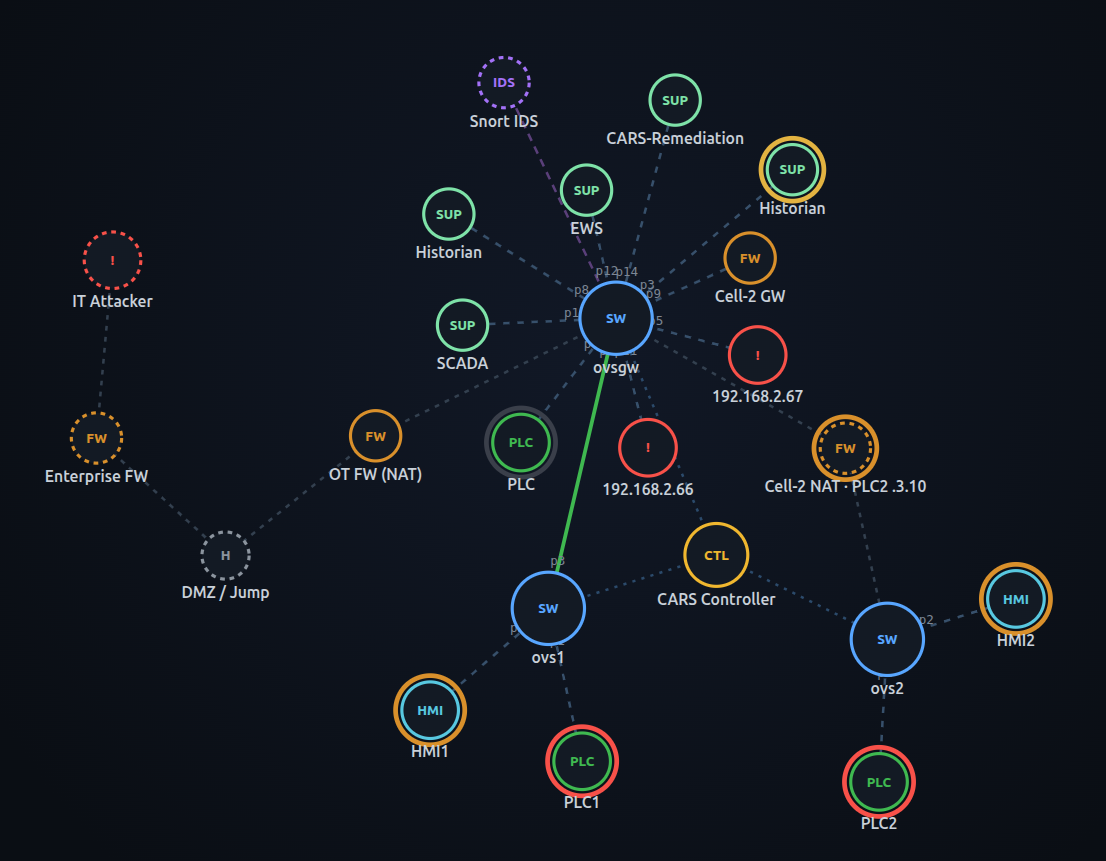
\includegraphics[width=0.9\textwidth]{dash_overview.png}
\caption{The CARS dashboard's discovered topology. Switches (\texttt{ovsgw}, \texttt{ovs1}, \texttt{ovs2}) in blue, the supervisory hosts (EWS, SCADA, the historians, CARS-Remediation) and PLCs discovered live with their roles and criticality rings, the CARS controller and Snort IDS, the modelled north side (Enterprise firewall, DMZ/jump, OT NAT) and the Cell-2 NAT path to PLC2. Unregistered hosts (the on-segment attacker seams \texttt{192.168.2.66} and \texttt{192.168.2.67}) are flagged. Everything shown is polled live from the controller, not drawn by hand.}
\label{fig:dashtopo}
\end{figure}

The centre of the view is the discovered network topology (Figure~\ref{fig:dashtopo}); the right-hand column carries the live decision feed, filterable by criticality tier, response, operation class and enforcement mode. Each row shows the source and its discovered role, the destination and its criticality tier, the operation class, the criticality-elevated tier and the selected response, colour-coded by severity. It is this feed that makes the engine's reasoning legible in real time: a supervisory read appears as an OPERATIONAL ALLOW, a remediation write as a RESTORE, and an out-of-role actuation as a FORBIDDEN ISOLATE.

Figure~\ref{fig:dashisolate} in Section~\ref{sec:evalcampaign} is a capture of this feed during the armed false-data-injection run: the compromised supervisory host \texttt{192.168.2.31 (scada)} issuing S7 CONTROL to the CRITICAL PLC1, each attempt classed FORBIDDEN and met with an ENFORCED ISOLATE. Placed beside the datapath rule of Figure~\ref{fig:p6armedflow} and the wire capture of Section~\ref{sec:evalcrosslayer}, it is the same attack seen at a third layer, the operator's, completing the cross-layer account: one event visible at once as a policy decision, an installed flow and a dropped packet.

\section{Gap remediation evidence}
\label{appx:gapevidence}

This appendix collects the fresh before-and-after evidence for the late-stage gap remediations of Chapter~\ref{chap:evaluation}, captured on 7 and 8 August 2026 on the armed testbed and returned to green after each run. The consolidated record with reproduction commands is the companion file \texttt{GAP\_REMEDIATION\_EVIDENCE.md}; the raw artefacts (controller-audit slices, the \texttt{cars.rules}/\texttt{cars.conf} diffs, the guardian log and the honeypot captures) are in \texttt{gap\_evidence/}.

\noindent\textbf{Gap A: DPI defeated by fragmentation, then hardened.} A Write-Var split across two TCP segments evaded the fixed-offset single-packet rule; after enabling stream reassembly and re-anchoring the rules to the S7 job header it is recovered and isolated at more than one split point, with the legitimate loop still permitted.
\begin{lstlisting}[style=carsdump,caption={Gap A: before (fragmented write evades) and after (caught), from the controller audit.},label={lst:ev_dpi}]
BEFORE (single-packet rules) - fragmented at byte 14, armed:
  192.168.2.31(scada) -> 192.168.2.10(plc) TCP => ALLOW (operational)   [no CONTROL recovered; 0xca=0; write reached PLC]
  (same write sent WHOLE):
  FORBIDDEN 192.168.2.31(scada) -> 192.168.2.10(plc) S7 CONTROL => ISOLATE source 192.168.2.31 75s
AFTER (stream5 reassembly + PDU-relative rules) - same fragmented attack:
  --split 14: FORBIDDEN 192.168.2.31 ... S7 CONTROL => ISOLATE source 192.168.2.31 75s ; flow 0xca nw_src=192.168.2.31
  --split  9: FORBIDDEN 192.168.2.31 ... S7 CONTROL => ISOLATE
  legit loop: OPERATIONAL 192.168.2.55(ews) -> 192.168.2.10 READ/CONTROL => ALLOW   [no new false positive]
\end{lstlisting}

The fix itself is shown as the unified diff of the deployed Snort configuration and rules against the pre-hardening backup: Listing~\ref{lst:ev_confdiff} adds the TCP stream-reassembly preprocessor on the ICS ports, and Listing~\ref{lst:ev_rulesdiff} re-anchors every S7 operation rule from a fixed packet offset to a PDU-relative match on the S7 job header.
\lstinputlisting[style=carsdump,caption={Gap A: \texttt{cars.conf} diff, stream reassembly added on ports 102 and 502.},label={lst:ev_confdiff}]{appendix_listings/gapA_cars_conf.diff}
\lstinputlisting[style=carsdump,caption={Gap A: \texttt{cars.rules} diff, S7 rules re-anchored PDU-relative (rev 1 to rev 2).},label={lst:ev_rulesdiff}]{appendix_listings/gapA_cars_rules.diff}

\noindent\textbf{Gap B: trusted-insider process guardian.} The high-rate overflow is cut by the volumetric overlay even from a trusted role; the read-only guardian then catches the low-rate denial and the high-side sensor spoof that the low-side remediation agent misses.
\begin{lstlisting}[style=carsdump,caption={Gap B: the flood backstop and the two guardian alarms.},label={lst:ev_guardian}]
FLOOD BACKSTOP (trusted .45 driven at high rate):
  192.168.2.45(remediation) -> 192.168.2.10 S7 CONTROL => [FLOOD 51 ops/s] BLOCK conduit 75s  [FDI cut after 77 writes; tank held ~mid-70s]
DEMO 1 - low-rate denial (one authorised HMI_Stop from .45):
  audit:    192.168.2.45(remediation) -> 192.168.2.10 S7 CONTROL => ALLOW (operational)   [network correctly permits]
  guardian: [GUARDIAN] ALARM STALL {level: 40.4, frozen_s: 12.0}                          [process halt caught]
DEMO 2 - spoof-to-high (reported level pinned at 90, real tank drains):
  remediation status: level=90.0, restores unchanged                                      [low-side agent silent = blind]
  guardian: [GUARDIAN] ALARM HIGH_LEVEL {level: 90.0, ceiling: 78.0}  +  ALARM RATE        [high-side caught]
\end{lstlisting}

The guardian writes each alarm to a read-only feed; the stall record from the fresh run is the raw line in Listing~\ref{lst:ev_guardianfeed}. This is a crafted scenario that demonstrates the mechanism rather than broad operational resilience: the flood, envelope and rate thresholds are tuned to this tank and its loop rate, and would need re-tuning for a different plant, loop cadence or operator profile.
\lstinputlisting[style=carsdump,caption={Gap B: the guardian alarm feed (\texttt{cars\_guardian.jsonl}), stall record from the fresh run.},label={lst:ev_guardianfeed}]{appendix_listings/gapB_guardian.jsonl}

\noindent\textbf{Gap C: flow-integrity poll window.} A rule injected and deleted inside the ten-second poll evades the auditor; a persistent one is caught within one poll. The single traces below were then repeated thirty times each to quantify the window: the persistent case was caught on every trial at a median of 8.5\,seconds, the two-second transient on only five of thirty (the runs whose life straddled a poll boundary). The per-trial values are in \texttt{gap\_evidence/flowint/persistent.csv} and \texttt{transient.csv}.
\begin{lstlisting}[style=carsdump,caption={Gap C: transient (mostly missed) versus persistent (always caught) flow-integrity status, with the thirty-trial totals.},label={lst:ev_poll}]
baseline:                     {"ok": 1, "extra": 0}
2 s transient inject+delete:  t+7s ok:1 | t+14s ok:1 | t+21s ok:1     [MISSED - never flipped]
persistent inject (left):     {"ok": 0, "extra": 1}                   [CAUGHT within one poll]
after cleanup:                {"ok": 1, "extra": 0}
30-trial totals:  persistent 30/30 caught, median 8.5 s | transient 5/30 caught, 25/30 evaded
\end{lstlisting}

The event-driven flow-monitor of Section~\ref{sec:threats} was then run against the identical thirty-trial transient test. It subscribes to the switch's Nicira flow-monitor (\texttt{ovs-ofctl monitor <br> watch:}) and, on any change to the policy tables that is not a cookie-\texttt{0xca} reactive rule, re-runs the deployed auditor's trusted check at once, so the sub-poll window closes without changing the verdict logic. Every one of the thirty two-second injections was caught, at a median of 0.27\,seconds, against five of thirty for the ten-second poll; the per-trial values are in \texttt{gap\_evidence/flowint/transient\_eventdriven.csv}.
\begin{lstlisting}[style=carsdump,caption={Gap C remedy: event-driven monitor on the same transient test.},label={lst:ev_poll_fix}]
10 s poll (baseline):     transient  5/30 caught, 25/30 evaded (median 8.5 s when caught)
event-driven monitor:     transient 30/30 caught, median 0.27 s   [sub-poll gap closed]
mechanism: NXST_FLOW_MONITOR watch -> immediate trusted re-check on any non-0xca policy-table change
\end{lstlisting}

\noindent\textbf{Gap 2: conduit block at a shared / NAT-collapsed identity.} An IT attacker source-NATed onto the gateway identity \texttt{192.168.2.1} was originally cut by a source isolation, which quarantines every host behind the NAT (Section~\ref{sec:evalanatomy}). The response selection was refined so a shared identity is cut at the conduit instead. Verified on the deployed engine: the same forbidden attempt from \texttt{192.168.2.1} now returns \texttt{BLOCK} and installs a conduit drop, while a true single host is still source-isolated.
\begin{lstlisting}[style=carsdump,caption={Gap 2: shared-identity conduit BLOCK versus single-host source ISOLATE, deployed engine.},label={lst:ev_natblock}]
gateway .1 (NAT-collapsed) -> CONTROL -> PLC1:  response=BLOCK
  flow: cookie=0xca priority=100,ip,nw_src=192.168.2.1,nw_dst=192.168.2.10 actions=drop   [conduit: only .1->PLC]
unknown .77 (true host)   -> CONTROL -> PLC1:  response=ISOLATE
  flow: cookie=0xca priority=110,ip,nw_src=192.168.2.77 actions=drop                       [source: whole host]
both land zero writes on the PLC; the gateway's non-PLC traffic is untouched by the conduit match.
\end{lstlisting}

\noindent\textbf{Gap D: DEFLECT diverts to the honeypot.} Forcing DEFLECT installs the redirect and the attacker's PLC-bound traffic arrives at the decoy while the real PLC sees nothing.
\begin{lstlisting}[style=carsdump,caption={Gap D: silent-drop baseline, the redirect, and the decoy receiving the diverted traffic.},label={lst:ev_deflect}]
silent-drop baseline:  atkns(.66) ping 192.168.2.10 -> 100% loss                       [dropped; attacker hangs]
force DEFLECT:         response=DEFLECT  action="DEFLECT conduit -> honeypot 192.168.3.99 (deception, self-healing)"
redirect flow:         priority=105 nw_src=192.168.2.66 nw_dst=192.168.2.10 -> set ip_dst=192.168.3.99, goto t2 (n_packets=3)
honeypot capture:      IP 192.168.2.66 > 192.168.3.99: ICMP echo request               [attacker DIVERTED to decoy]
                       ARP, who-has 192.168.2.66 tell 192.168.3.99                      [decoy engaging]
\end{lstlisting}

\noindent This is a proof of concept for the redirect path, not evidence of robustness. A determined adversary who notices the diversion, fingerprints the decoy or changes tactics is outside what this test exercises; sustaining a convincing interactive decoy is carried as future work in Section~\ref{sec:futurework}.

\noindent The plaintext control channel (G1), state-exhaustion resilience (G3) and the file-based detection bridge under heavy load (G4) are verified but framed as bounded limitations in Section~\ref{sec:threats} rather than tested, for the reasons given there.

\section{Process-transparency and availability runs}
\label{appx:availability}

This section holds the raw artefacts behind the process-transparency claim of Section~\ref{sec:evalprocessrisk} and the reconnection test of Section~\ref{sec:threats}, captured on the armed testbed on 7 August 2026 and returned to green after each run.

\noindent\textbf{Transparency: armed against disarmed under matched load.} The two states were interleaved in short blocks over two hours so that any drift in the hardware-in-the-loop simulation fell on both equally. The per-second tank level, phase label, online flag and restore count are in \texttt{availability/interleaved.csv} (7{,}060 samples); the online-only summary is below. The means and spreads coincide and neither state left the control band, so arming the defence has no measurable effect on the process. As Section~\ref{sec:evalprocessrisk} states, this is strong evidence for the testbed and its hardware-in-the-loop tank rather than a universal guarantee for all industrial processes.
\begin{lstlisting}[style=carsdump,caption={Transparency: online-only level statistics per phase, from \texttt{interleaved.csv}.},label={lst:ev_transparency}]
disarmed:  n=3528  mean=51.5%  sd=12.8  min=25.5  max=71.3   (band 20-78, no excursion)
armed:     n=3530  mean=50.7%  sd=13.2  min=25.6  max=71.3   (band 20-78, no excursion)
EWS/SCADA legitimate throughput unchanged across both phases.
\end{lstlisting}

\noindent\textbf{Block-and-maintain and self-heal, measured at the process.} An allowlisted supervisory host launched a false-data injection at the CRITICAL PLC under the armed defence. The write was classified FORBIDDEN and the source isolated after nine packets with the criticality-scaled seventy-five-second timeout; the tank stayed within band for the whole block, the legitimate conduits kept flowing, and the restoration agent was never called. The rule then expired and the source returned to service with no operator action, the install-to-withdrawal spanning seventy-six seconds.
\begin{lstlisting}[style=carsdump,caption={Block-and-maintain under attack, then self-heal, from the armed run.},label={lst:ev_selfheal}]
t+0.0s   FDI write from 192.168.2.31(scada) -> 192.168.2.10(plc, CRITICAL) => FORBIDDEN
t+~0s    ISOLATE source 192.168.2.31 (cookie 0xca, hard_timeout=75s, both switches)
block    tank level held within band; legit EWS/HMI conduits uninterrupted; restore agent NOT called
t+76s    rule expired (SEND_FLOW_REM); source restored, no operator action; table back to baseline
\end{lstlisting}

\noindent\textbf{Reconnection jitter, two planes.} Restarting the passive Snort sensor left the live conduit's inter-frame timing indistinguishable from baseline; forcing a controller reconnection by delete-and-re-add opened a roughly twenty-second window with multi-second forwarding stalls and dropped the synchronous S7 session. The per-second timeline (level, legitimate packets per second, controller-attached flag, event marks) is in \texttt{availability/jitter\_timeline.csv} with the accompanying \texttt{hil.pcap}. As Section~\ref{sec:threats} sets out, that window largely reflects the heavy re-add and pipeline re-sync rather than a faithful crash against the \texttt{fail\_mode=secure} switches, so it is reported as an upper bound and the clean crash-transparency figure is left as future work. This measurement should not be read as a crash-resilience proof or a production-availability guarantee: a fail-secure switch under a forced delete-and-re-add is not the same as a real controller crash, and the deployment implication is left deliberately cautious.
\begin{lstlisting}[style=carsdump,caption={Reconnection jitter: the two planes contrasted.},label={lst:ev_jitter}]
Snort restart (passive, out-of-band):  inter-frame mean 4.90 ms vs 4.91 ms baseline, worst gap 33 ms vs 42 ms  [TRANSPARENT]
Controller del/re-add (forced):         ~20 s window, worst forwarding gap 4.2 s, S7 session dropped, manual reconnect  [UPPER BOUND, not a faithful crash]
\end{lstlisting}

\section{Statistical visualisations of the evaluation}
\label{appx:stats}

The figures below plot the measured data behind the Critical Evaluation. Each is generated directly from a captured result file, named in its caption, with no smoothing or illustrative curves; log axes are used where a range spans orders of magnitude.

\begin{figure}[h]
\centering
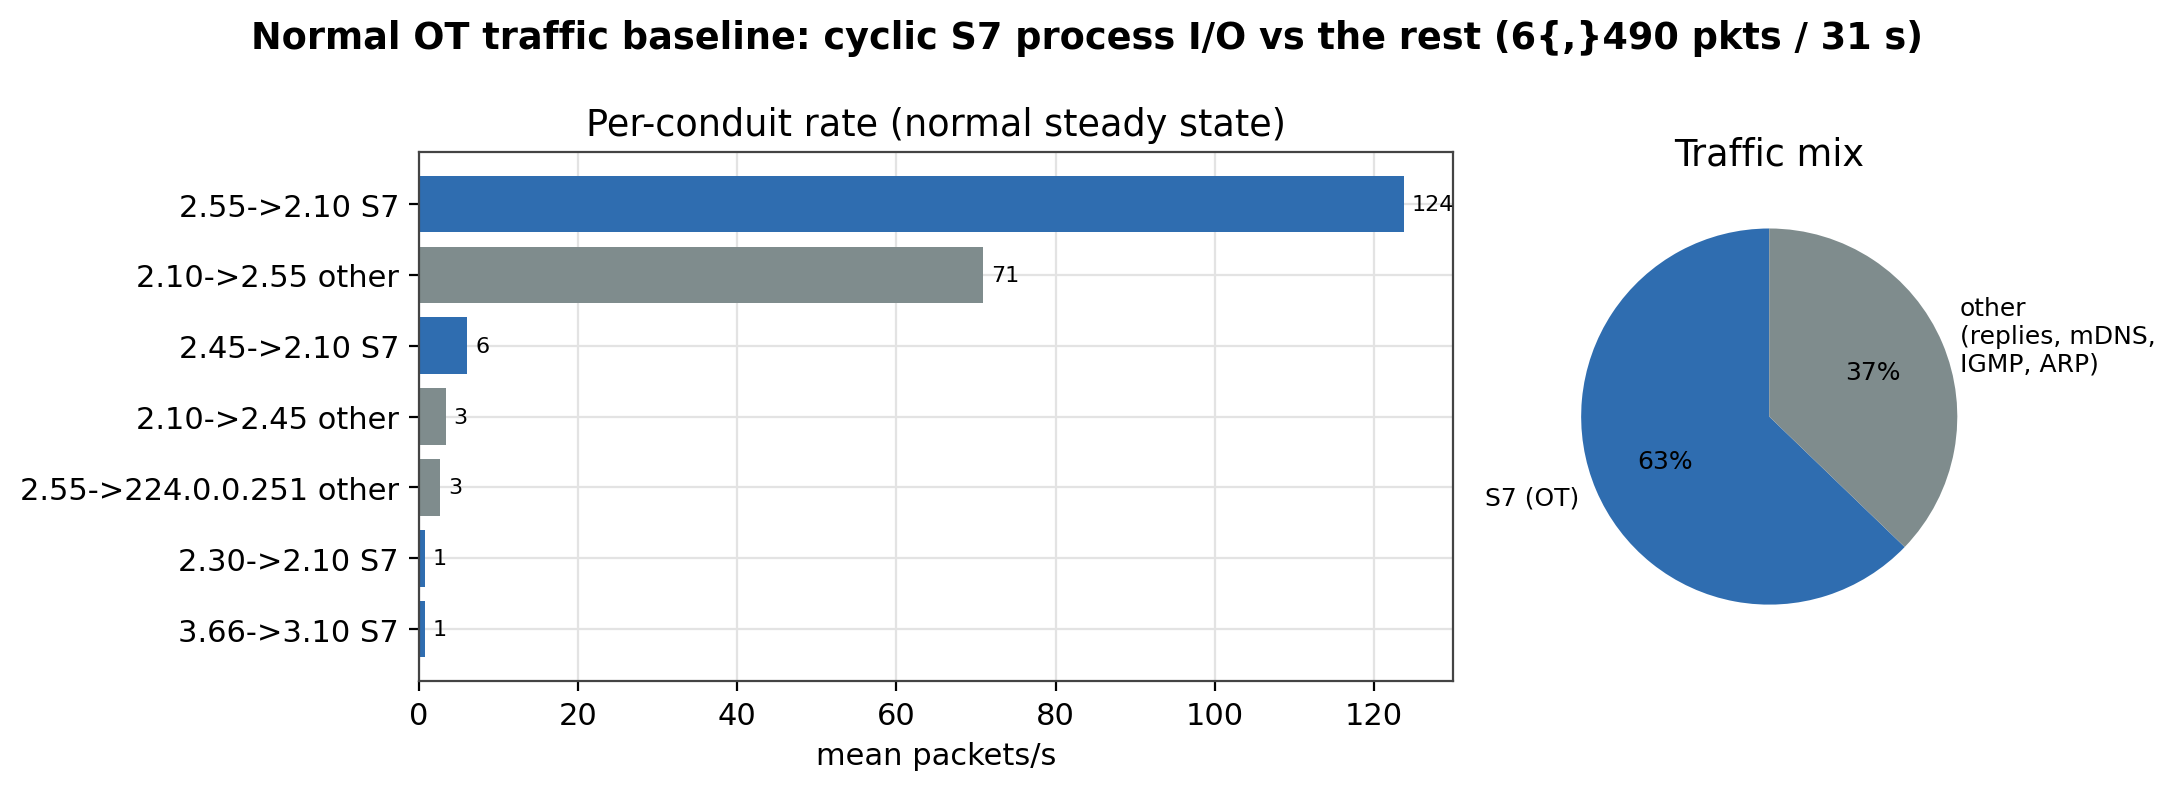
\includegraphics[width=0.95\textwidth]{stat_traffic_baseline.png}
\caption{Normal OT traffic baseline: per-conduit mean packets/s and the protocol mix, from a 31-second steady-state capture (6{,}490 packets, 9 conduits). The cyclic engineering-to-PLC S7 flow dominates; the remainder is PLC replies and background multicast. Source: \texttt{results/b1/baseline.pcap} via \href{\repourl/blob/main/07_Evaluation/overnight/b1_analyze.py}{\texttt{b1\_analyze.py}}.}
\label{fig:stattraffic}
\end{figure}

\begin{figure}[h]
\centering
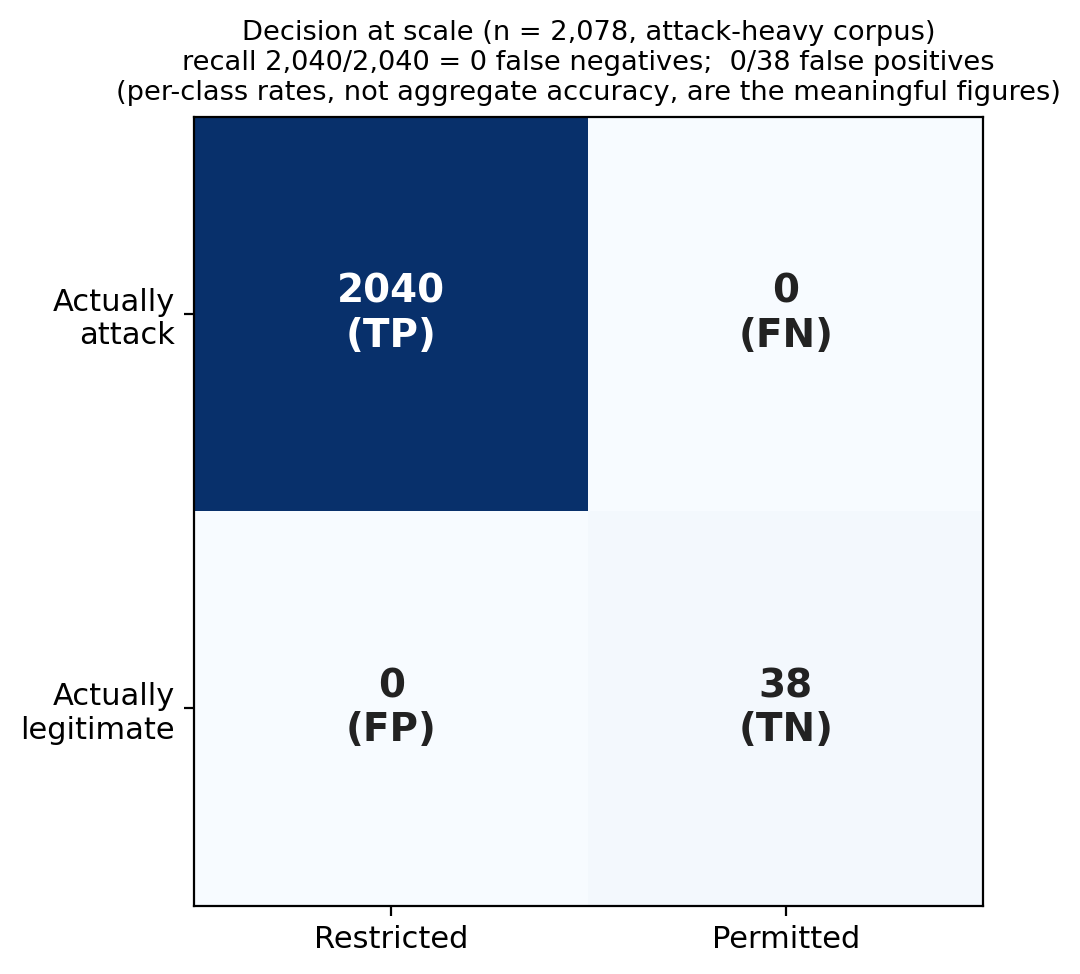
\includegraphics[width=0.62\textwidth]{stat_confusion.png}
\caption{Decision conformance at scale over the 2{,}078-case labelled corpus, which is attack-heavy by design (2{,}040 attacks against 38 legitimate or exempt cases). Every attack was restrained (no false negative) and every legitimate or exempt case permitted (no false positive). Because the decision is deterministic and the corpus is imbalanced, the two per-class error rates, both zero, are the meaningful figures rather than any aggregate. The attack side, where the label and the default-deny share the same registration test, is a coverage-and-robustness result; the zero false positive over the authorised cases is the trust result. Source: \texttt{results/vast/vast.csv}.}
\label{fig:statconfusion}
\end{figure}

\begin{figure}[h]
\centering
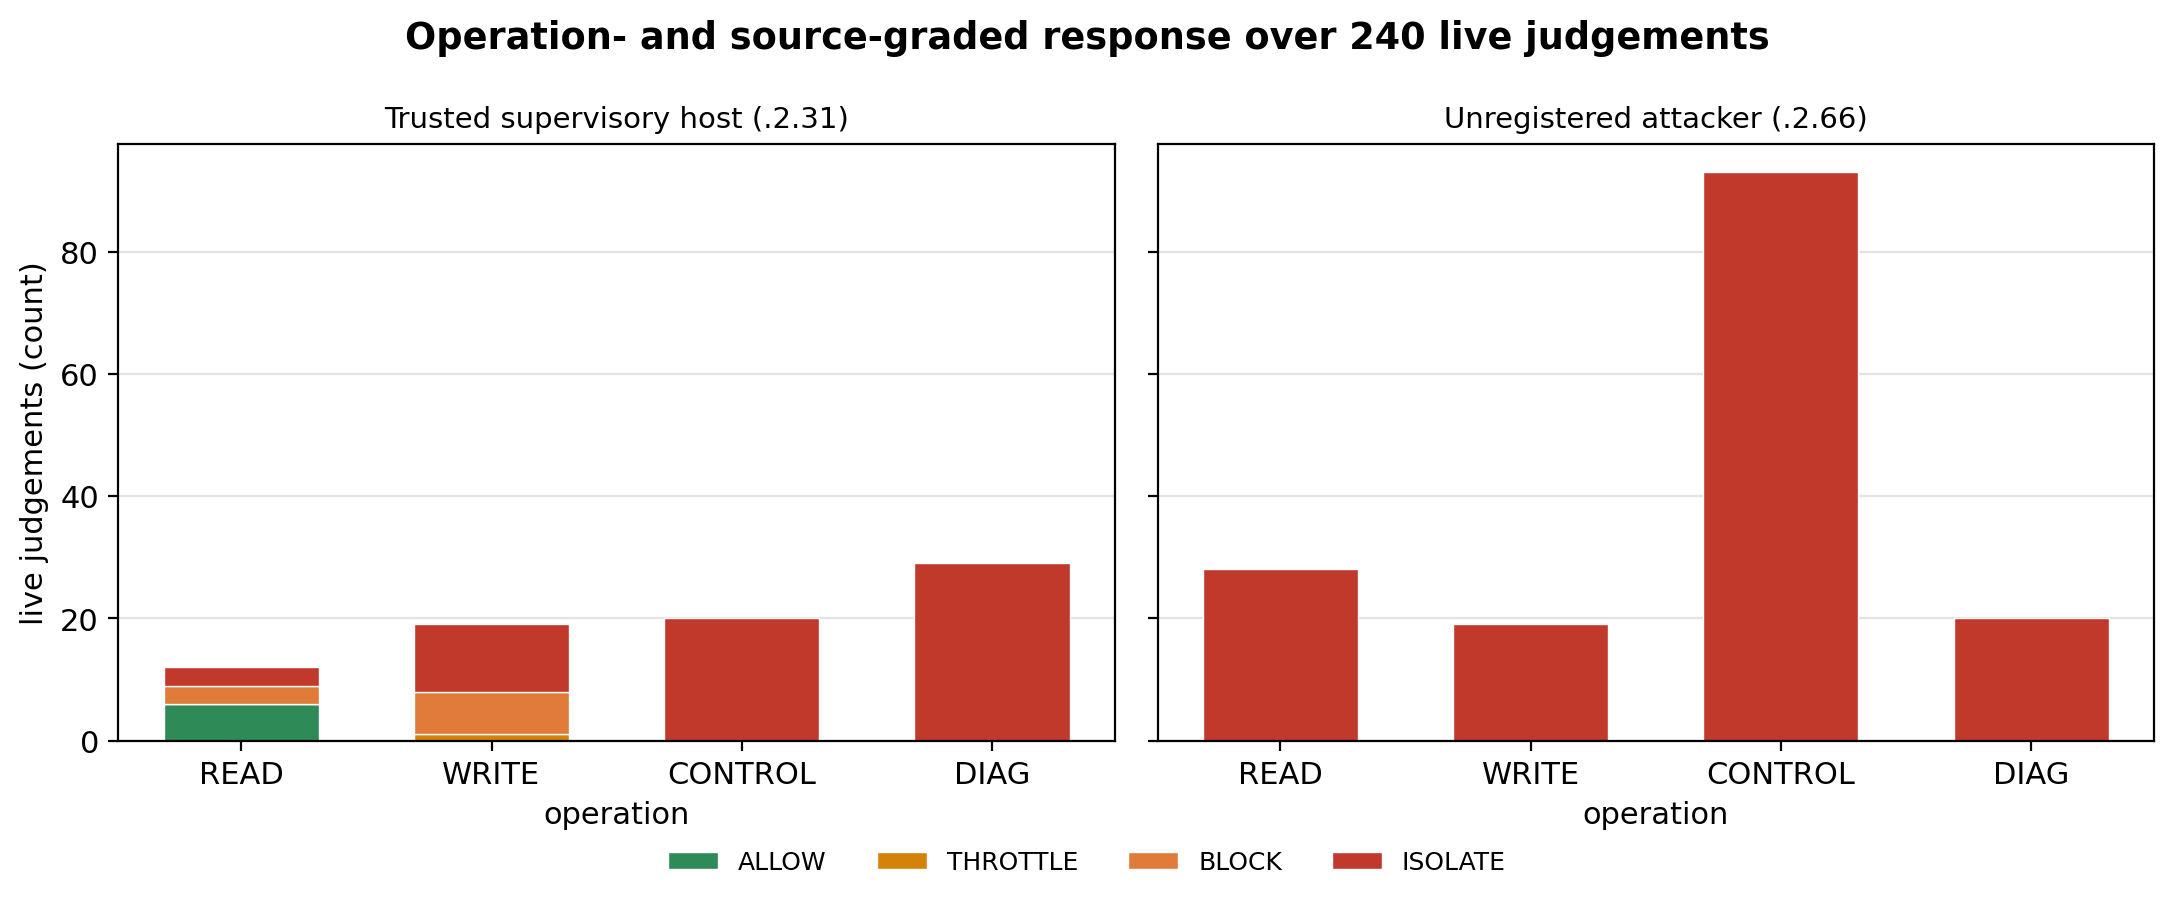
\includegraphics[width=0.98\textwidth]{stat_criticality_surface.png}
\caption{Operation- and source-graded response over 240 live judgements. The trusted host keeps its reads (with a small tail of persistence-escalated cuts as its offence count rises across the sequence) and is cut on the operations its role must not perform, whereas the unregistered attacker is cut on every operation. Source: \texttt{results/critbeh/judgements.csv}.}
\label{fig:statcrit}
\end{figure}

\begin{figure}[h]
\centering
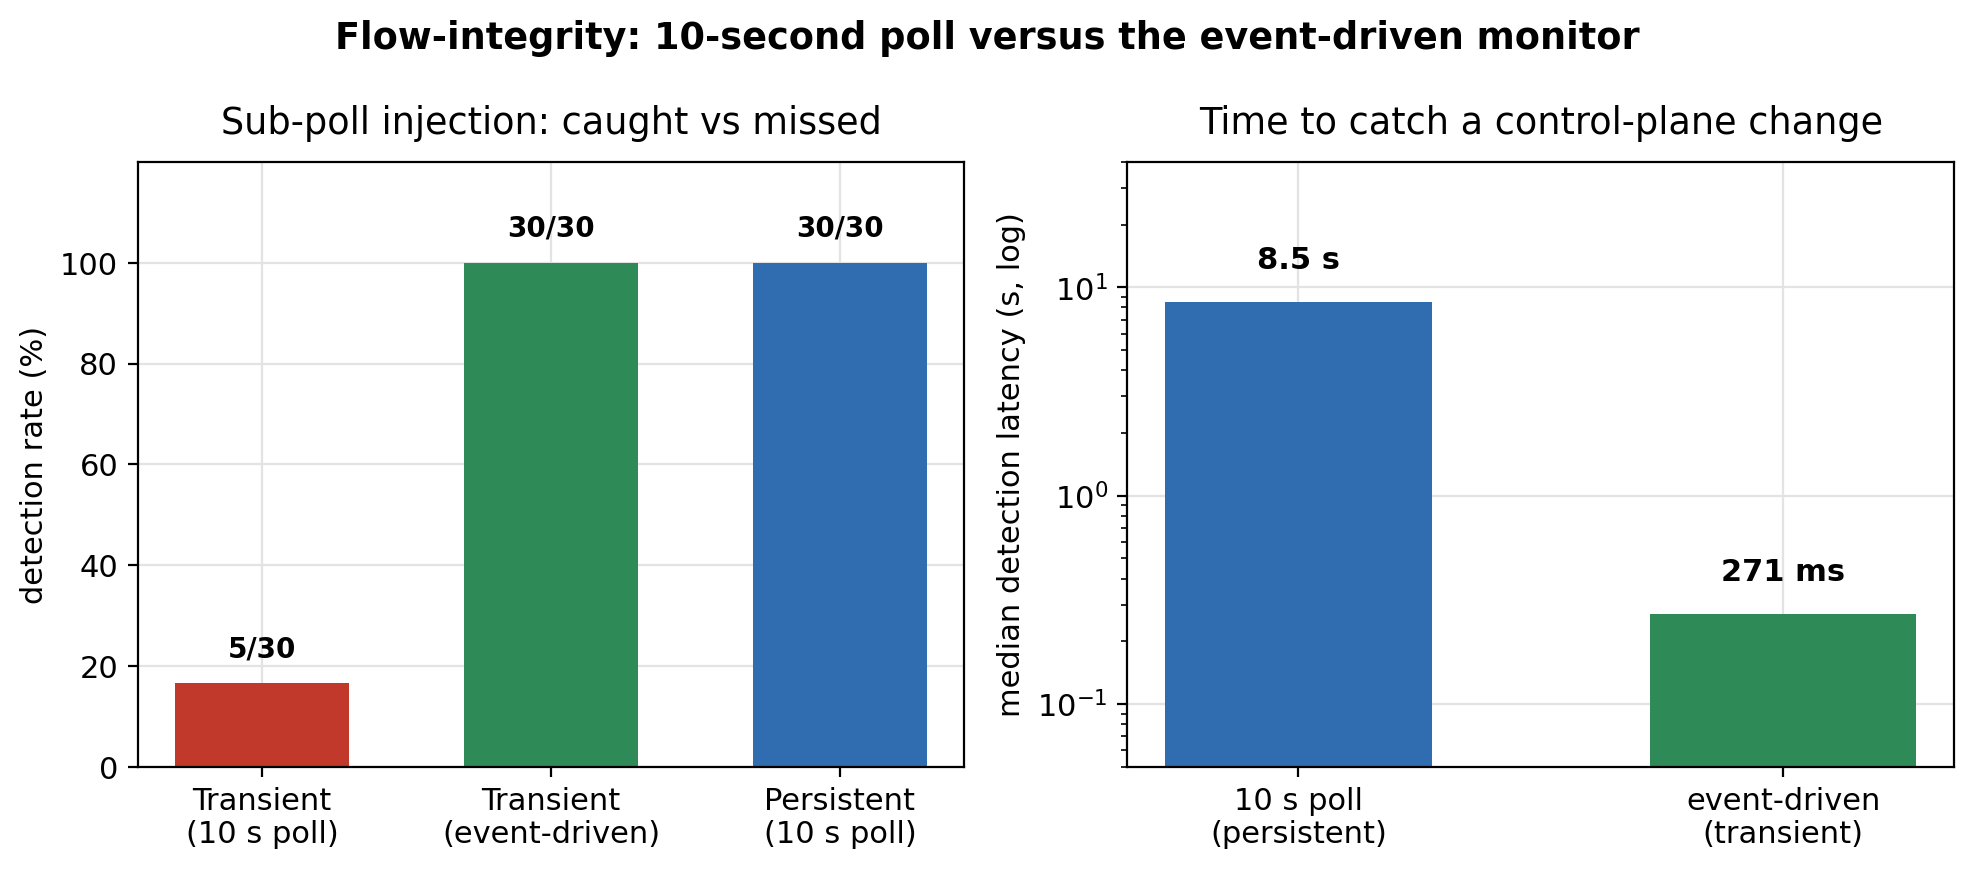
\includegraphics[width=0.95\textwidth]{stat_flowintegrity.png}
\caption{Flow-integrity, ten-second poll versus the event-driven monitor. Left: a two-second transient injection is missed by the poll on 25 of 30 trials but caught on all 30 by the event-driven monitor; a persistent injection is caught by both. Right: median detection latency, 8.5\,s for the poll against 0.27\,s for the monitor (log axis). Sources: \texttt{results/flowint/\{persistent,transient\}.csv}, \texttt{results/gap4\_flowmonitor/transient\_eventdriven.csv}.}
\label{fig:statflowint}
\end{figure}

\begin{figure}[h]
\centering
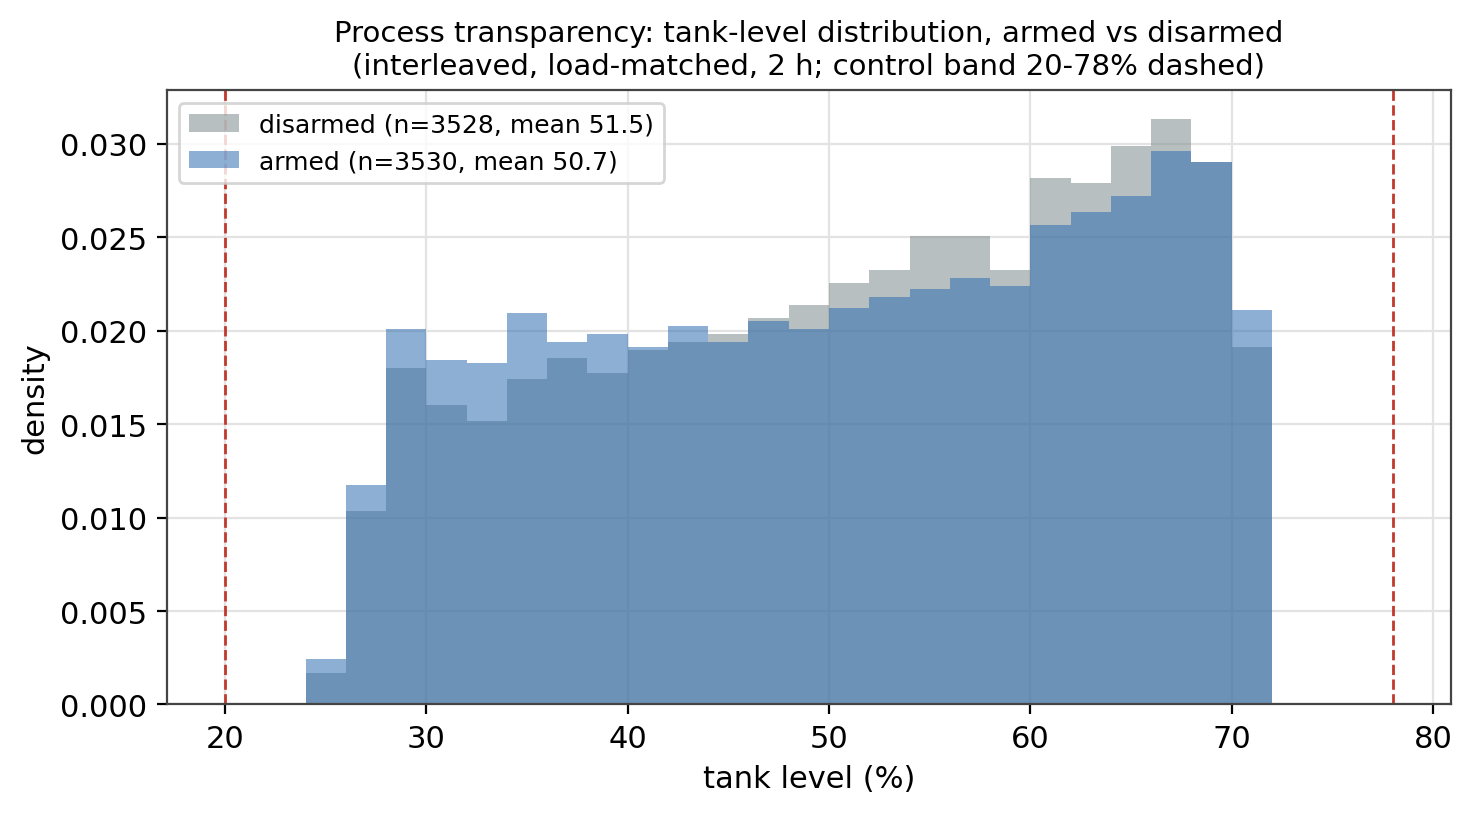
\includegraphics[width=0.8\textwidth]{stat_transparency.png}
\caption{Process transparency: the tank-level distribution armed against disarmed, over roughly seven thousand interleaved, load-matched per-second samples. The two distributions coincide (means 51.5 against 50.7\%) and neither leaves the control band, so arming the defence has no measurable effect on the process. Source: \texttt{results/e2/interleaved.csv}.}
\label{fig:stattransparency}
\end{figure}

\begin{figure}[h]
\centering
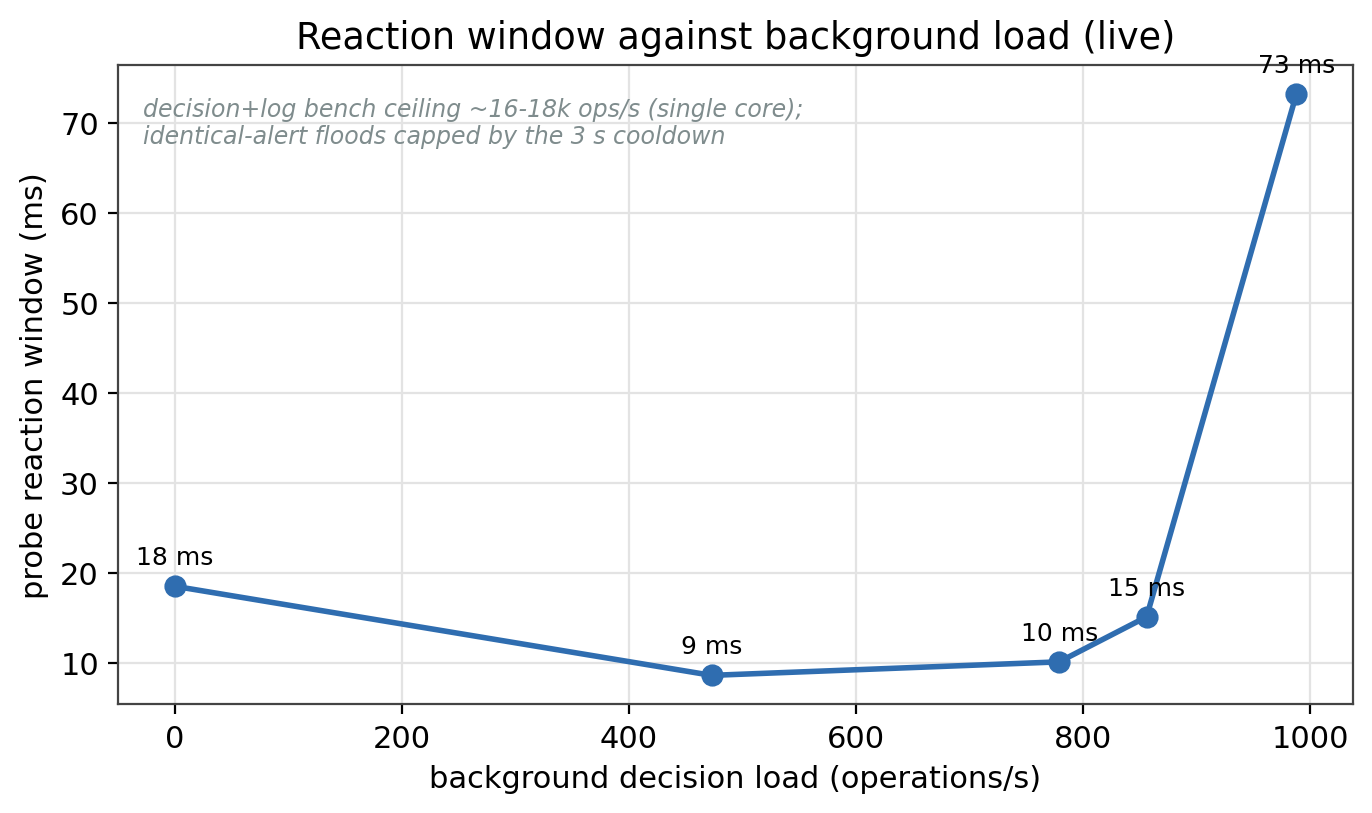
\includegraphics[width=0.78\textwidth]{stat_mttm_load.png}
\caption{Reaction window against background load, measured at the controller's decision-and-log stage: both the background and the probe are posted directly to \texttt{/cars/respond}, so this characterises the controller (\texttt{classify}, \texttt{select\_response} and the audit write), not the Snort-to-file-to-HTTP sensor bridge. The window holds in the tens of milliseconds to about a thousand operations a second and rises only as this single-threaded stage nears its sixteen-to-eighteen-thousand-a-second bench ceiling. The sensor bridge is a separate and lower ceiling, the acknowledged bottleneck carried to the future work (Section~\ref{sec:threats}), and is not what this curve measures. Source: \texttt{results/gap1\_live/curve.csv}.}
\label{fig:statload}
\end{figure}

\begin{figure}[h]
\centering
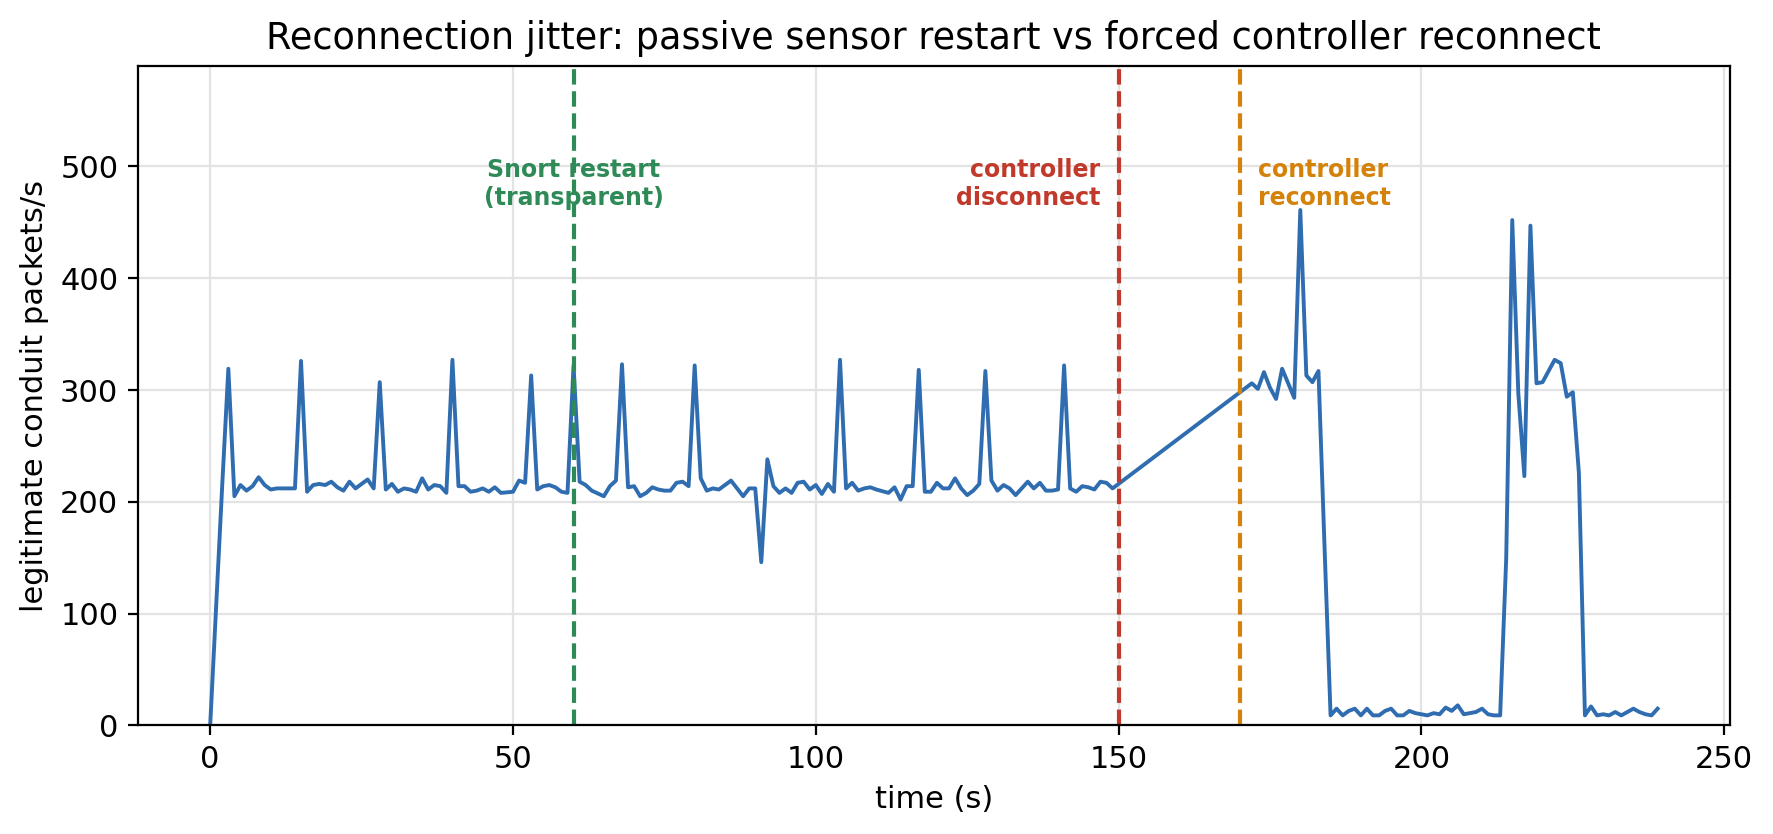
\includegraphics[width=0.92\textwidth]{stat_jitter.png}
\caption{Reconnection jitter on the legitimate conduit: restarting the passive Snort sensor is transparent (no dip), whereas a forced controller reconnection stalls forwarding. Source: \texttt{results/jitter/timeline.csv} (one spurious counter sample removed).}
\label{fig:statjitter}
\end{figure}

\subsection{Long-run and stress-test campaign}
\label{appx:longrun}

The figures below back the long-run and stress test of Section~\ref{sec:evallongrun}: four autonomous runs on the one testbed, 440 measured attacks, all enforced. They extend the earlier evidence in duration and repetition, not in network size. The four runs are repeated runs on the same testbed and machine state, not independent replicates; where a median is quoted it is pooled across the runs rather than averaged across per-run medians. Each plot is generated directly from the per-run \texttt{logs/*.csv} by \href{\repourl/blob/main/07_Evaluation/overnight/night/night_analyze.py}{\texttt{night\_analyze.py}}, with the row counts and any exclusions stated in the caption.

\begin{figure}[h]
\centering
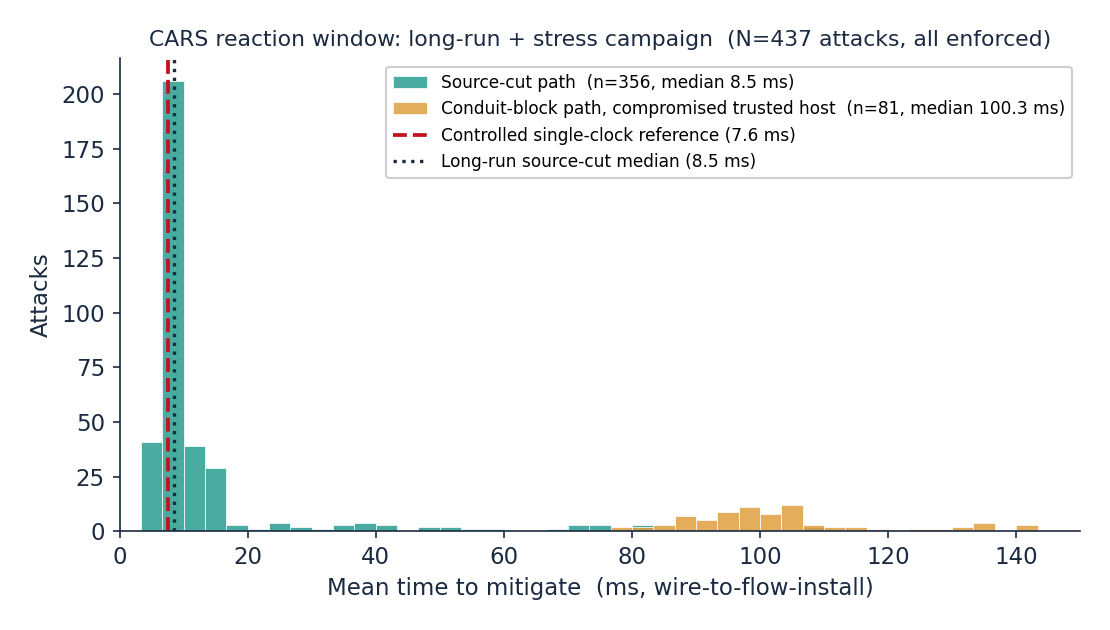
\includegraphics[width=0.95\textwidth]{stat_longrun_mttm.png}
\caption{Reaction window over the long-run and stress campaign. The source-cut path (356 attacks, median 8.5\,ms) sits close to the 7.6\,ms controlled single-clock reference of Section~\ref{sec:evallatency}; the false-data injections from the compromised trusted host form a separate mode near 100\,ms, the conduit-block path that installs after the first packets. 437 of the 440 measured attacks are shown: two under-load DDoS-probe samples, which belong to the load curve rather than the clean reaction window, and one physically impossible negative row from a stale-rule read, are excluded. Source: the four \texttt{night\_*/logs/mttm\_all.csv}.}
\label{fig:statlongmttm}
\end{figure}

\begin{figure}[h]
\centering
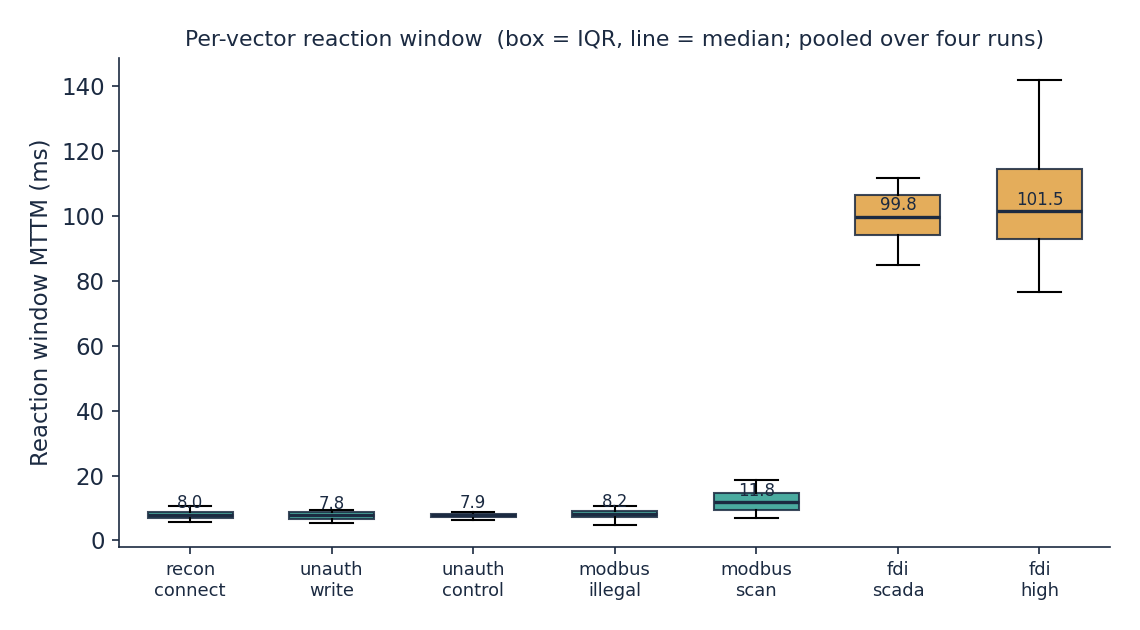
\includegraphics[width=0.95\textwidth]{stat_longrun_pervector.png}
\caption{Per-vector reaction window pooled over the four runs (box is the interquartile range, line the median). The source-cut vectors sit at roughly 7 to 12\,ms; the two false-data injection vectors from the compromised trusted host sit near 100\,ms because they draw a conduit block rather than an immediate source cut. Source: \texttt{night\_*/logs/mttm\_all.csv}.}
\label{fig:statlongpervec}
\end{figure}

\begin{figure}[h]
\centering
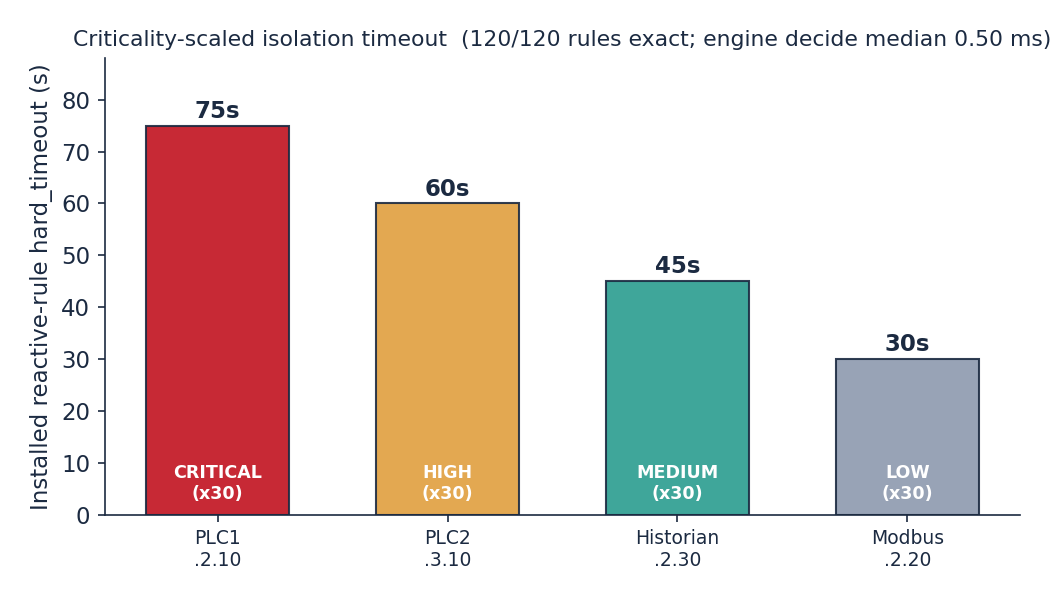
\includegraphics[width=0.9\textwidth]{stat_longrun_tierladder.png}
\caption{Criticality-scaled isolation timeout over 120 tier probes across the four runs. Every probe installed 75/60/45/30\,s for CRITICAL/HIGH/MEDIUM/LOW with no deviation, at a median engine decide-time of 0.50\,ms. Source: \texttt{night\_*/logs/tierladder.csv}.}
\label{fig:statlongtier}
\end{figure}

\begin{figure}[h]
\centering
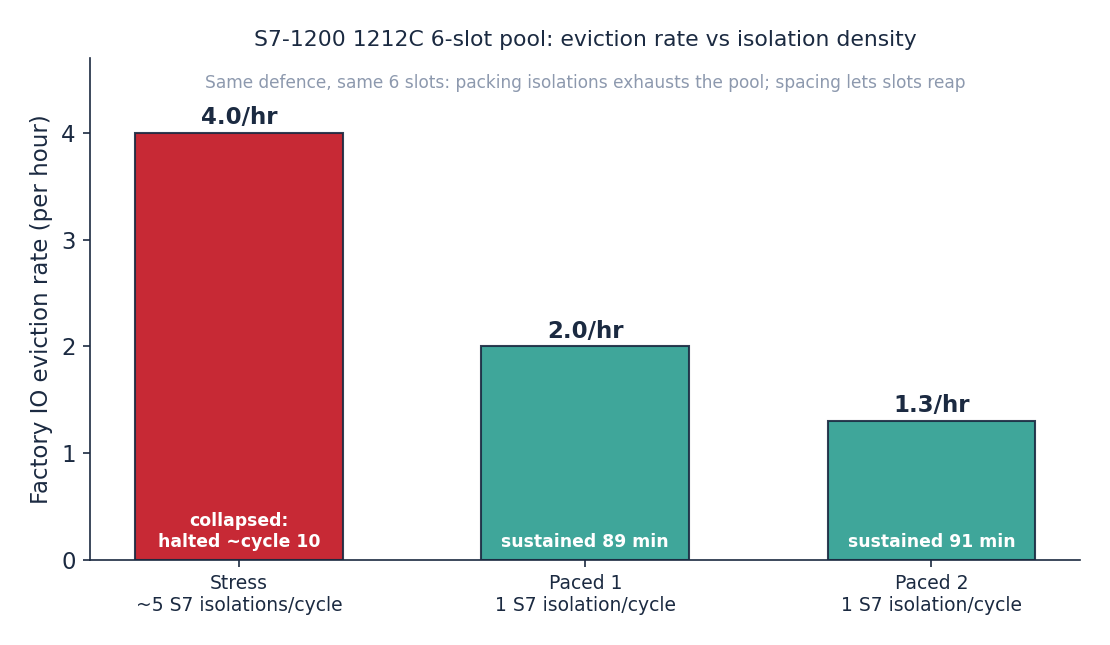
\includegraphics[width=0.95\textwidth]{stat_connpool_gradient.png}
\caption{The S7-1200 (1212C) connection-pool limit. The CPU exposes six dynamic connection resources; repeatedly isolating S7 sessions leaves half-open sessions that consume them. Packing about five isolations into each short cycle evicted the legitimate Factory IO client at 4.0 times an hour and the run could not be sustained; pacing to one isolation per cycle held the process for about ninety minutes at 1.3 to 2.0 evictions an hour. This is the empirical confirmation of the connection-pool caveat in Section~\ref{sec:threats}. Source: \texttt{night\_*/logs/\{freeze,monitor,mttm\_all\}.csv}.}
\label{fig:statconnpool}
\end{figure}

That the freeze is the endpoint's limit rather than a defect in the policy is confirmed on the switch: an isolate installs a single drop scoped to the attacker's source address alone, so it cannot match the legitimate conduit. Listing~\ref{lst:connscope} is a live capture taken on \texttt{ovs1} while an isolation was in force, showing the reactive rule matching only \texttt{nw\_src=192.168.2.77} while the \texttt{192.168.2.55} to \texttt{192.168.2.10} conduit remained a committed allow with its counter advancing.

\lstinputlisting[style=carsdump,caption={The isolate is source-scoped: the reactive drop matches the attacker alone, and the legitimate Factory IO conduit is untouched during the isolation (captured live on \texttt{ovs1}).},label={lst:connscope}]{appendix_listings/conn_scope.txt}

\begin{figure}[h]
\centering
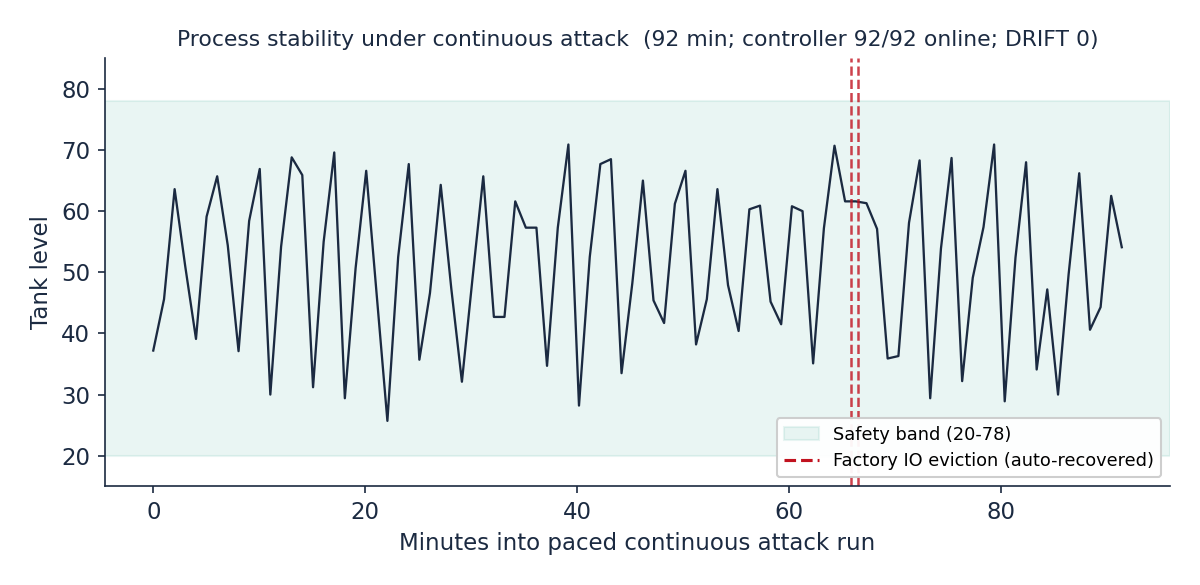
\includegraphics[width=0.98\textwidth]{stat_longrun_stability.png}
\caption{Process stability under continuous attack: the tank level across the ninety-two-minute paced run, held within the 20 to 78 control band throughout. The controller and its remediation agent reported the process online in all ninety-two one-minute snapshots (this is the agent's PLC link sampled once a minute, which does not capture sub-minute client outages) and the flow auditor reported no drift. The two dashed marks are the brief Factory IO client evictions that the liveness guard caught and recovered. Source: \texttt{night\_paw2\_0153/logs/\{monitor,freeze\}.csv}.}
\label{fig:statlongstab}
\end{figure}


\end{document}
